\documentclass{base}

\begin{document}

\cover
\newpage
\tableofcontents

\newpage


	\begin{center}
	\zihao{-3}
	\textbf{摘要}
\end{center}


本次我开发了一个以《星际迷航》为主题的星舰管理系统,为爱好者提供一个全面的星舰信息管理和查询平台。系统采用当前流行的技术栈,包括 Spring Boot 作为后端服务框架,Vue.js 作为前端界面框架,以及 MySQL 作为数据库支撑。通过该系统,用户能够实现对星舰及其武器的增删改查操作,并进行用户信息的个性化管理。

在项目开发过程中,我首先进行了详尽的需求分析,确保系统设计能够满足《星际迷航》爱好者的特定需求。我采用了文献综述法和问卷调查法,深入了解用户期望和《星际迷航》背景知识,为系统设计提供了坚实的理论和实践基础。

系统设计遵循模块化原则,明确划分了用户登录与注册、星舰管理、武器管理和用户信息管理等模块。开发过程中,前端与后端的分离确保了项目的灵活性和可维护性。通过使用 JWT 进行身份验证,系统提高了安全性。数据库设计上,我们采用了结构化和模块化的方法,并通过索引优化了查询效率。

在系统测试阶段,我使用了 Postman工具对后端 API 进行测试,同时利用浏览器控制台对前端进行调试和测试,确保了系统的稳定性和可靠性。
\\

\noindent\textbf{关键词:}星舰管理系统,Spring Boot,Vue.js,MySQL,用户管理,模块化设计,系统测试

\newpage


\begin{center}
	\zihao{-3}
	\textbf{Abstract}
\end{center}
\qquad This time I developed a starship management system with the theme of Star Trek to provide fans with a comprehensive starship information management and query platform. The system uses the current popular technology stack, including Spring Boot as the backend service framework, Vue.js as the front-end interface framework, and MySQL as the database support. Through this system, users can add, delete, modify and query starships and their weapons, and perform personalized management of user information.

During the project development process, I first conducted a detailed demand analysis to ensure that the system design can meet the specific needs of "Star Trek" fans. I used the literature review method and questionnaire survey method to deeply understand user expectations and Star Trek background knowledge, providing a solid theoretical and practical foundation for system design.

The system design follows the principle of modularization, and clearly divides modules such as user login and registration, starship management, weapon management, and user information management. During the development process, the separation of the front end and the back end ensures the flexibility and maintainability of the project. By using JWT for authentication, the system improves security. In database design, we adopted a structured and modular approach and optimized query efficiency through indexing.

During the system testing phase, I used the Postman tool to test the backend API and used the browser console to debug and test the front end to ensure the stability and reliability of the system.
\\

\noindent\textbf{Keywords:} Starship management system, Spring Boot, Vue.js, MySQL, user management, modular design, system testing

\newpage

\section{绪论}

本次小学期要求制作的网站与数据库相结合的管理系统,基本要求是:

\begin{enumerate}
	\item 前端使用 Vue.js;后端使用 Spring Boot。
	\item 建立其的前后端能够正常通信,并实现用户登录和数据库的增删改查。
\end{enumerate}

为了保证个人选题新颖,又能满足所要求的技术栈,我选择了制作以经典电影《星际迷航》为主题的\textbf{星舰管理系统}。
\subsection{研究背景与研究意义}
《星际迷航》(\textit{Star Trek})是美国一部极具影响力的科幻电视系列剧,由吉恩·罗登贝瑞(Gene Roddenberry)创作。自 1966 年首次播出以来,这个系列已发展成为一个庞大的跨媒体特许经营,包括电视剧、电影、小说、漫画和电子游戏等。

影视中的星舰庞杂、类别繁琐,为该影视的爱好者实现一个星舰管理系统,\textbf{不仅能够建立起一个类星际迷航的维基百科式站点,也能锻炼学生的开发能力,让学生在兴趣中开发,从而不断激发其潜能。}
\subsection{设计内容}
本项目以星舰舰长的视角,设计了用户登录模块、星舰管理模块、武器管理模块、用户信息管理模块。各模块之间均有联系。
\subsection{课题研究方法}

为了实现星舰管理系统的开发,本次研究采用了文献综述法,通过查阅大量关于《星际迷航》的影视资料、书籍和相关论文,深入了解《星际迷航》的背景、星舰类型和特点。结合管理系统开发的相关技术文献,分析现有管理系统的设计模式和实现方法,为本课题提供理论支持。

通过问卷调查和访谈的形式,了解《星际迷航》爱好者对星舰管理系统的需求,明确系统的功能要求和用户体验需求。根据调查结果,确定系统的功能模块和设计框架。

采用SpringBoot和Vue技术栈进行系统的设计与开发。系统设计阶段包括模块划分、数据库设计和界面设计;开发阶段包括后端服务的实现、前端界面的开发及前后端的集成。

在系统开发完成后,通过单元测试、集成测试和用户测试等方式对系统进行全面测试,发现并修复系统中的缺陷。根据测试结果和用户反馈,对系统进行优化和迭代改进。

\subsubsection{技术路线与工具选择}


前端技术使用Vue.js,用于构建用户界面。Vue.js 是一款渐进式JavaScript框架,具有响应式的数据绑定和组件化开发的特点,非常适合构建复杂的单页面应用(SPA)。Vue Router用于管理前端路由,实现页面的导航和切换。Axios用于发送异步请求,与后端API进行数据交互。

\begin{figure}[H]
	\centering
	
\includegraphics[width=0.7\linewidth]{images/vue-logo.png}
	\caption{Vue Logo}
	\label{fig:}
\end{figure}

后端技术使用Spring Boot,用于构建后端服务。Spring Boot 提供了开箱即用的配置和内嵌的服务器,使得开发、测试和部署变得更加简便。JPA (Java Persistence API):用于数据持久化操作,简化与数据库的交互。

\begin{figure}[H]
	\centering
	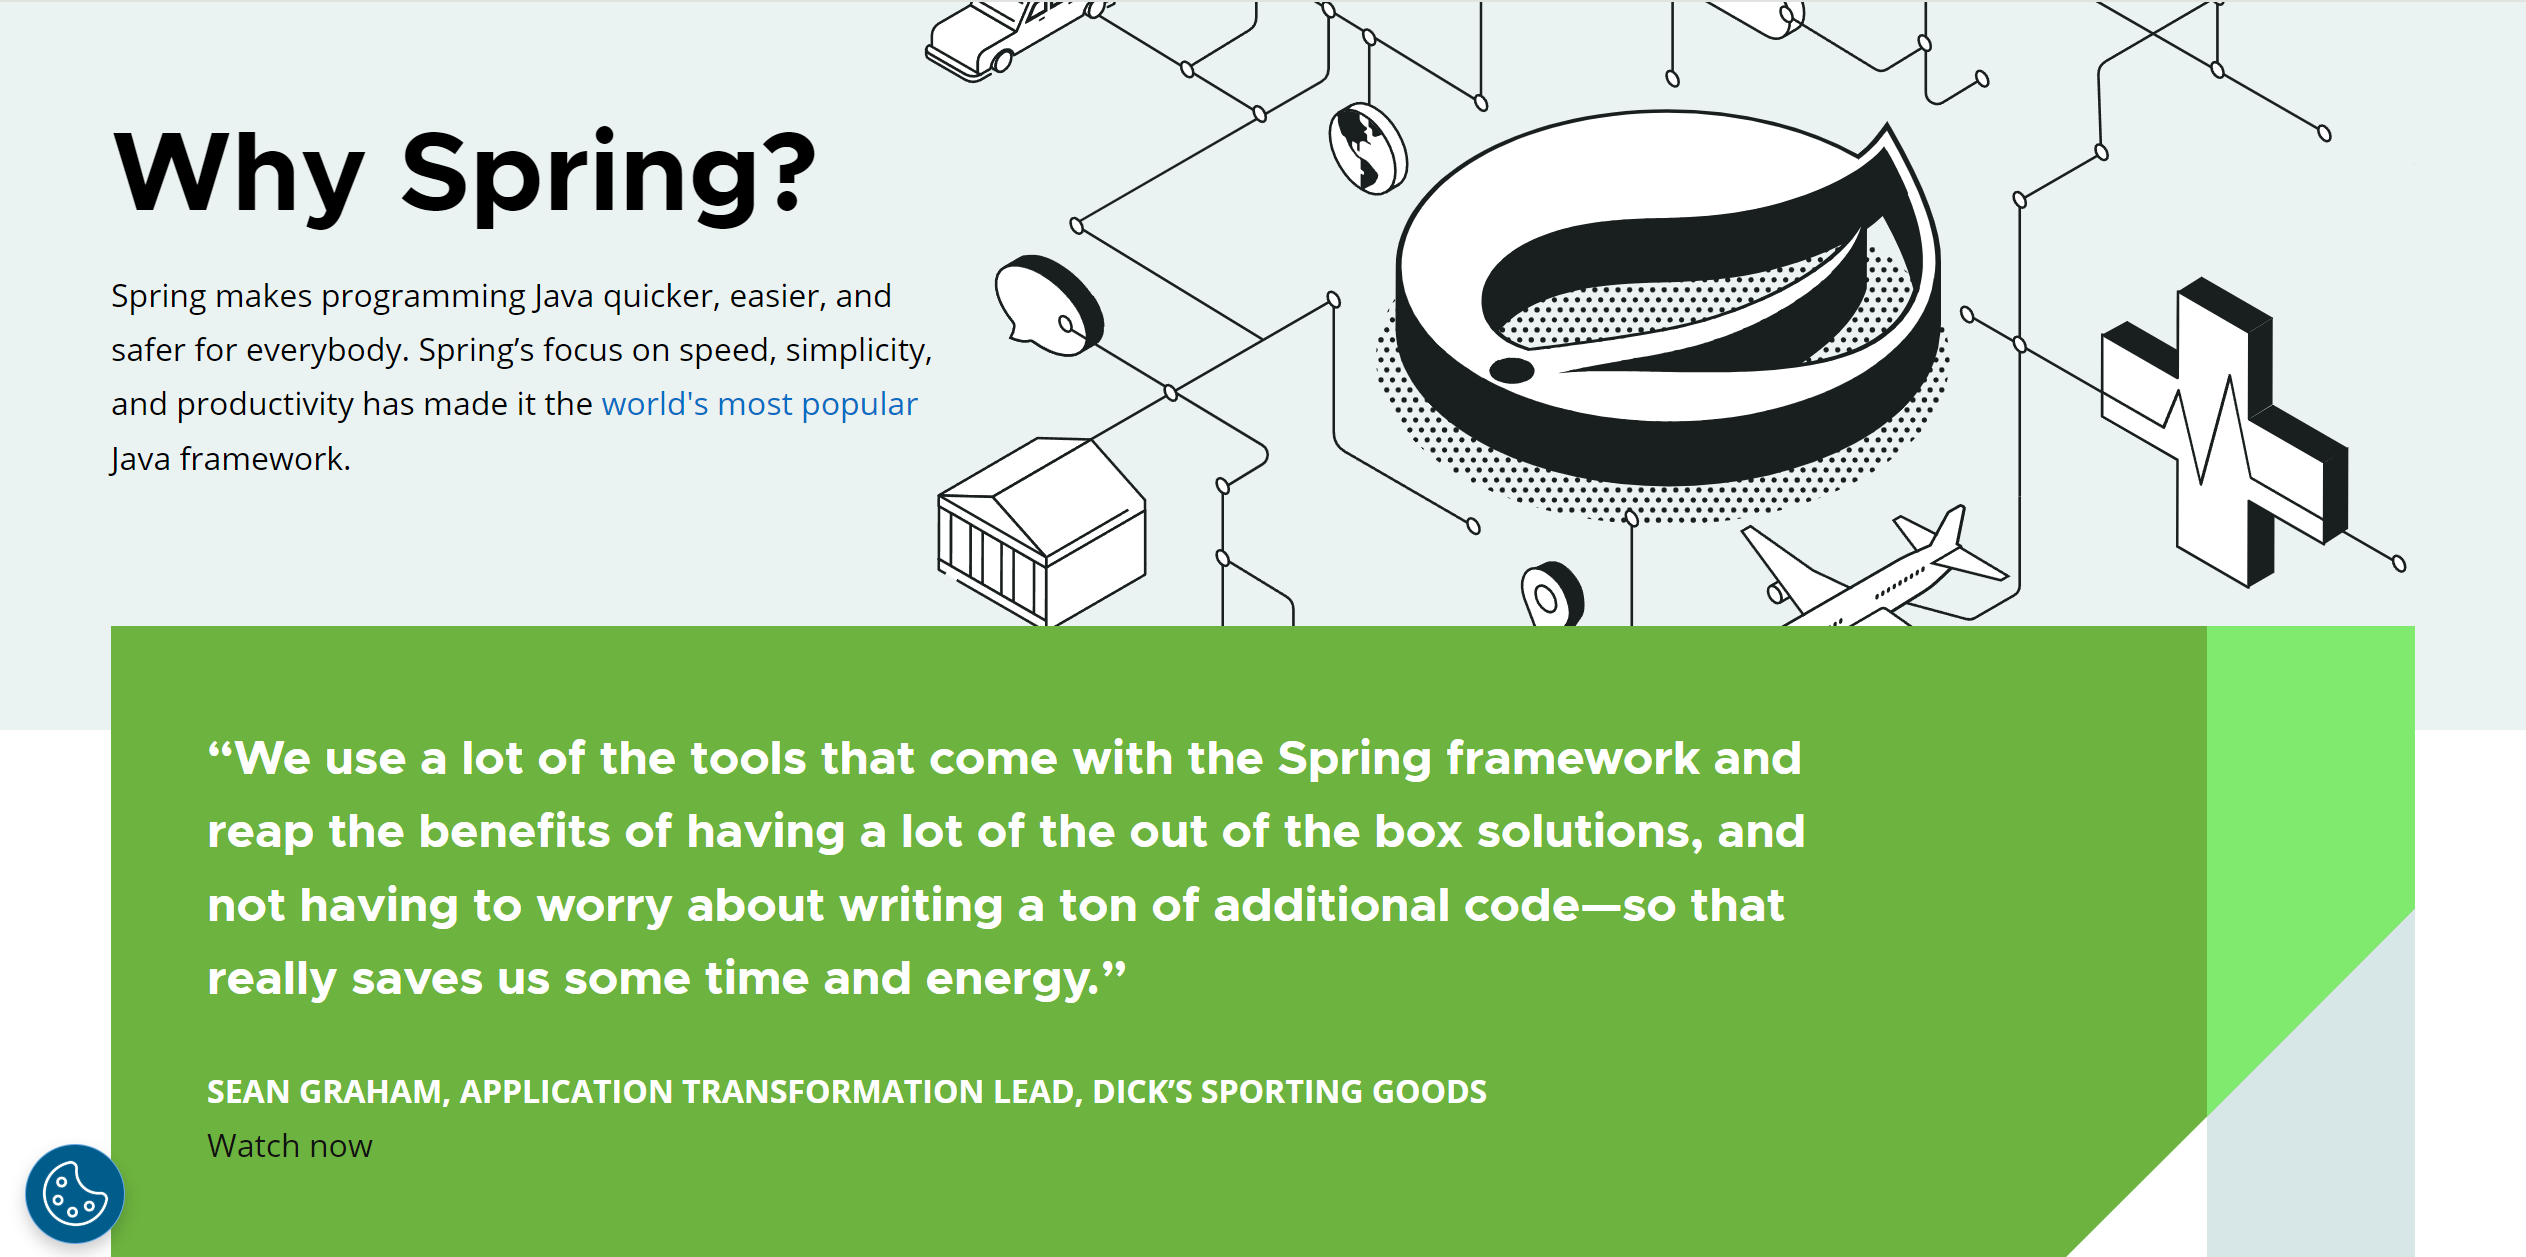
\includegraphics[width=0.7\linewidth]{images/spring-web.png}
	\caption{Spring Boot 网站首页}
	\label{fig:}
\end{figure}

数据库使用MySQL,作为关系型数据库,用于存储用户信息、星舰数据和武器数据。MySQL 具有高性能、稳定性好、使用方便等特点。

开发工具使用IDEA,用于前后端代码的开发和调试,支持Spring Boot项目的快速创建和配置。

测试时,Postman用于测试后端API,验证接口的正确性和性能。Postman是一款用于API开发、测试和调试的工具。它提供了一个直观的界面,用户可以轻松地发送HTTP请求、查看响应、组织API文档和测试API功能。Postman支持多种协议,如HTTP、HTTPS、WebSocket等,是开发者在进行API开发和测试时的重要工具。

\begin{figure}[H]
	\centering
	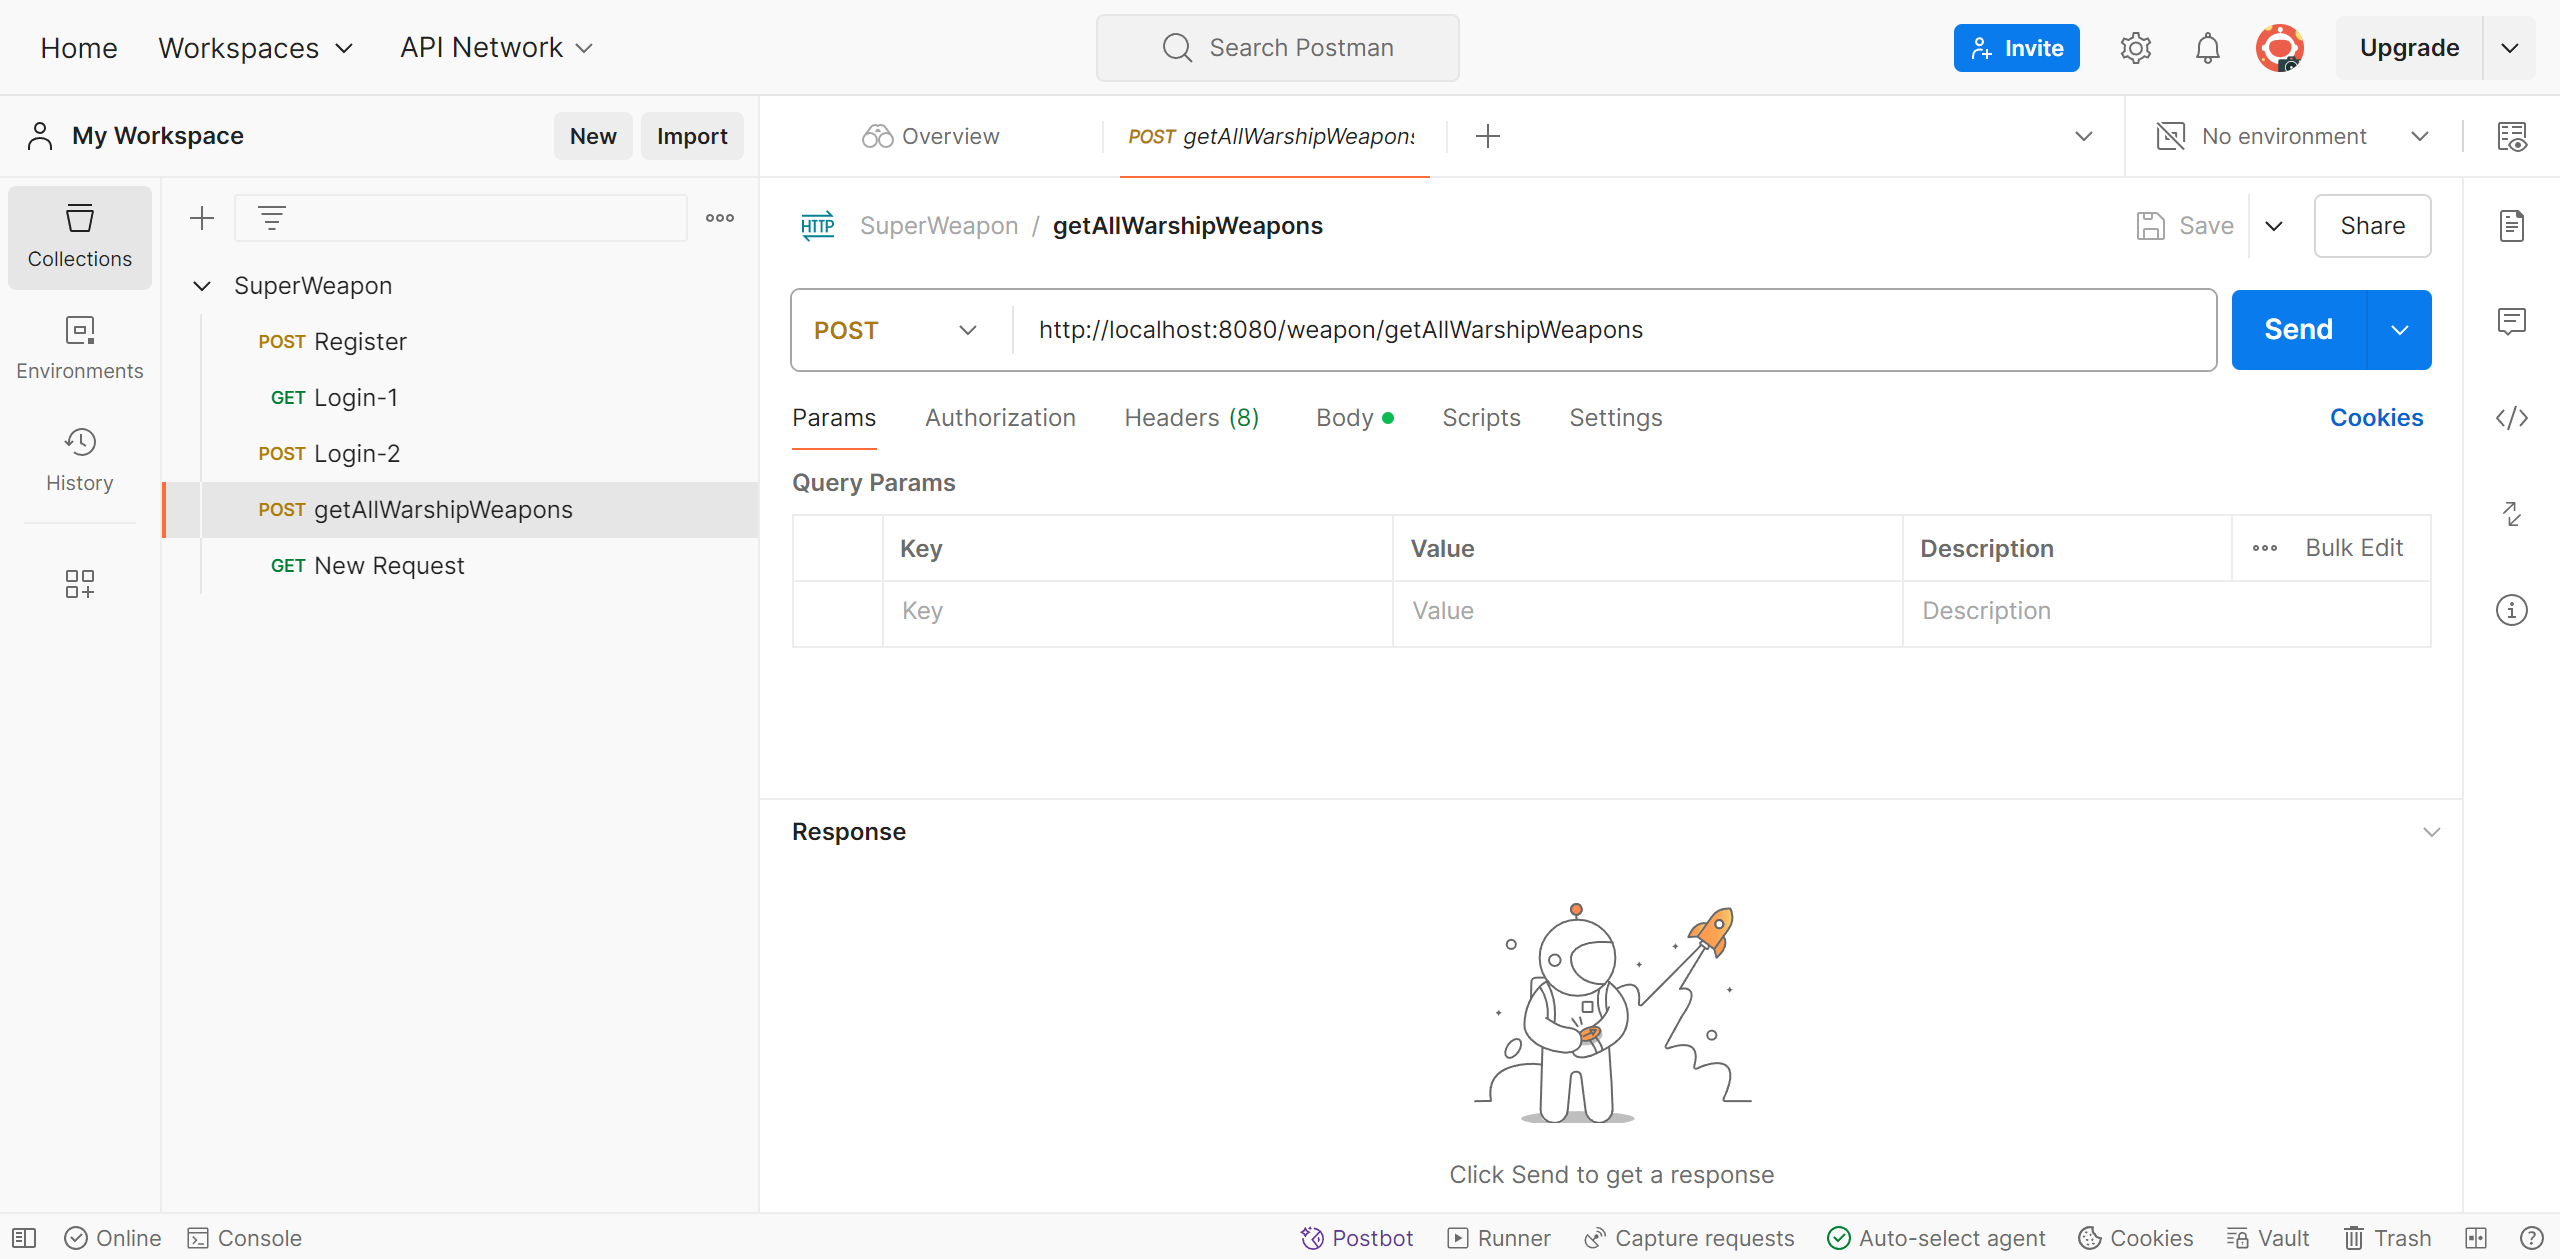
\includegraphics[width=0.7\linewidth]{images/postman.png}
	\caption{后端开发时,正在使用 Postman 进行测试}
	\label{fig:}
\end{figure}

版本管理则使用Git用于版本控制,方便代码的管理。

\subsubsection{开发环境与测试环境搭建}

本次开发需要安装的开发工具有 IDEA ,可通过访问 \url{https://www.jetbrains.com/idea/} 下载。

剩下的环境我们使用 Chocolatey 进行安装,它是一个Windows上的软件包管理器,可以通过命令行轻松安装、更新和管理软件包。

以管理员身份打开 PowerShell ,然后执行:
\begin{verbatim}
	Set-ExecutionPolicy Bypass -Scope Process -Force;
	
	[System.Net.ServicePointManager]::SecurityProtocol = 
	[System.Net.ServicePointManager]::SecurityProtocol -bor 3072; 
	
	iex ((New-Object System.Net.WebClient)
	.DownloadString('https://community.chocolatey.org/install.ps1'))
\end{verbatim}

随后的安装就很简单了,下面直接安装 node.js、mysql、maven、java JDK:
\begin{verbatim}
	choco install nodejs mysql maven jdk17
\end{verbatim}

\section{系统分析}

\subsection{系统可行性分析}

本章节主要评估星舰管理系统在技术、经济和操作方面的可行性。

\subsubsection{技术可行性}

系统采用 SpringBoot 和 Vue 技术栈,这两者都是当前流行且成熟的技术。SpringBoot 作为后端框架,具有快速开发、配置简单、社区支持丰富等优点,能够高效地实现复杂的业务逻辑和数据管理。Vue 作为前端框架,具有轻量、高效、易于学习和使用的特点,能够实现响应式和动态的用户界面。

数据库采用 MySQL,MySQL 是一个开源的关系型数据库管理系统,具有高性能、高可靠性和易于使用的特点,适合用于本项目的数据存储和管理。

\subsubsection{经济可行性}
系统开发所需的技术和工具(如 SpringBoot、Vue、MySQL 等)都是开源且免费的,这大大降低了开发成本。项目的开发团队主要由学生组成,不需要额外的人工成本。系统的部署可以选择免费的云服务器,进一步降低运行成本。

\subsubsection{操作可行性}
系统的用户主要为《星际迷航》的爱好者和开发团队成员。用户界面设计友好、易于操作,通过简单的注册和登录即可使用系统的各项功能。开发团队通过学习和实践,能够熟练掌握所需的技术和工具,确保项目的顺利进行。

\subsection{需求分析}

明确系统的功能需求和用户需求,为系统设计和开发提供依据。

\subsubsection{功能需求}
用户登录与注册,提供用户注册和登录功能,确保系统的安全性和个性化服务。
星舰管理,实现对星舰信息的增删查改,包括星舰名称、型号、所属舰队等信息。
武器管理,实现对星舰武器的增删查改,包括武器名称、类型、威力等信息。
用户信息管理,实现对用户信息的管理,包括用户名、邮箱、兴趣爱好等。
\subsubsection{用户需求}
便捷的操作界面,用户界面设计应简洁、美观,操作流程应简便,减少用户学习成本。
详细的星舰信息,提供详尽的星舰信息,包括历史背景、技术参数、服役情况等。
个性化服务,根据用户兴趣推荐相关的星舰和武器信息,提高用户体验。

\subsection{功能性要求}

功能性要求是对系统功能的详细描述,明确每个功能模块的具体实现。

\subsubsection{用户登录与注册模块}
\textbf{用户注册} 用户提供用户名、密码、邮箱等信息进行注册,注册信息保存到数据库。

\textbf{用户登录} 用户输入用户名和密码进行登录,系统验证用户信息,成功登录后进入系统主界面。

\subsubsection{星舰管理模块}

\textbf{新增星舰} 可以新增星舰信息,填写星舰名称、型号、所属舰队等。

\textbf{修改星舰} 可以修改已存在的星舰信息。

\textbf{删除星舰} 可以删除不再需要的星舰信息。

\textbf{查看星舰} 可以查看星舰的详细信息。

\subsubsection{武器管理模块}
\textbf{新增武器} 管理员可以新增武器信息,填写武器名称、类型、威力等。

\textbf{修改武器} 管理员可以修改已存在的武器信息。

\textbf{删除武器} 管理员可以删除不再需要的武器信息。

\textbf{查看武器} 所有用户都可以查看武器的详细信息。

\subsubsection{用户信息管理模块}

\textbf{修改用户信息} 用户可以修改自己的个人信息,包括用户名、邮箱、兴趣爱好等。

\textbf{查看用户信息} 用户可以查看自己的个人信息和系统中其他用户的公开信息。

\subsection{非功能性要求}

对系统性能、可靠性、安全性等方面的要求,确保系统的整体质量。

\subsubsection{性能要求}
系统响应时间应在合理范围内,用户操作后的响应时间不超过3秒。系统应能支持并发用户访问,至少支持100个用户同时在线。

\subsubsection{可靠性要求}

系统应具有较高的稳定性,运行过程中无重大故障,月故障时间不超过1小时。系统应具有数据备份功能,防止数据丢失。

\subsubsection{安全性要求}
用户密码应加密存储,确保用户信息安全。系统应具有防护措施,防止SQL注入、跨站脚本等常见安全攻击。

\subsubsection{可维护性要求}
系统代码应具有良好的注释和文档,便于后续维护和升级。系统应具有日志记录功能,记录用户操作和系统运行情况,便于问题排查和解决。

\section{总体/概要设计}

星舰管理系统以模块化设计为核心,主要包括用户登录与注册模块、星舰管理模块、武器管理模块和用户信息管理模块。

\subsection{系统的功能模块}

\subsubsection{用户登录与注册模块}
\textbf{用户注册} 用户提供用户名、密码信息进行注册。
系统验证注册信息的有效性(例如用户名是否已存在、用户名格式是否正确等),验证通过后,将用户信息存储到数据库中。

\textbf{用户登录} 用户输入用户名和密码进行登录。系统验证用户信息是否正确,若正确则允许用户登录,进入系统主界面。若登录失败,提供相应的错误提示(例如用户名或密码错误)。

\textbf{用户注销} 用户可以选择注销当前登录状态,退出系统。

\subsubsection{星舰管理模块}

\textbf{新增星舰} 用户可以新增星舰信息,包括星舰名称、型号、所属舰队、建造时间等详细信息。系统对新增的星舰信息进行验证,并将其存储到数据库中。

\textbf{修改星舰} 用户可以修改已存在的星舰信息。系统对修改后的星舰信息进行验证,并更新数据库中的信息。

\textbf{删除星舰} 管理员可以删除不再需要的星舰信息。系统从数据库中删除对应的星舰记录。

\textbf{查看星舰} 用户可以查看星舰的详细信息,包括基本信息、历史背景、技术参数等。

\subsubsection{武器管理模块}

\textbf{新增武器} 可以新增武器信息,包括武器名称、类型、威力、装备星舰等详细信息。系统对新增的武器信息进行验证,并将其存储到数据库中。

\textbf{修改武器} 可以修改已存在的武器信息。系统对修改后的武器信息进行验证,并更新数据库中的信息。

\textbf{删除武器} 可以删除不再需要的武器信息。系统从数据库中删除对应的武器记录。

\textbf{查看武器} 可以查看武器的详细信息,包括基本信息、技术参数、装备星舰等。

\subsubsection{用户信息管理模块}
\textbf{查看用户信息} 用户可以查看自己的个人信息,包括用户名、邮箱、兴趣爱好等。用户可以查看系统中其他用户的公开信息(如用户名、兴趣爱好等)。

\textbf{修改用户信息} 用户可以修改自己的个人信息,包括用户名、邮箱、兴趣爱好等。系统对修改后的用户信息进行验证,并更新数据库中的信息。

\subsection{各个模块之间的主要关系}

用户登录与注册模块是整个系统的基础,提供用户身份验证和数据支持。星舰管理模块和武器管理模块通过用户登录模块的身份验证,确保只有登录用户才能访问和操作相关数据。而武器管理模块依赖星舰管理模块 提供的星舰信息,实现武器与星舰的关联管理。用户信息管理模块通过调用用户登录模块提供的用户数据,实现用户信息的查看和修改。各模块之间通过数据库共享数据,确保数据的一致性和完整性。(图 \ref{fig:databaseschema})

% TODO: \usepackage{graphicx} required
\begin{figure}
	\centering
	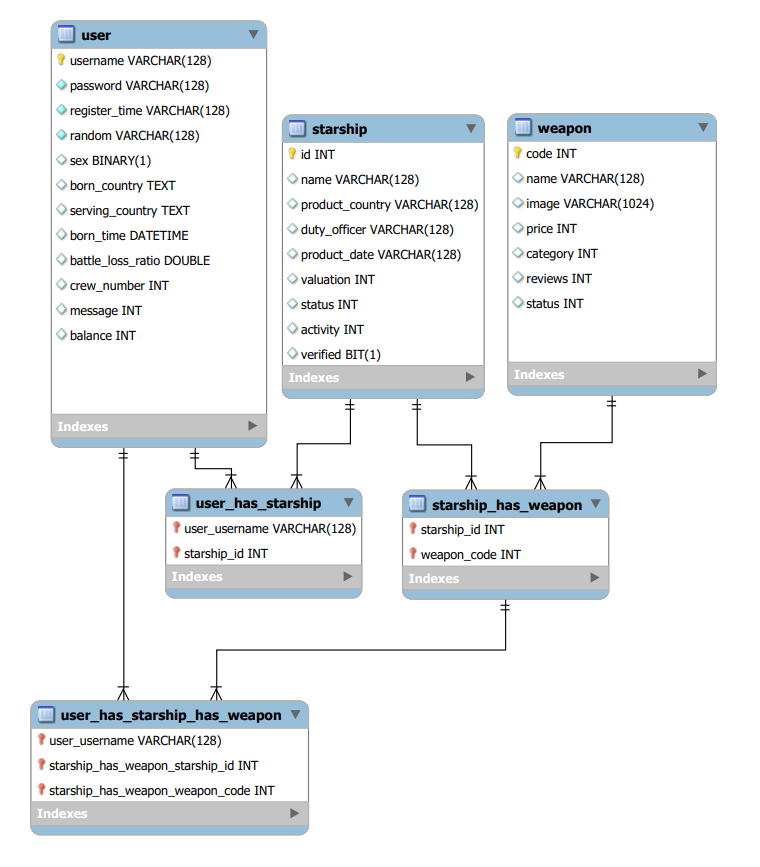
\includegraphics[width=\linewidth]{images/DatabaseSchema}
	\caption{数据库模式 ER 图}
	\label{fig:databaseschema}
\end{figure}


\subsubsection{用户信息管理模块}

用户注册时,系统会将用户信息存储到数据库中,为后续的用户登录和管理提供数据支持。
用户信息管理模块需要调用注册模块提供的用户数据,进行用户信息的显示和修改。用户登录成功后,系统会生成一个会话令牌,用于标识当前登录的用户,并在用户访问其他模块时进行身份验证。

星舰管理模块和武器管理模块需要在用户登录后才能访问,因此这些模块都会依赖于用户登录模块提供的身份验证功能。

用户注销后,系统会清除会话令牌,确保用户退出系统,防止未授权访问。
注销后,用户将无法再访问其他管理模块,确保系统的安全性。
\subsubsection{星舰管理模块}

用户新增星舰信息时,系统会将星舰信息存储到数据库中。武器管理模块需要读取星舰信息,以便在新增或修改武器时能够关联到特定的星舰。

用户修改星舰信息时,系统会更新数据库中的星舰信息。
如果武器管理模块中已有武器关联了被修改的星舰信息,系统会同步更新相关联的武器信息,保持数据一致性。

用户删除星舰信息时,系统会从数据库中删除对应的星舰记录。如果有武器关联了被删除的星舰,系统需要提示用户并处理这些关联,防止数据残留或不一致。

用户可以查看星舰的详细信息,系统会从数据库中读取星舰信息并展示给用户。武器管理模块可以调用查看星舰功能,显示武器所关联的星舰详细信息。

\subsubsection{武器管理模块}

用户新增武器信息时,系统会将武器信息存储到数据库中,并允许用户关联特定的星舰。
星舰管理模块需要提供星舰数据,供用户在新增武器时进行选择。

用户修改武器信息时,系统会更新数据库中的武器信息。如果武器信息中的星舰关联发生变化,系统需要同步更新相关的星舰数据。

用户删除武器信息时,系统会从数据库中删除对应的武器记录。系统需要确保删除武器时,相关的星舰信息和其他模块数据的一致性。


用户可以查看武器的详细信息,系统会从数据库中读取武器信息并展示给用户。星舰管理模块可以调用查看武器功能,显示星舰所装备的武器详细信息。

\subsubsection{用户信息管理模块}

用户可以查看自己的个人信息,系统会从数据库中读取用户数据并展示。用户登录与注册模块提供的用户数据是用户信息管理模块显示和处理的基础。

用户可以修改自己的个人信息,系统会更新数据库中的用户数据。用户登录与注册模块提供的用户数据需要与修改后的用户信息保持一致。

用户可以查看其他用户的公开信息,系统会从数据库中读取公开的用户数据并展示。用户信息管理模块需要确保用户数据的隐私性,避免未经授权的访问。


\subsection{数据库设计}

\subsubsection{数据模型与数据结构}
在星舰管理系统中,数据模型设计围绕用户、星舰、武器及其关系展开。以下是各个实体的详细数据模型:
% Please add the following required packages to your document preamble:
% \usepackage{booktabs}
\begin{table}[H]
	\centering
	\caption{用户数据模型}
	\begin{tabular}{@{}ccc@{}}
		\toprule
		字段                  & 含义   & 类型             \\ \midrule
		username            & 用户名  & (VARCHAR(128)) \\
		password            & 密码   & (VARCHAR(128)) \\
		register\_time      & 注册时间 & (VARCHAR(128)) \\
		random              & 随机码  & (VARCHAR(128)) \\
		sex                 & 性别   & (BINARY(1))    \\
		born\_country       & 出生国家 & (TEXT)         \\
		serving\_country    & 服役国家 & (TEXT)         \\
		born\_time          & 出生时间 & (DATETIME)     \\
		battle\_loss\_ratio & 战损比  & (DOUBLE)       \\
		crew\_number        & 船员数量 & (INT)          \\
		message             & 信息   & (TEXT)         \\
		balance             & 余额   & (INT)          \\ \bottomrule
	\end{tabular}
\end{table}

% Please add the following required packages to your document preamble:
% \usepackage{booktabs}
\begin{table}[H]
	\centering
	\caption{星舰数据模型}
	\begin{tabular}{@{}ccc@{}}
		\toprule
		字段               & 含义   & 类型             \\ \midrule
		id               & 星舰ID & (INT)          \\
		name             & 名称   & (VARCHAR(128)) \\
		product\_country & 生产国家 & (VARCHAR(128)) \\
		duty\_officer    & 值班官员 & (VARCHAR(128)) \\
		product\_date    & 生产日期 & (VARCHAR(128)) \\
		valuation        & 估值   & (INT)          \\
		status           & 状态   & (INT)          \\
		activity         & 活动   & (INT)          \\
		verified         & 验证   & (BIT(1))      \\ \bottomrule
	\end{tabular}
\end{table}


% Please add the following required packages to your document preamble:
% \usepackage{booktabs}
\begin{table}[H]
		\centering
	\caption{武器数据模型}
	\begin{tabular}{@{}ccc@{}}
		\toprule
		字段       & 含义   & 类型              \\ \midrule
		code     & 武器代码 & (INT)           \\
		name     & 名称   & (VARCHAR(128))  \\
		image    & 图片   & (VARCHAR(1024)) \\
		price    & 价格   & (INT)           \\
		category & 类别   & (INT)           \\
		reviews  & 评论   & (INT)           \\
		status   & 状态   & (INT)           \\ \bottomrule
	\end{tabular}
\end{table}

% Please add the following required packages to your document preamble:
% \usepackage{booktabs}
\begin{table}[H]
			\centering
	\caption{用户 - 星舰关系数据模型}
	\begin{tabular}{@{}ccc@{}}
		\toprule
		字段            & 含义   & 类型             \\ \midrule
		ser\_username & 用户名  & (VARCHAR(128)) \\
		starship\_id  & 星舰ID & (INT)          \\ \bottomrule
	\end{tabular}
\end{table}

% Please add the following required packages to your document preamble:
% \usepackage{booktabs}
\begin{table}[H]
	\centering
	\caption{星舰 - 武器关系}
	\begin{tabular}{@{}ccc@{}}
		\toprule
		字段           & 含义   & 类型    \\ \midrule
		starship\_id & 星舰ID & (INT) \\
		weapon\_code & 武器代码 & (INT) \\ \bottomrule
	\end{tabular}
\end{table}

% Please add the following required packages to your document preamble:
% \usepackage{booktabs}
\begin{table}[H]
		\centering
	\caption{用户 - 星舰 - 武器关系}
	\begin{tabular}{@{}ccc@{}}
		\toprule
		字段                                                      & 含义                       & 类型                        \\ \midrule
		user\_username                                          & 用户名                      & (VARCHAR(128))            \\
		starship\_has\_weapon\_starship\_id                     & 星舰ID                     & (INT)                     \\
		starship\_has\_weapon\_weapon\_code & 武器代码 & (INT) \\ \bottomrule
	\end{tabular}
\end{table}

数据结构设计确保了各实体及其关系的清晰定义和高效操作。用户 (user) 表存储用户信息,主要字段为用户名、密码、注册时间等;星舰 (starship) 表存储星舰信息,主要字段为星舰ID、名称、生产国家等。武器 (weapon) 表存储武器信息,主要字段为武器代码、名称、图片等。用户-星舰关系 (user\_has\_starship) 表存储用户和星舰的多对多关系。星舰-武器关系 (starship\_has\_weapon) 表存储星舰和武器的多对多关系。用户-星舰-武器关系 (user\_has\_starship\_has\_weapon) 表存储用户、星舰和武器的多对多对多关系。

\subsubsection{数据存储与访问策略}

我使用分表存储,将用户、星舰、武器及其关系分别存储在不同的表中,确保数据存储的结构化和模块化。利用索引优化在各表的关键字段上建立索引(例如 username, id, code),提高数据查询效率。数据完整性通过外键约束(例如 user\_has\_starship 表中的 user\_username 和 starship\_id),确保数据的一致性和完整性。

访问策略有如下内容:

\begin{enumerate}
	\item CRUD 操作
	\begin{itemize}
		\item \textbf{创建 (Create)}:使用 INSERT 语句将新数据插入到相关表中。
		\item \textbf{读取 (Read)}:使用 SELECT 语句从表中检索数据,根据查询条件(例如 WHERE 子句)获取所需信息。
		\item \textbf{更新 (Update)}:使用 UPDATE 语句修改表中已有的数据,确保数据的实时性和准确性。
		\item \textbf{删除 (Delete)}:使用 DELETE 语句从表中移除不再需要的数据,保持数据库的简洁。
	\end{itemize}
	
	\item 利用 SQL 的 JOIN 操作,通过关联表实现跨表查询,例如查询用户的星舰信息或星舰的武器信息。
	
	\item 对于频繁访问的数据,可以考虑引入缓存机制(如 Redis),提高数据访问的效率和系统的响应速度。
	
	\item 对于大量数据的查询,使用分页技术(如 LIMIT 和 OFFSET)控制每次查询的数据量,提高查询效率和用户体验。
	
\end{enumerate}




\section{详细设计}
开发时我先开发了前端,然后根据前端的开发需求开发了后端,这种开发顺序有以下好处:

\begin{enumerate}
	\item 前端开发通常涉及用户界面的设计和用户交互的实现。先开发前端可以确保用户体验(UI/UX)优先,使得开发团队可以更早地进行用户测试和反馈收集,进而优化用户体验。
	\item 通过快速构建前端原型,可以帮助设计团队和业务方确认和调整需求。这样可以在正式开发之前发现和解决问题,避免后期大规模返工。
	\item 前端开发过程中会明确需要的 API 接口和数据格式,这可以帮助后端开发人员更有针对性地设计和实现API。前端开发可以驱动 API 设计,确保后端提供的数据和功能完全符合前端需求。
\end{enumerate}

因此,本文在介绍具体设计时,也按照先前端、再后端的顺序来介绍。

\subsection{前端详细设计}

前端主要技术栈如图 \ref{fig:frontend} 所示。

% TODO: \usepackage{graphicx} required
\begin{figure}[H]
	\centering
	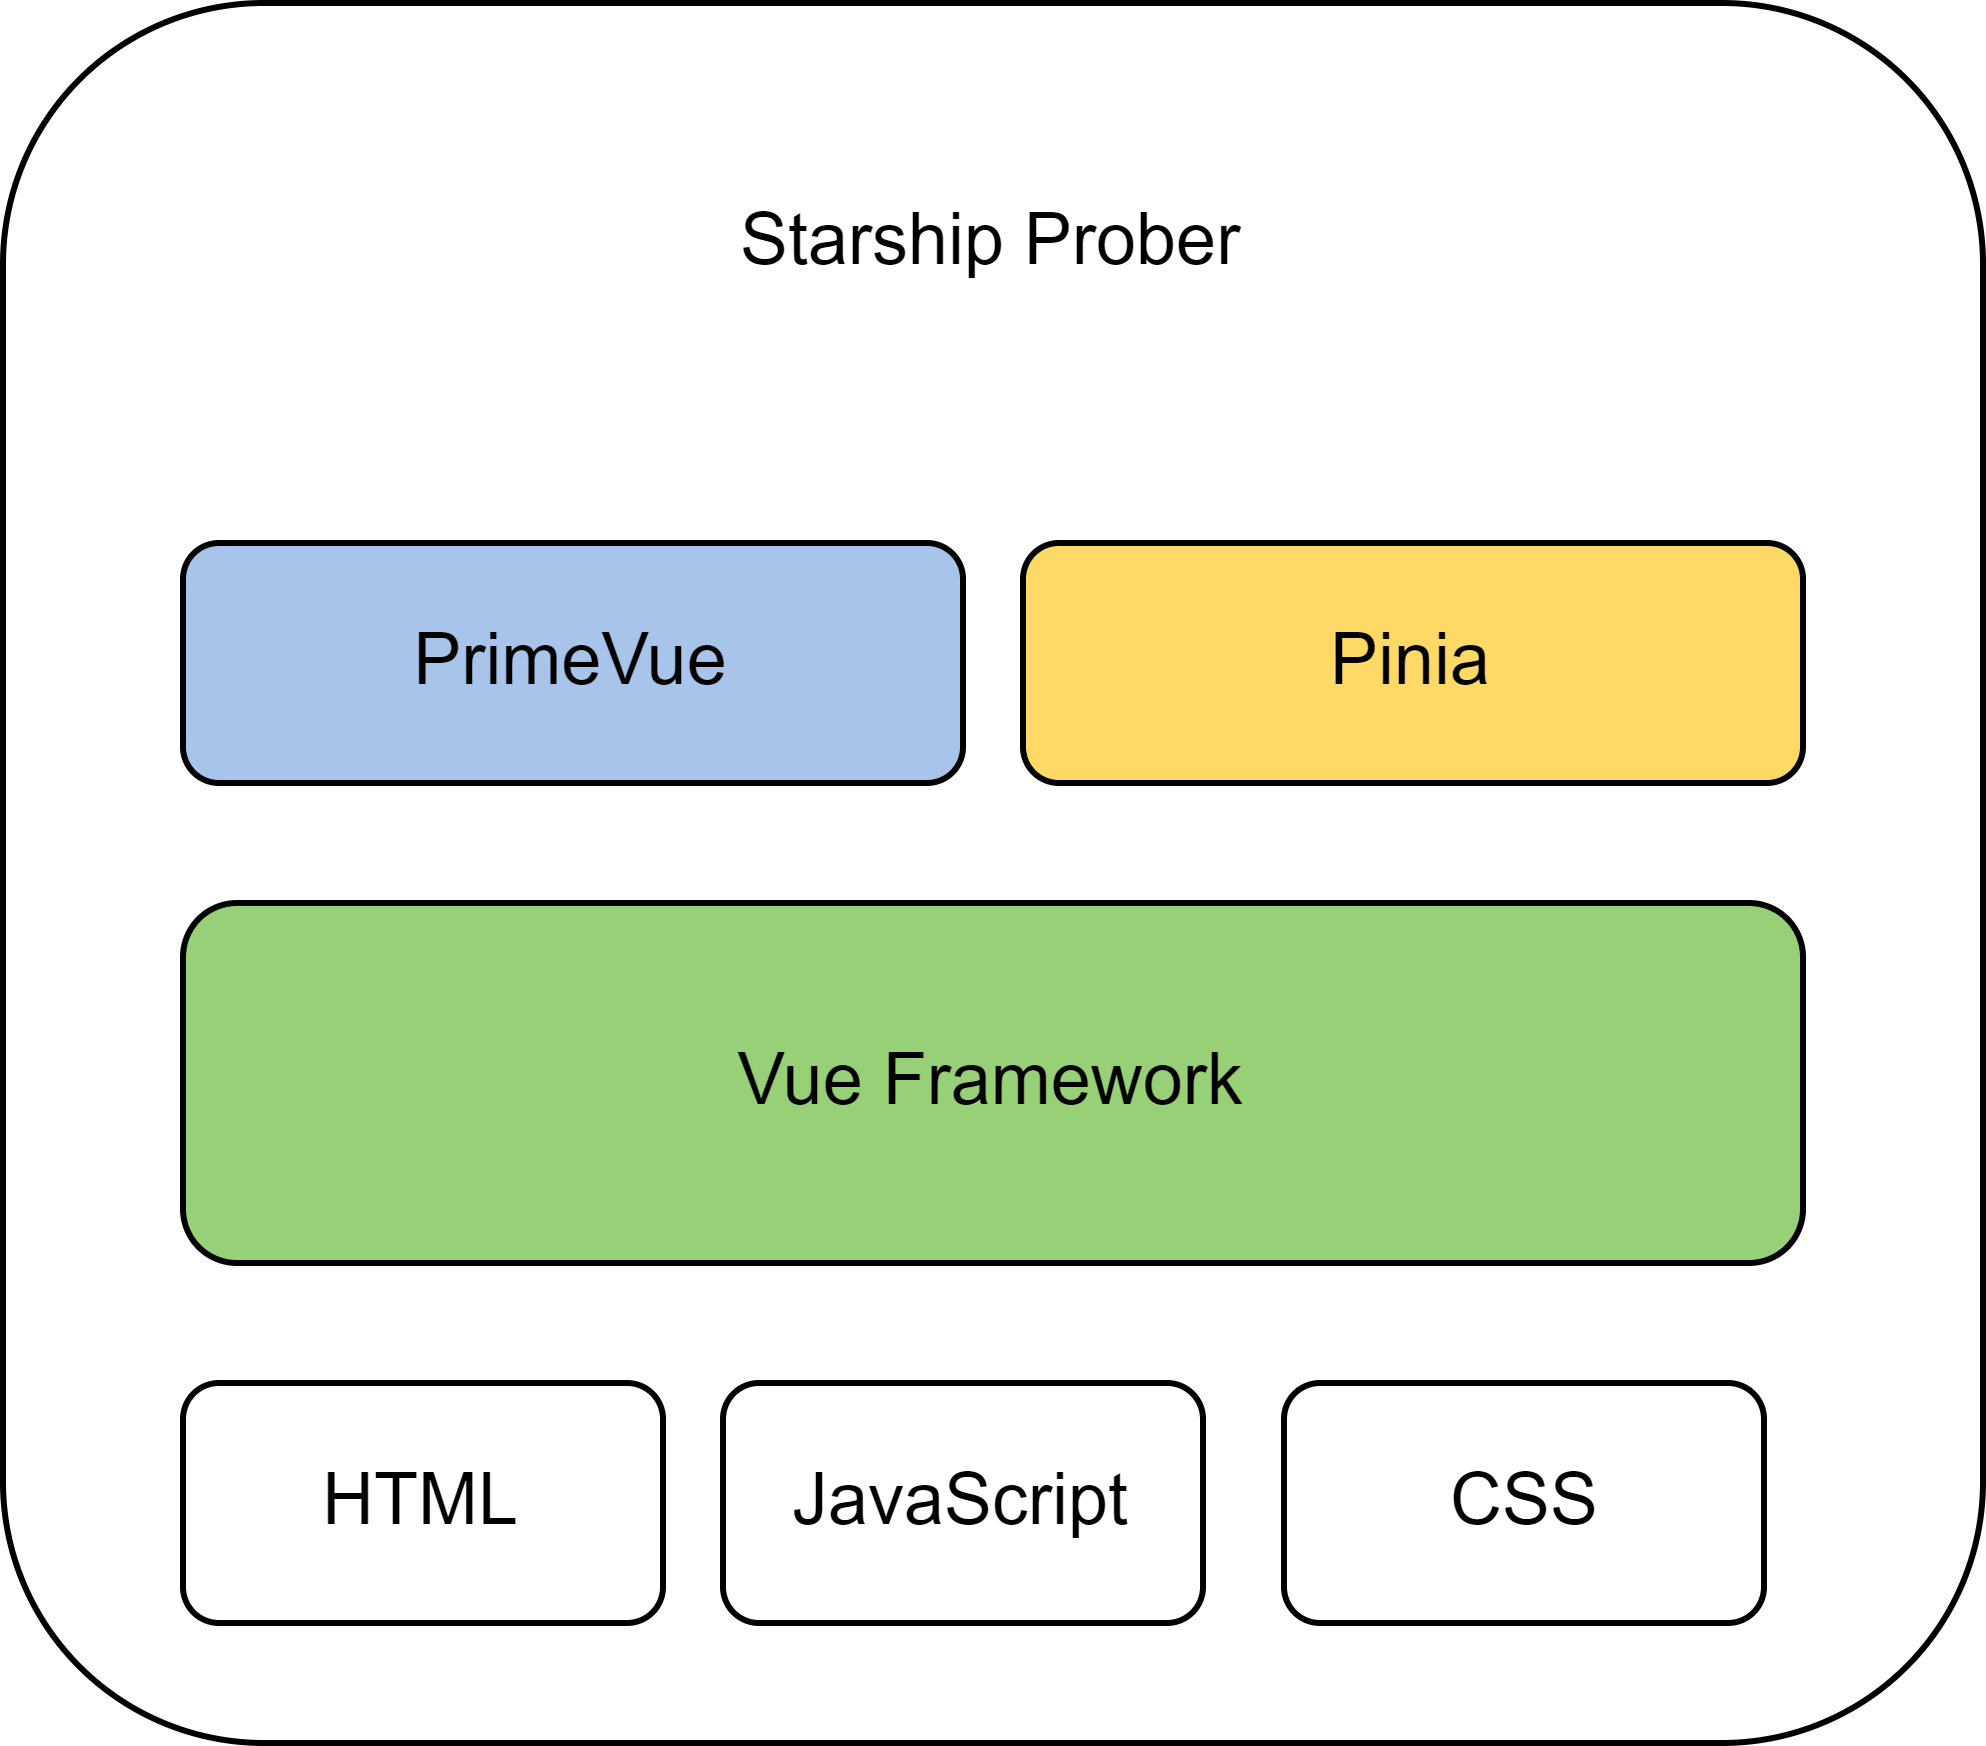
\includegraphics[width=0.7\linewidth]{images/FrontEnd}
	\caption{前端技术栈}
	\label{fig:frontend}
\end{figure}


Pinia 是 Vue.js 的一个状态管理库,它是 Vuex 的下一代替代品。Pinia 的设计目标是提供更简单、更直观的 API,同时保留和提升 Vuex 的功能。Pinia 提供了更加直观和易于使用的 API,使得状态管理变得更加简单和可维护。它支持模块化,可以将状态和逻辑拆分到不同的 store 中,从而使代码更具可读性和可维护性。同时 Pinia 对 TypeScript 有很好的支持,提供了类型安全的状态管理,这对于大型项目尤为重要。其还集成了 Vue DevTools,可以方便地进行状态调试。

% TODO: \usepackage{graphicx} required
\begin{figure}[H]
	\centering
	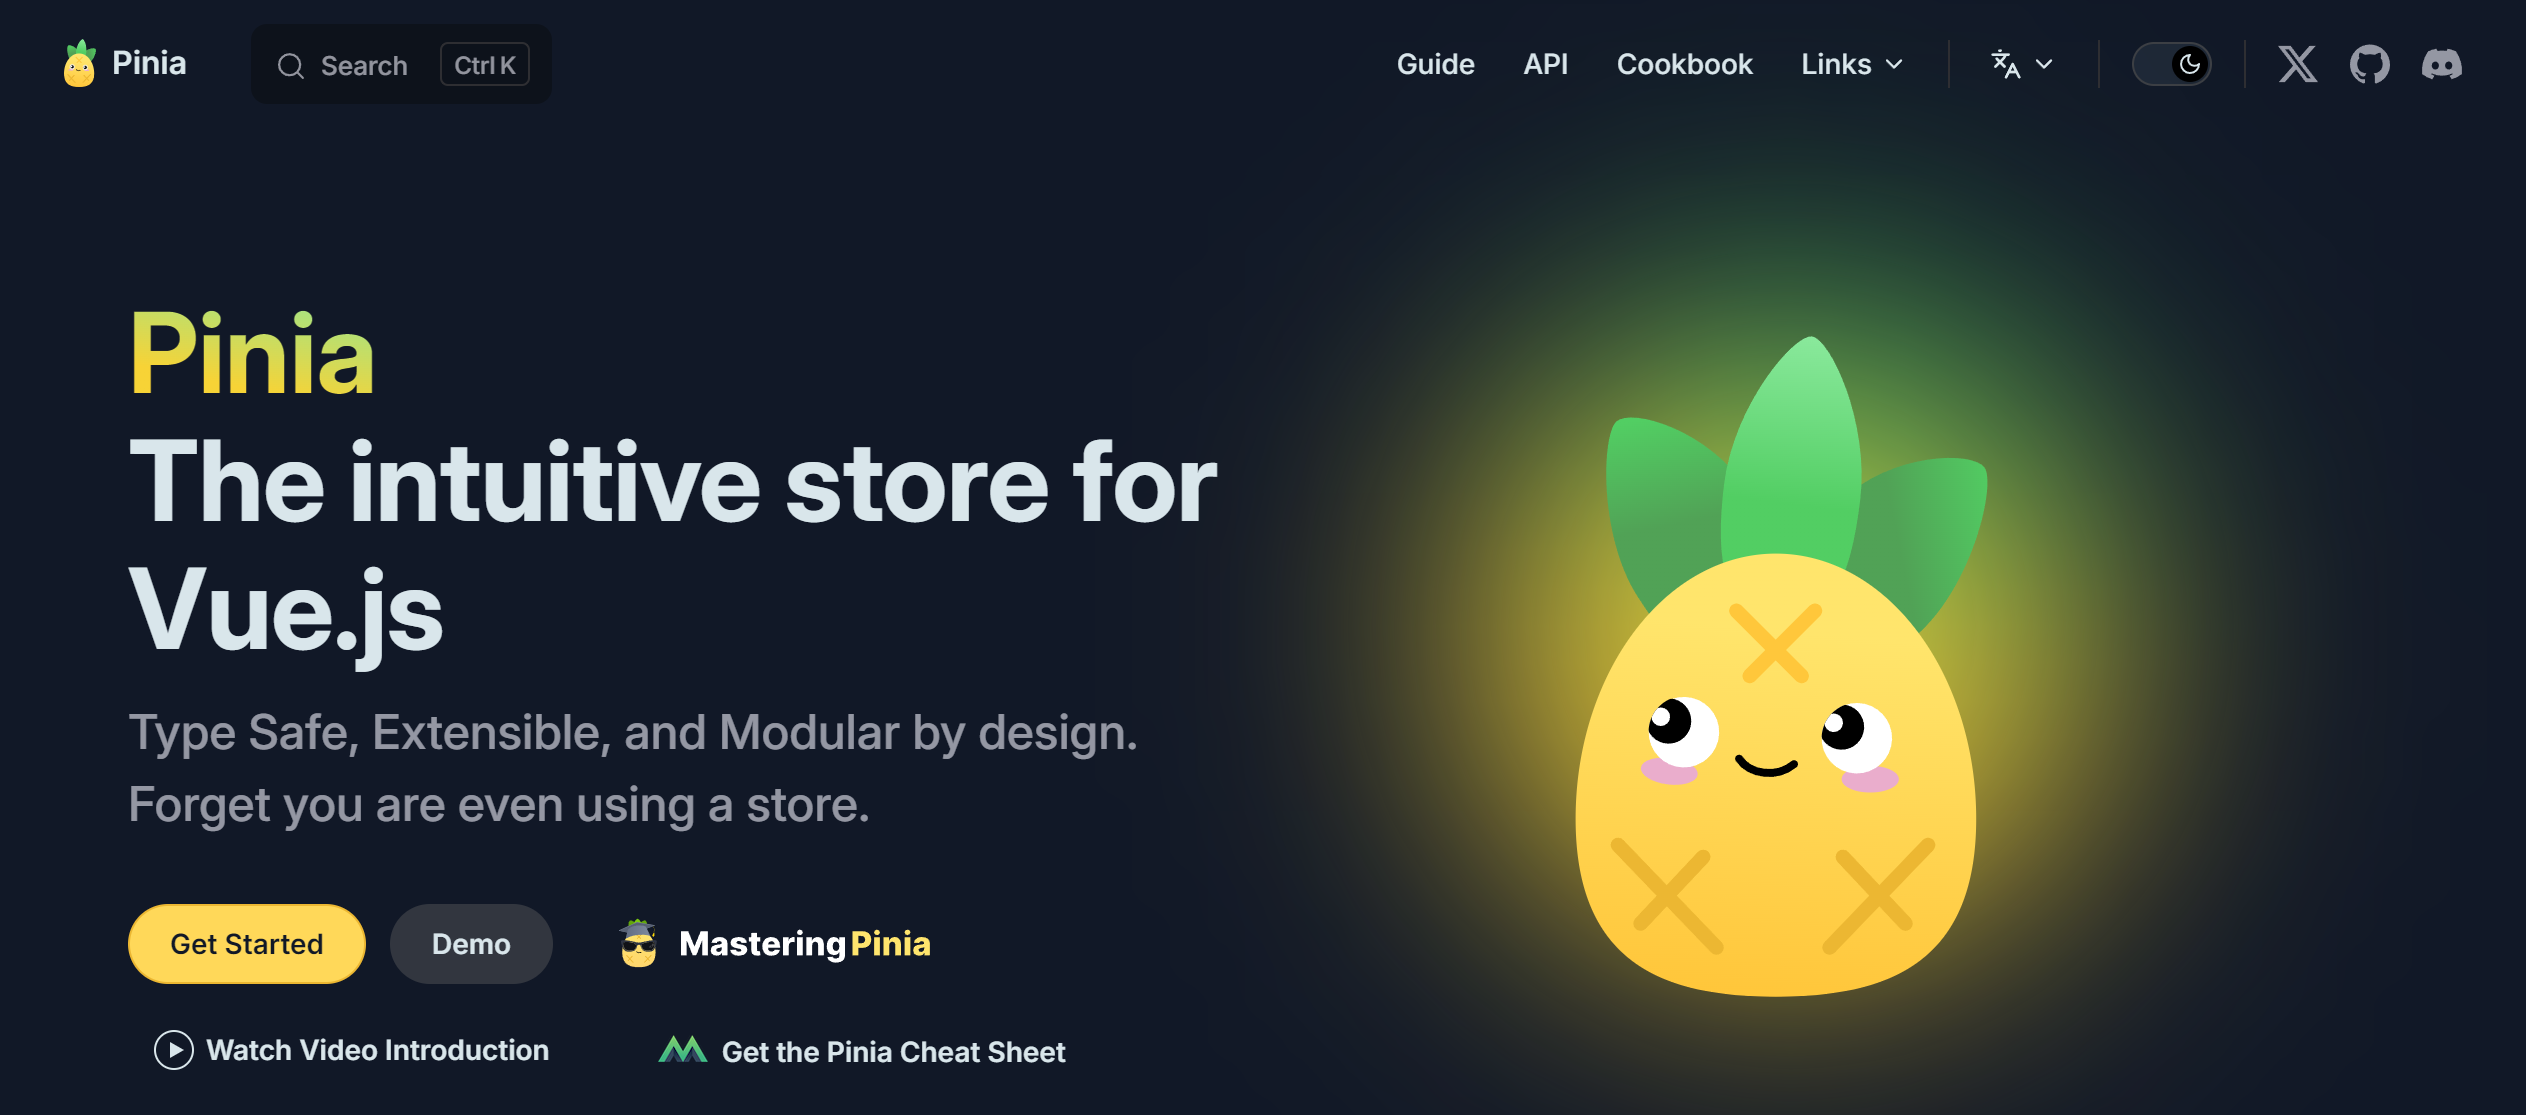
\includegraphics[width=\linewidth]{images/Pinia}
	\caption{Pinia 状态管理插件}
	\label{fig:pinia}
\end{figure}


PrimeVue 是一个用于 Vue.js 的全面 UI 组件库,提供了丰富的 UI 组件集,帮助开发者快速构建高质量的用户界面。PrimeVue 由 PrimeTek 维护,旨在简化前端开发过程,并提供一致且美观的设计。PrimeVue 提供了超过 90 个高质量的 UI 组件,涵盖了表格、表单、按钮、布局等多种常用场景。所有组件都经过优化,确保在不同的设备和屏幕尺寸上具有出色的表现。PrimeVue 支持多种预定义的主题,并允许开发者自定义样式,轻松实现品牌化设计。它还提供了国际化支持,方便开发多语言应用。

% TODO: \usepackage{graphicx} required
\begin{figure}[H]
	\centering
	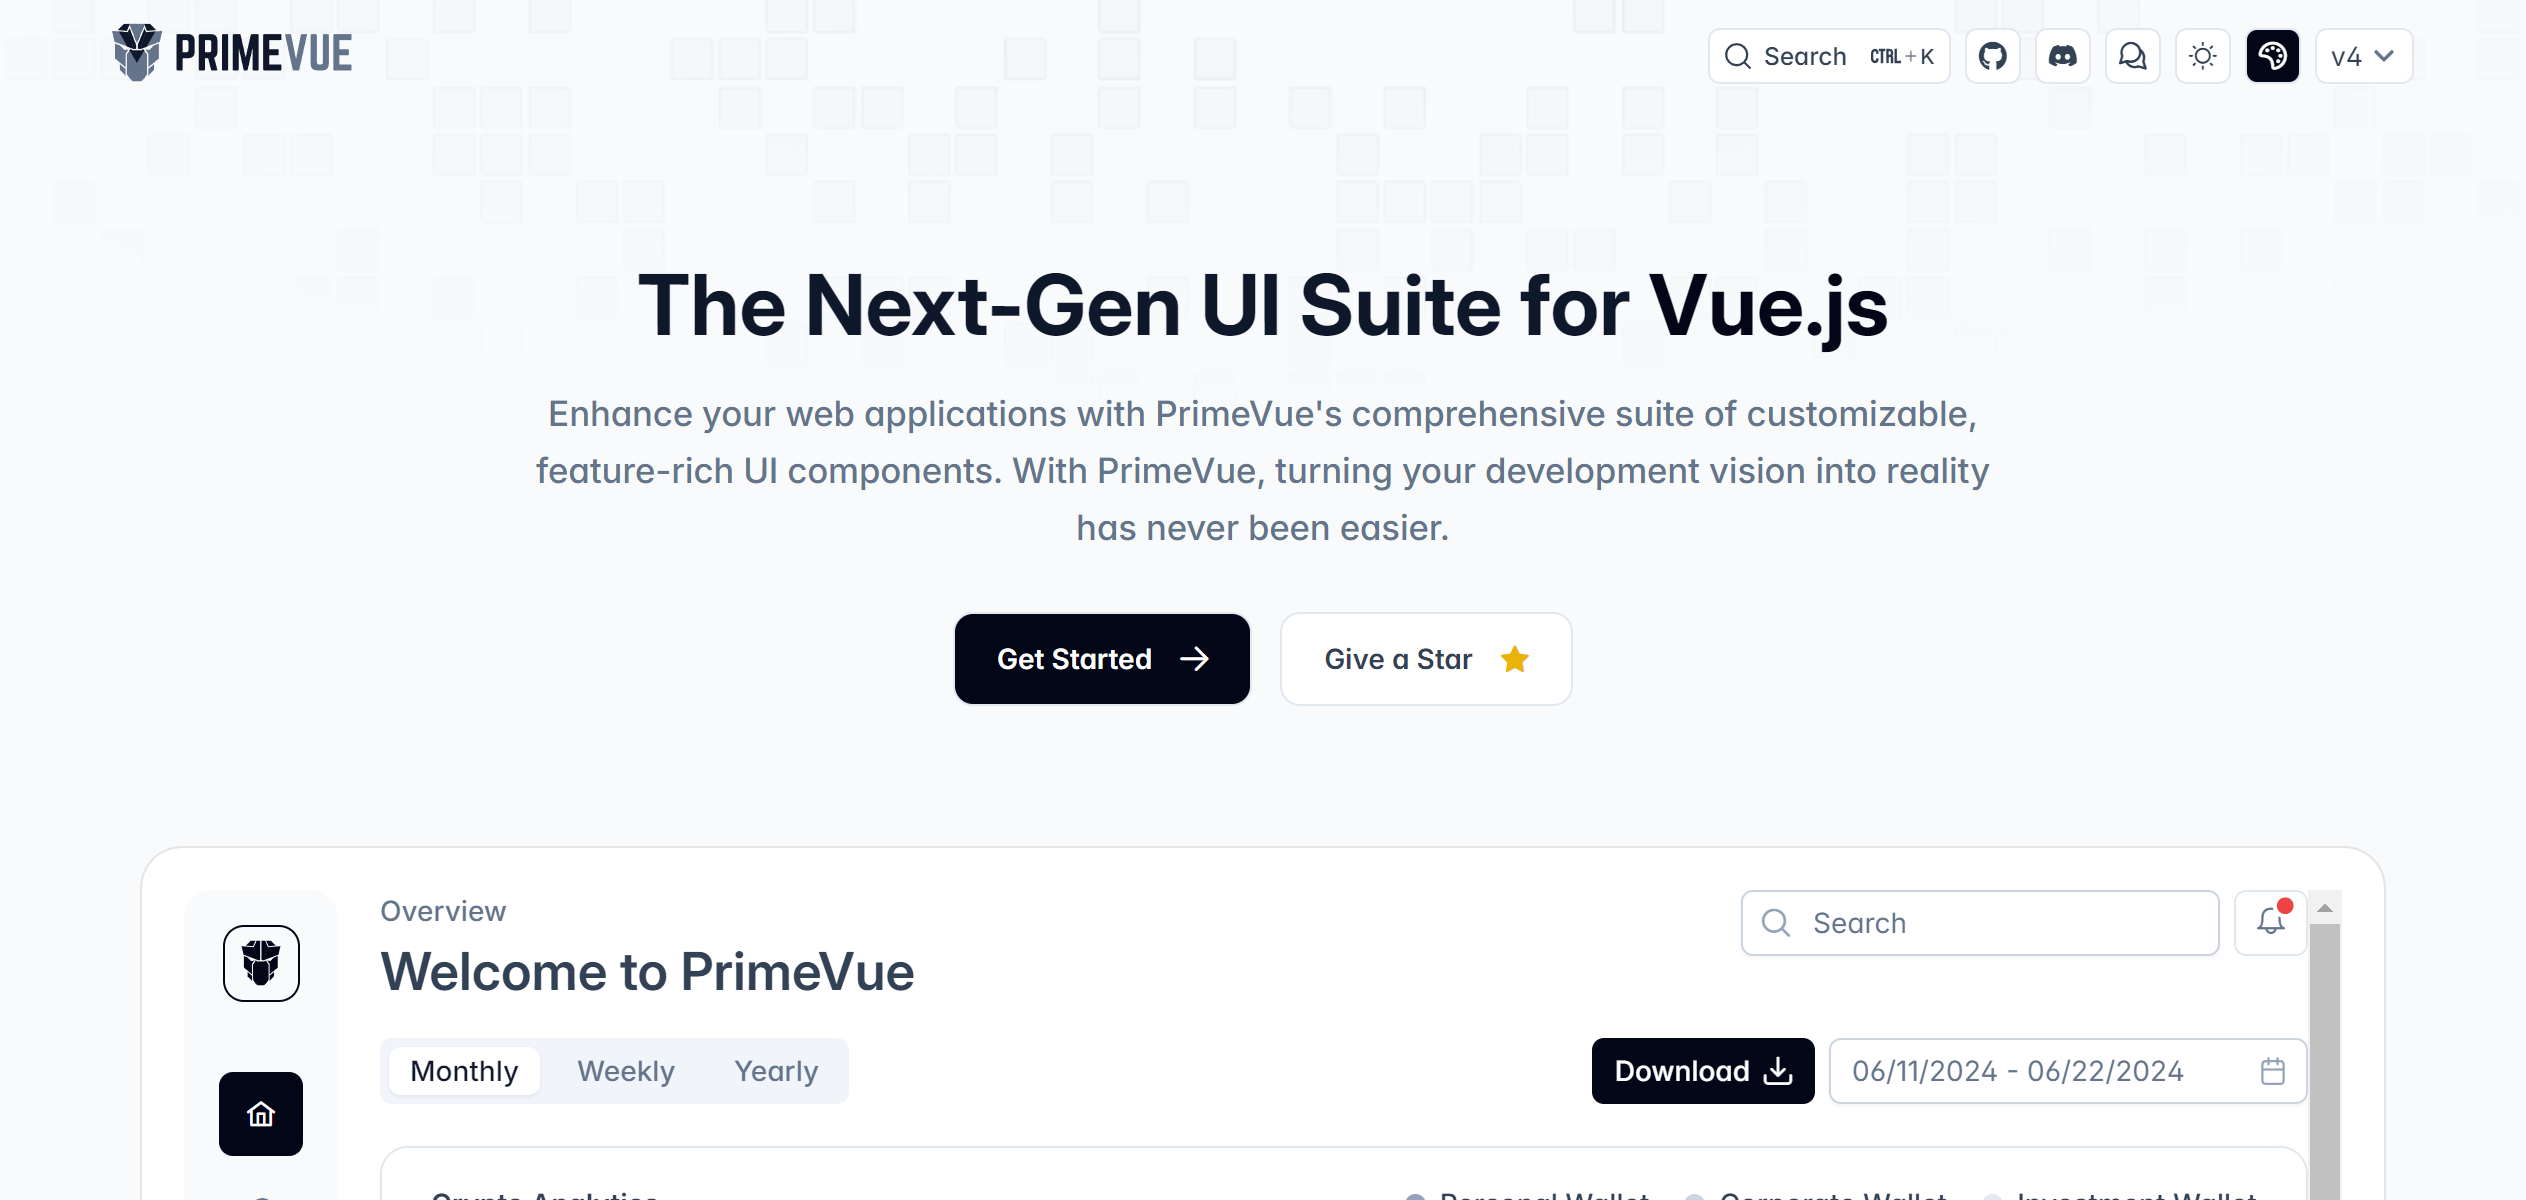
\includegraphics[width=\linewidth]{images/PrimeVue}
	\caption{PrimeVue 主题库}
	\label{fig:primevue}
\end{figure}

\subsubsection{前端页面分级}

% TODO: \usepackage{graphicx} required
\begin{figure}[H]
	\centering
	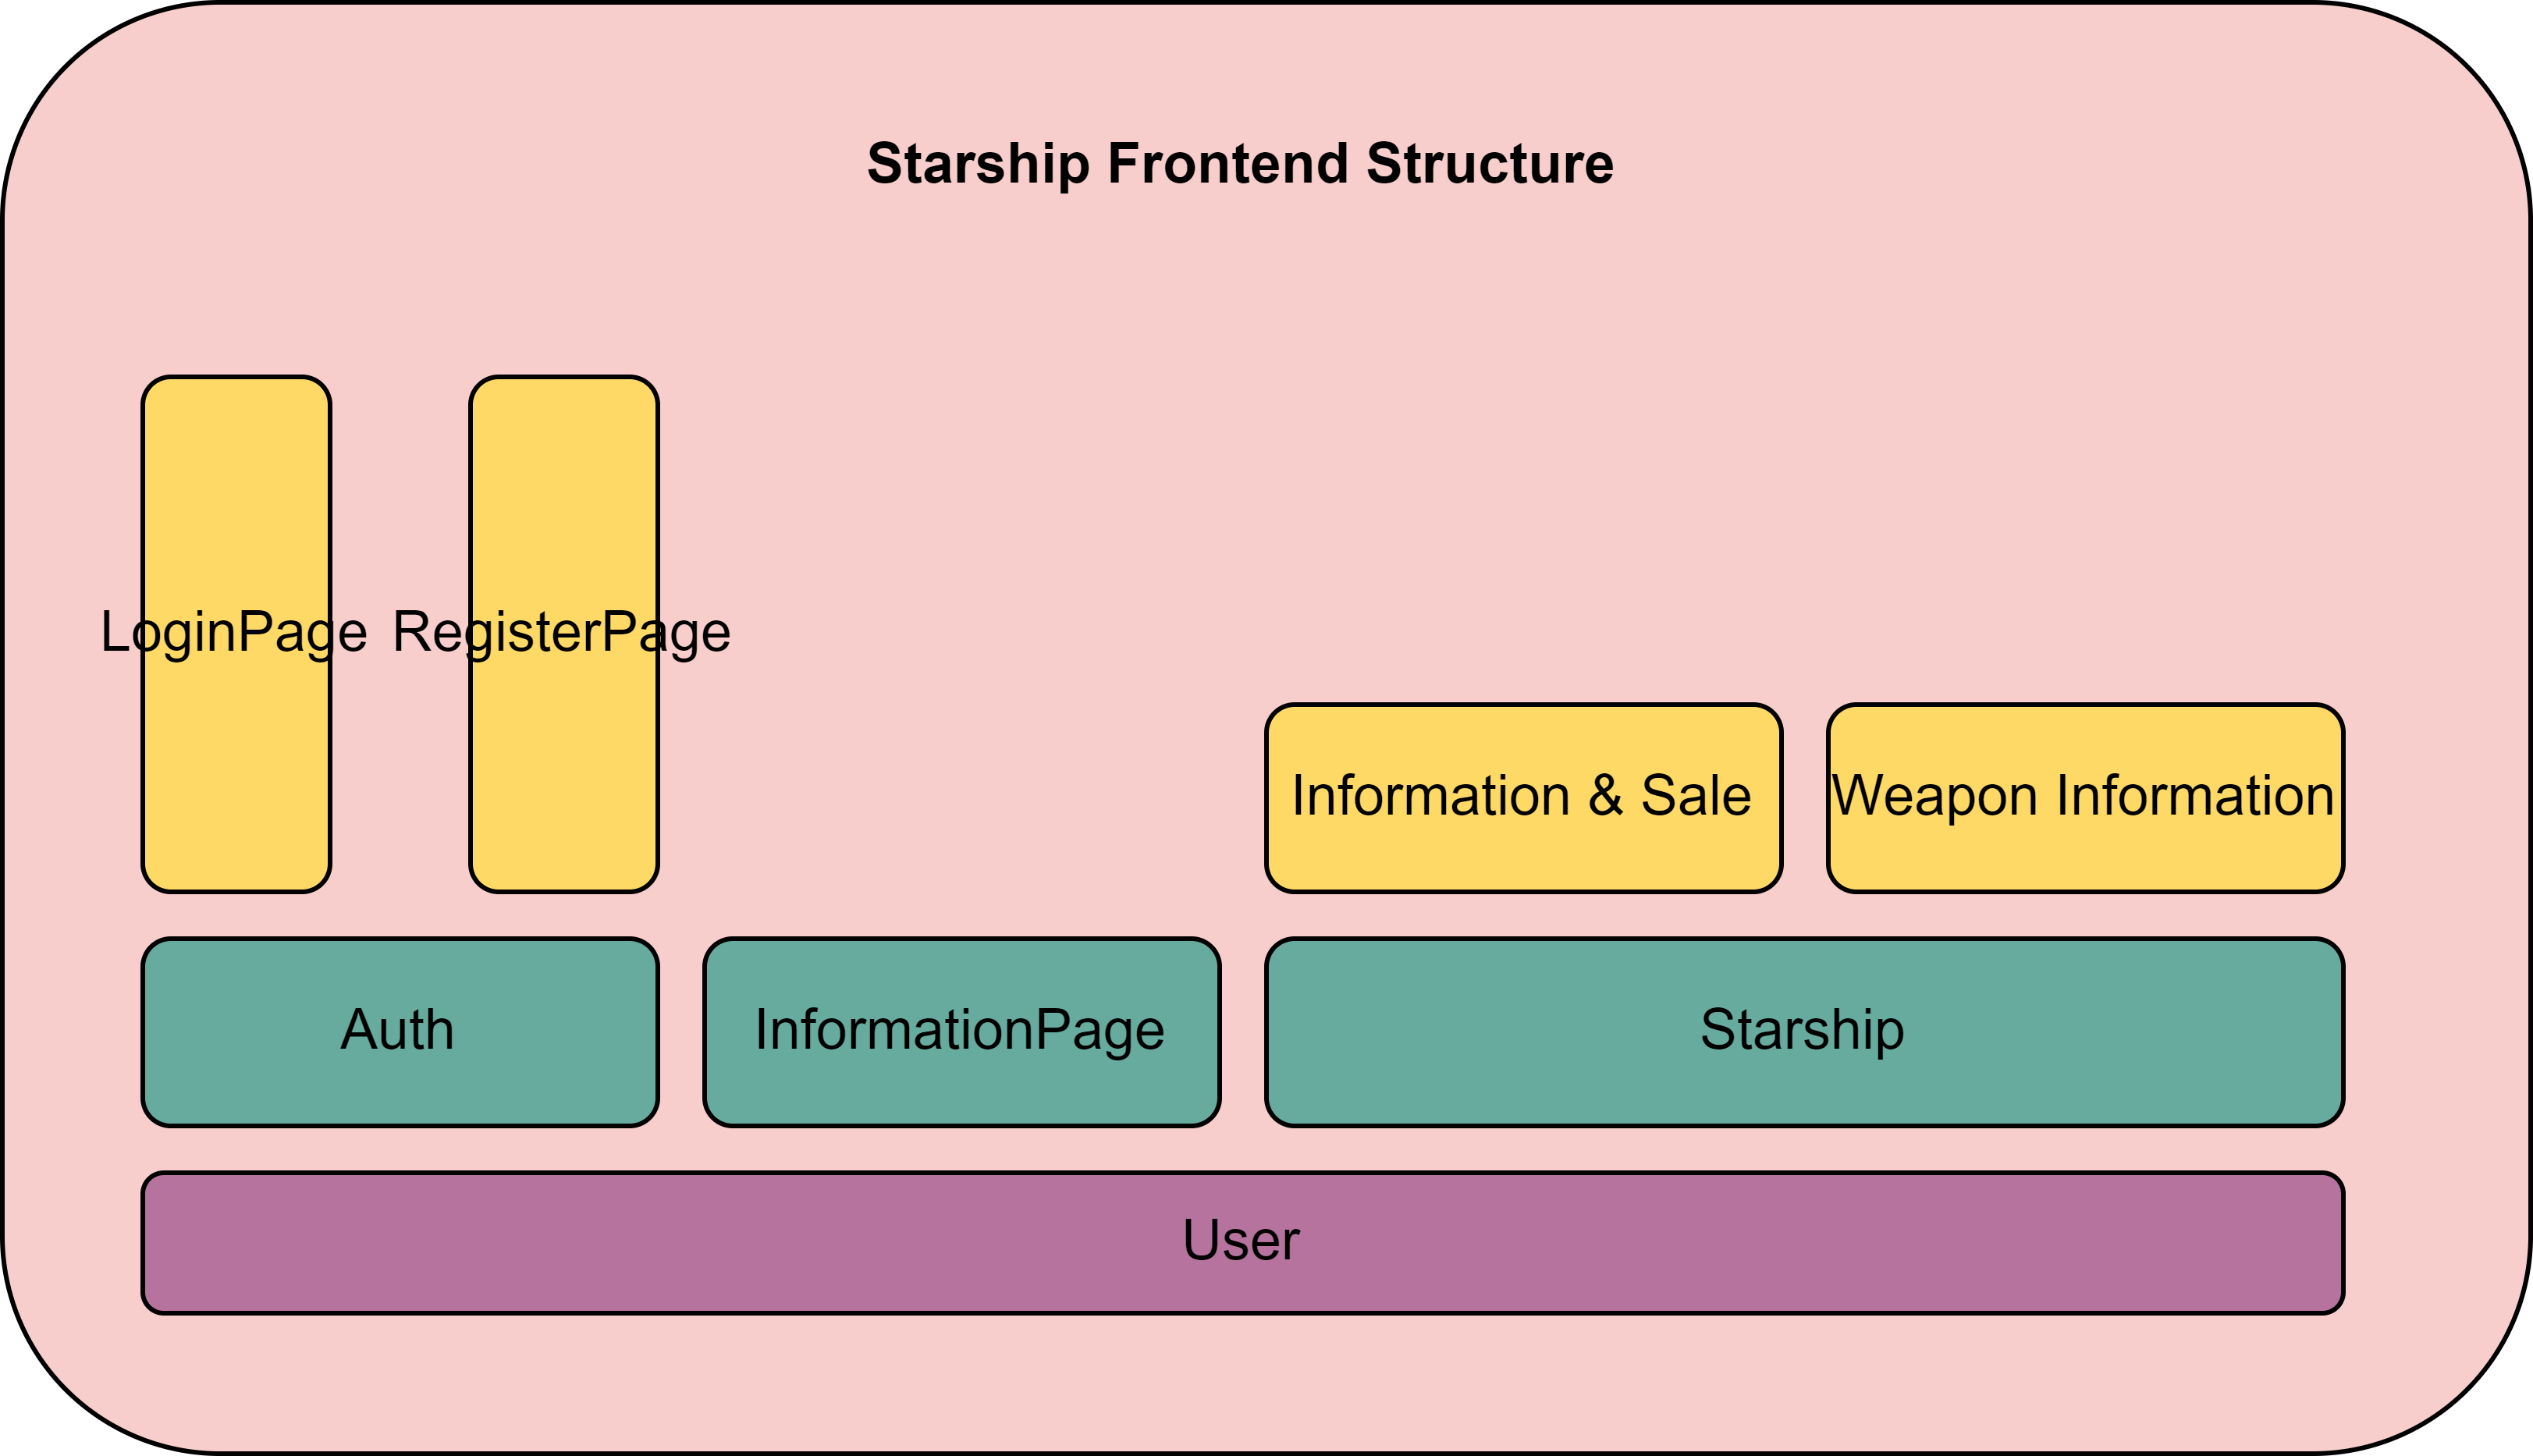
\includegraphics[width=\linewidth]{images/FrontEndPageLayers}
	\caption{前端页面结构设计}
	\label{fig:frontendpagelayers}
\end{figure}

Login Page 和 Register Page 这两个是页面是用户登录和注册的入口点。所有的注册和登录操作都要由这两个页面来完成。Auth 这一层级代表认证(Authentication)功能,用于处理用户的登录、注销等操作,并确保只有经过验证的用户才能访问特定的内容。InformationPage 层级包含有关星舰的信息展示页面,如详细信息、销售数据等。Information \& Sale 层级专门用来展示星舰信息和销售情况的部分。而 Weapon Information 显示与星舰相关的武器信息。Starship 这一层级是星舰的主要内容区域,包括各种子模块或功能。
User 层,也即最底层表示用户层,所有上述的功能都是为了服务于用户而设计的。

\subsubsection{请求与拦截器}

如下是前端使用的拦截器,发送请求时增加上 JWT(Java Web Token) 校验的首部 Authoration 选项,接收请求时验证状态码。

\begin{verbatim}
	import { useTokenStore } from '@/store/token.js';
	import router from '@/router';
	import { useCONST } from '@/config/const';
	
	export const request = async (input, init) => {
		const tokenStore = useTokenStore();
		const CONST = useCONST();
		if (tokenStore?.token === '' && !['/auth/login', '/auth/register']
		.includes(router.currentRoute._value.path)) {
			await router.push('/auth/login');
			throw new Error(CONST.EXCEPTION_TIP);
		}
		
		init.headers = {
			'Content-Type': 'application/x-www-form-urlencoded',
			Authorization: tokenStore.token
		};
		const response = await fetch(input, init);
		switch (response.status) {
			case 401:
			await router.push('/auth/login');
			throw new Error(CONST.EXCEPTION_TIP);
		}
		return response;
	};
	
\end{verbatim}

由于我使用了 Pinia 作为状态管理,故把用户的 JWT 直接借助 Pinia 插件进行存储。实际上我还存储了用户的信息等,这会在后面提到。

JSON Web Token (JWT) 是一种开放标准(RFC 7519),用于在各方之间以安全的方式传输信息。JWT 是一个紧凑且自包含的令牌,它允许信息在各方之间以一种安全且可验证的方式进行传递。JWT 通常被用于身份验证和授权场景中。其主要由三部分组成,通过点号(.)分隔:

\textbf{Header(头部)} 通常包含了令牌类型(typ)和加密算法(alg)。例如:

\begin{verbatim}
	{
		"typ": "JWT",
		"alg": "HS256"
	}
\end{verbatim}

\textbf{Payload(载荷)} 存储在 JWT 中的实际数据,它包含一系列声明(claims)。声明可以是标准的(如 iss 表示发行者,exp 表示过期时间)或自定义的。

\textbf{Signature(签名)} 签名用于确保 JWT 在传输过程中没有被篡改。它是由一个密钥(对称或非对称)和前两部分(Header 和 Payload)组成的,使用指定的算法生成。例如,使用 HMAC SHA-256 算法,签名会这样计算:

\begin{verbatim}
	HMACSHA256(
		base64UrlEncode(header) + "." +
		base64UrlEncode(payload),
	secret)
\end{verbatim}

JWT 的优点在于,服务器不需要保存任何会话状态,因为所有必要信息都存储在 JWT 内,这使得 JWT 非常适合微服务架构和负载均衡环境。JWT 可以轻松地在不同的域之间传递,因为它们是自包含的,不需要依赖于 cookie 或 session。JWT 使用 JSON 格式,因此非常轻量,易于解析和理解。

JWT 也有一些缺点,例如一旦颁发就无法撤销,除非设定一个短的有效期并频繁刷新,或者有额外的机制来管理令牌的有效性。

% TODO: \usepackage{graphicx} required
\begin{figure}[H]
	\centering
	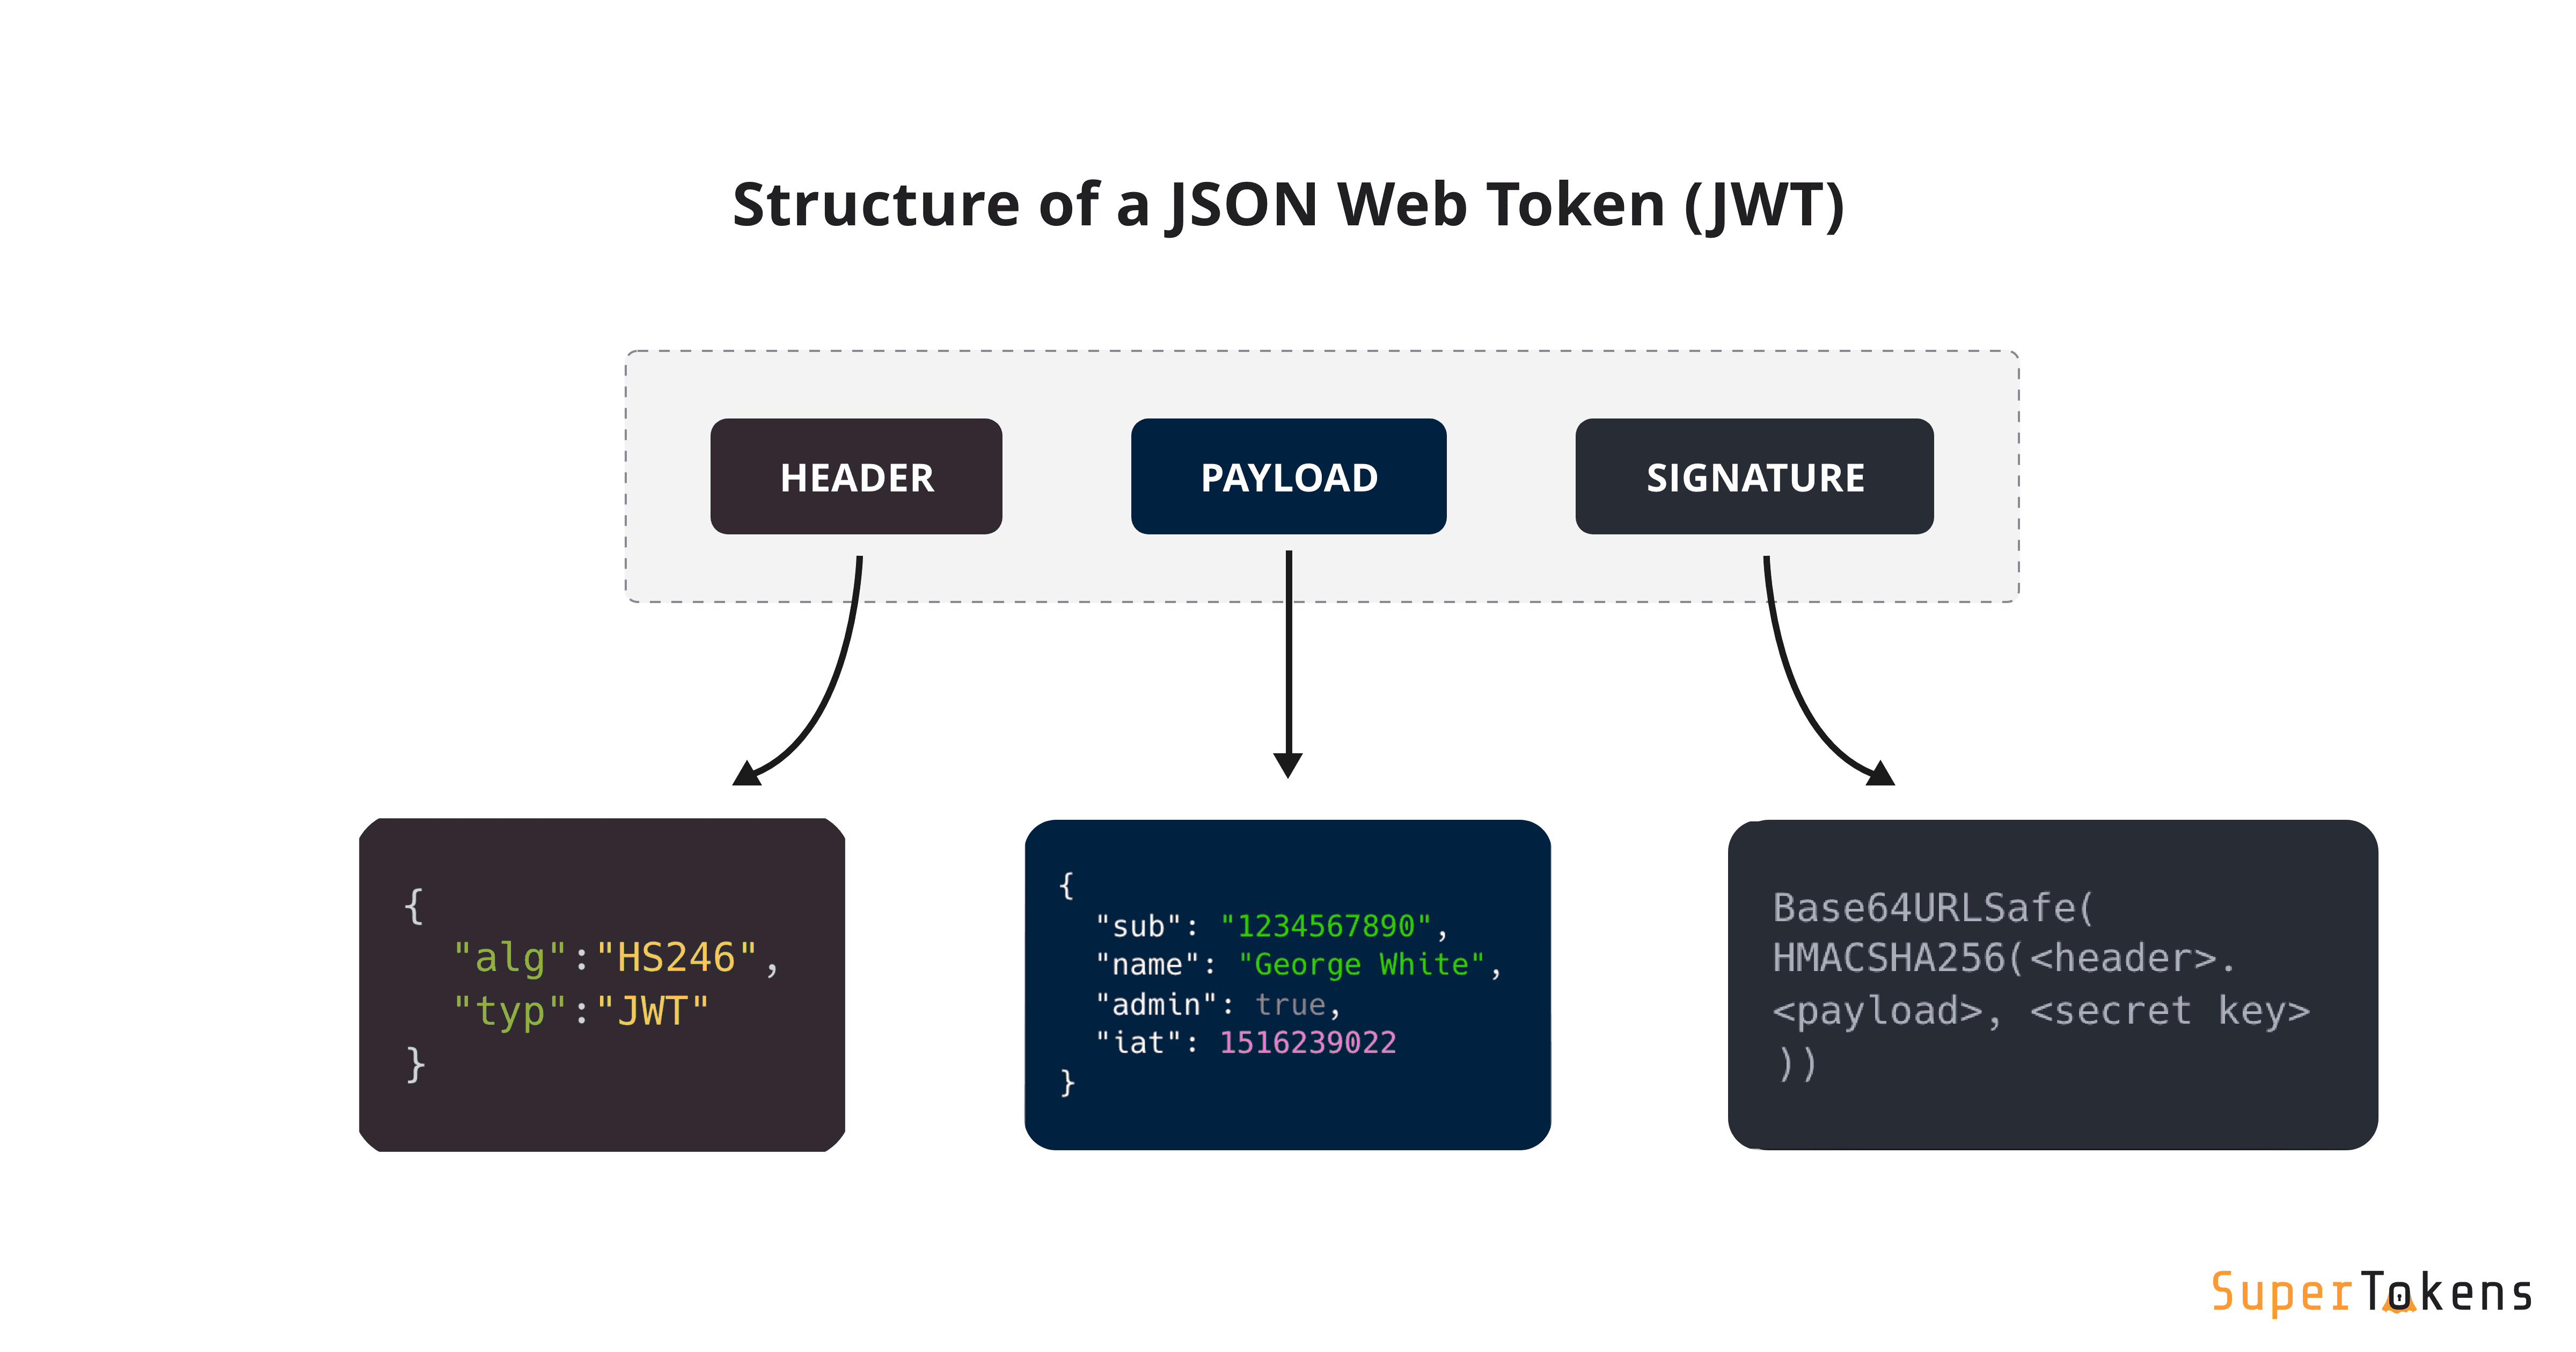
\includegraphics[width=\linewidth]{images/JWT}
	\caption{JWT 的三部分结构}
	\label{fig:jwt}
\end{figure}

\subsubsection{注册与登录}

用户登录界面需要访问 /auth/login 路径,也可以访问 / 路径后重定向到 /auth/login 下。

% TODO: \usepackage{graphicx} required
\begin{figure}[H]
	\centering
	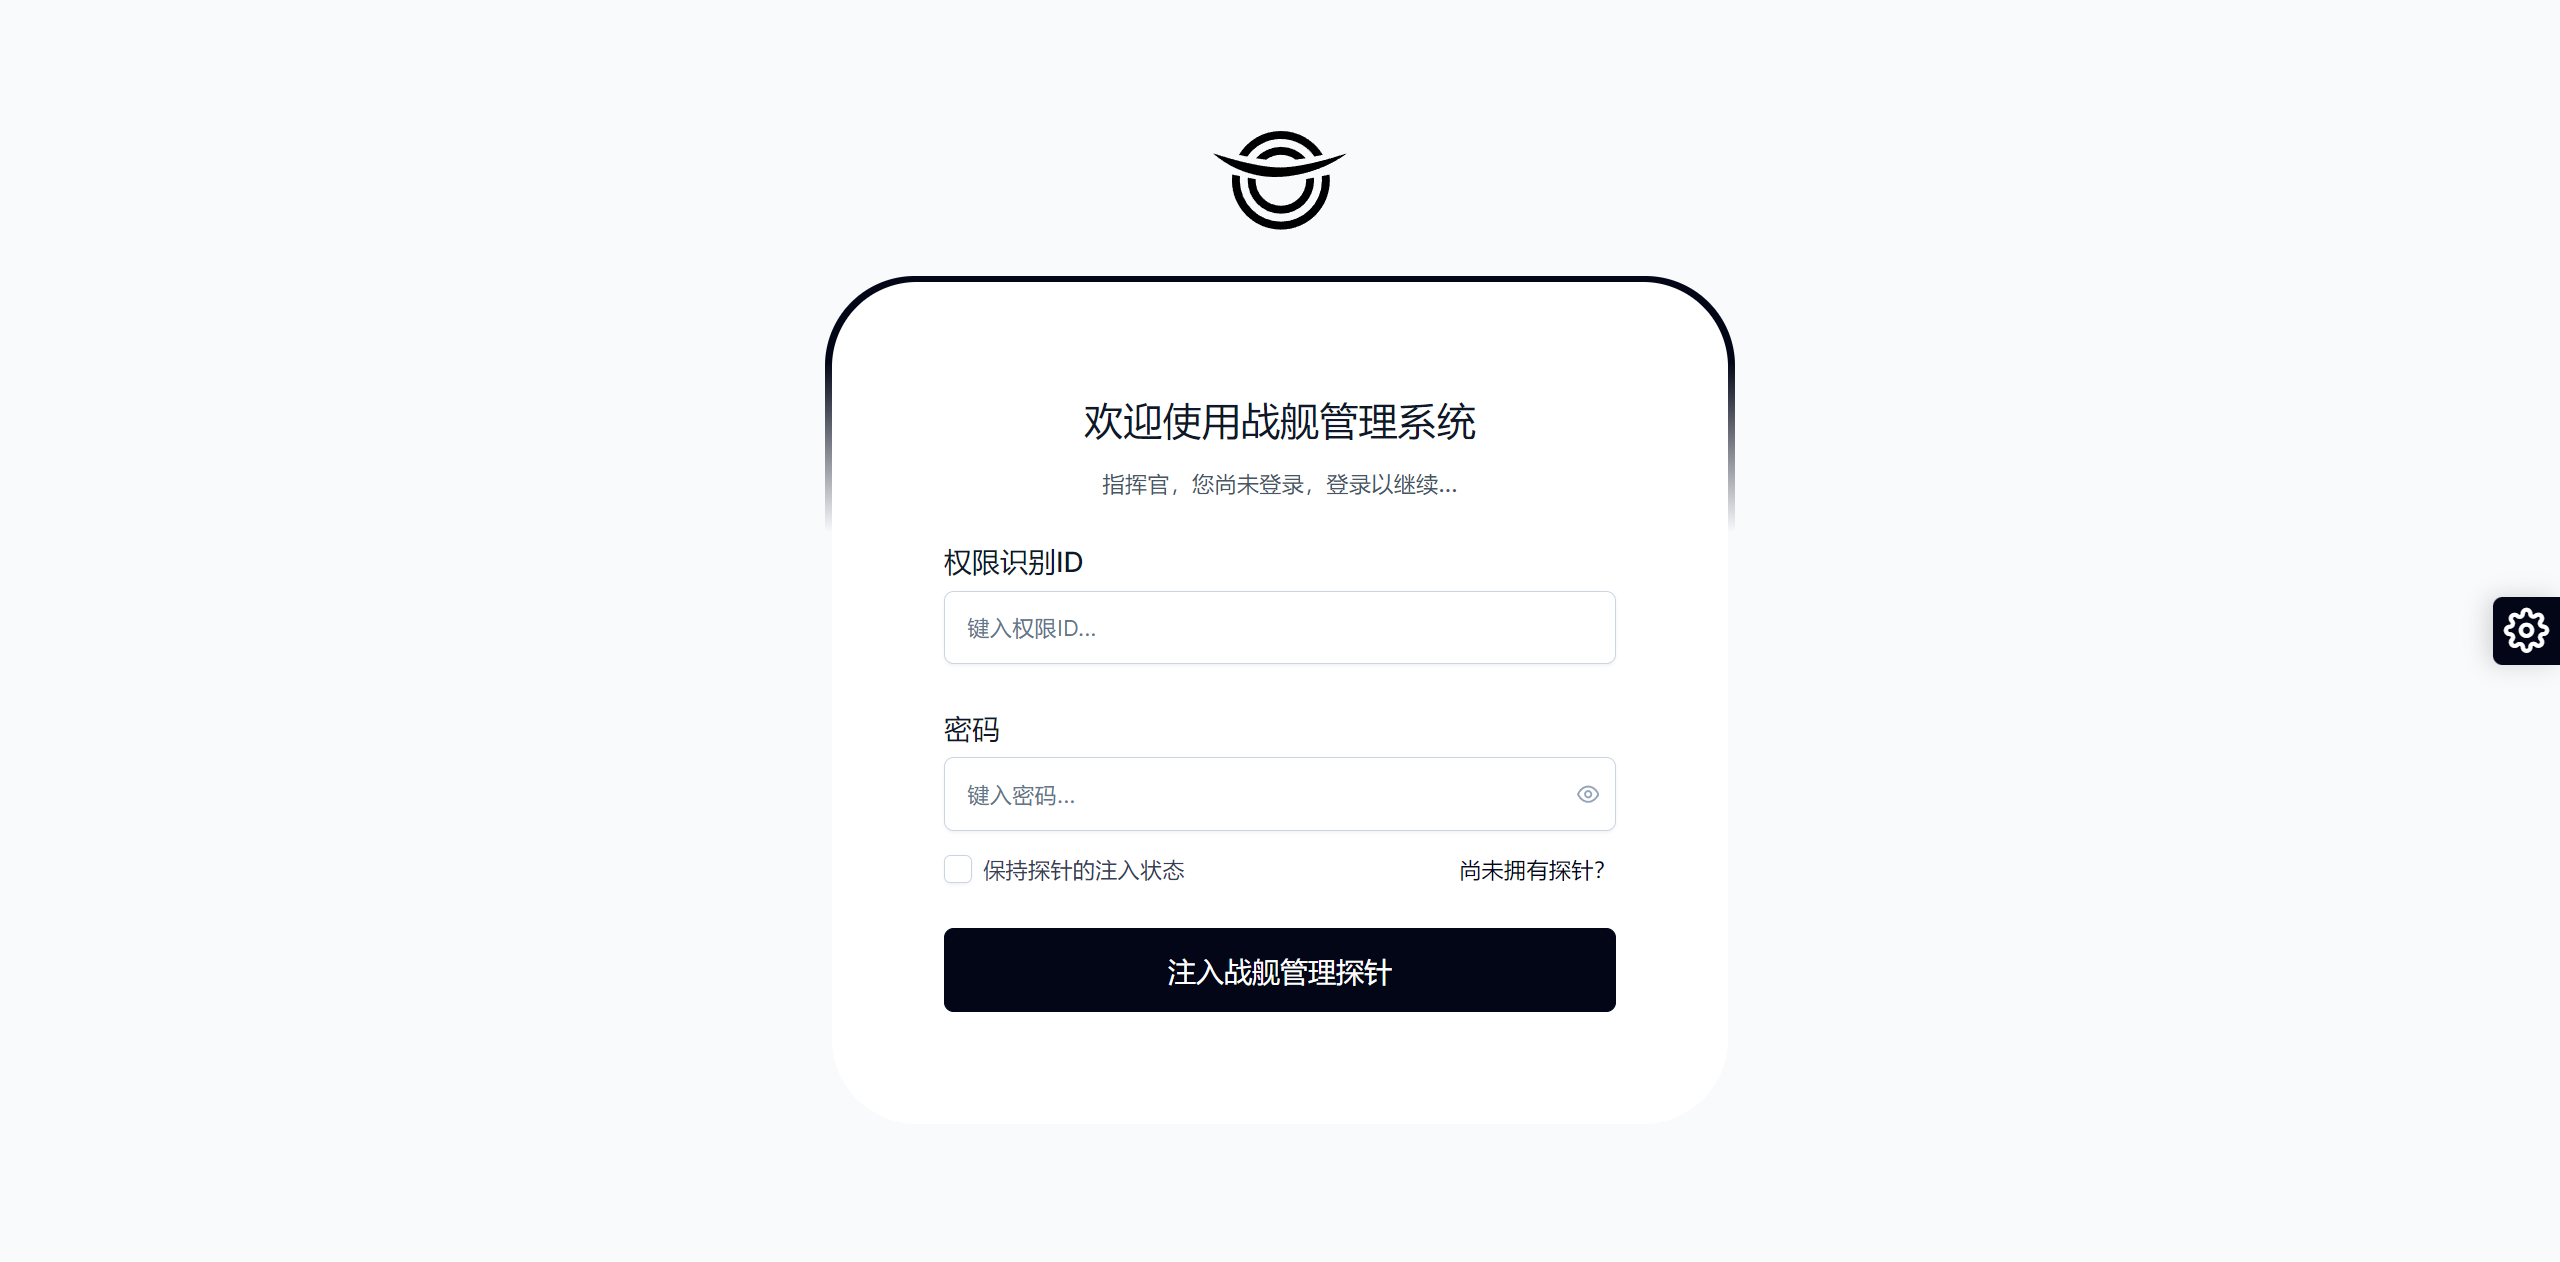
\includegraphics[width=\linewidth]{images/LoginPage}
	\caption{登录界面}
	\label{fig:loginpage}
\end{figure}

为了使得项目更加有趣味和带有科幻色彩,登录账号、登录密码等描述,均被替换为一些看起来“略显科幻”的词句。

由于使用了 PrimeVue 主题的套件,登录界面只需引入组件即可完成构建。后面的界面均是由 PrimeVue 的组件构成,不再赘述其排布方式,因其可以很容易从图中观察到。

用户输入错误的账号或密码时,会直接弹出该提示:

% TODO: \usepackage{graphicx} required
\begin{figure}[H]
	\centering
	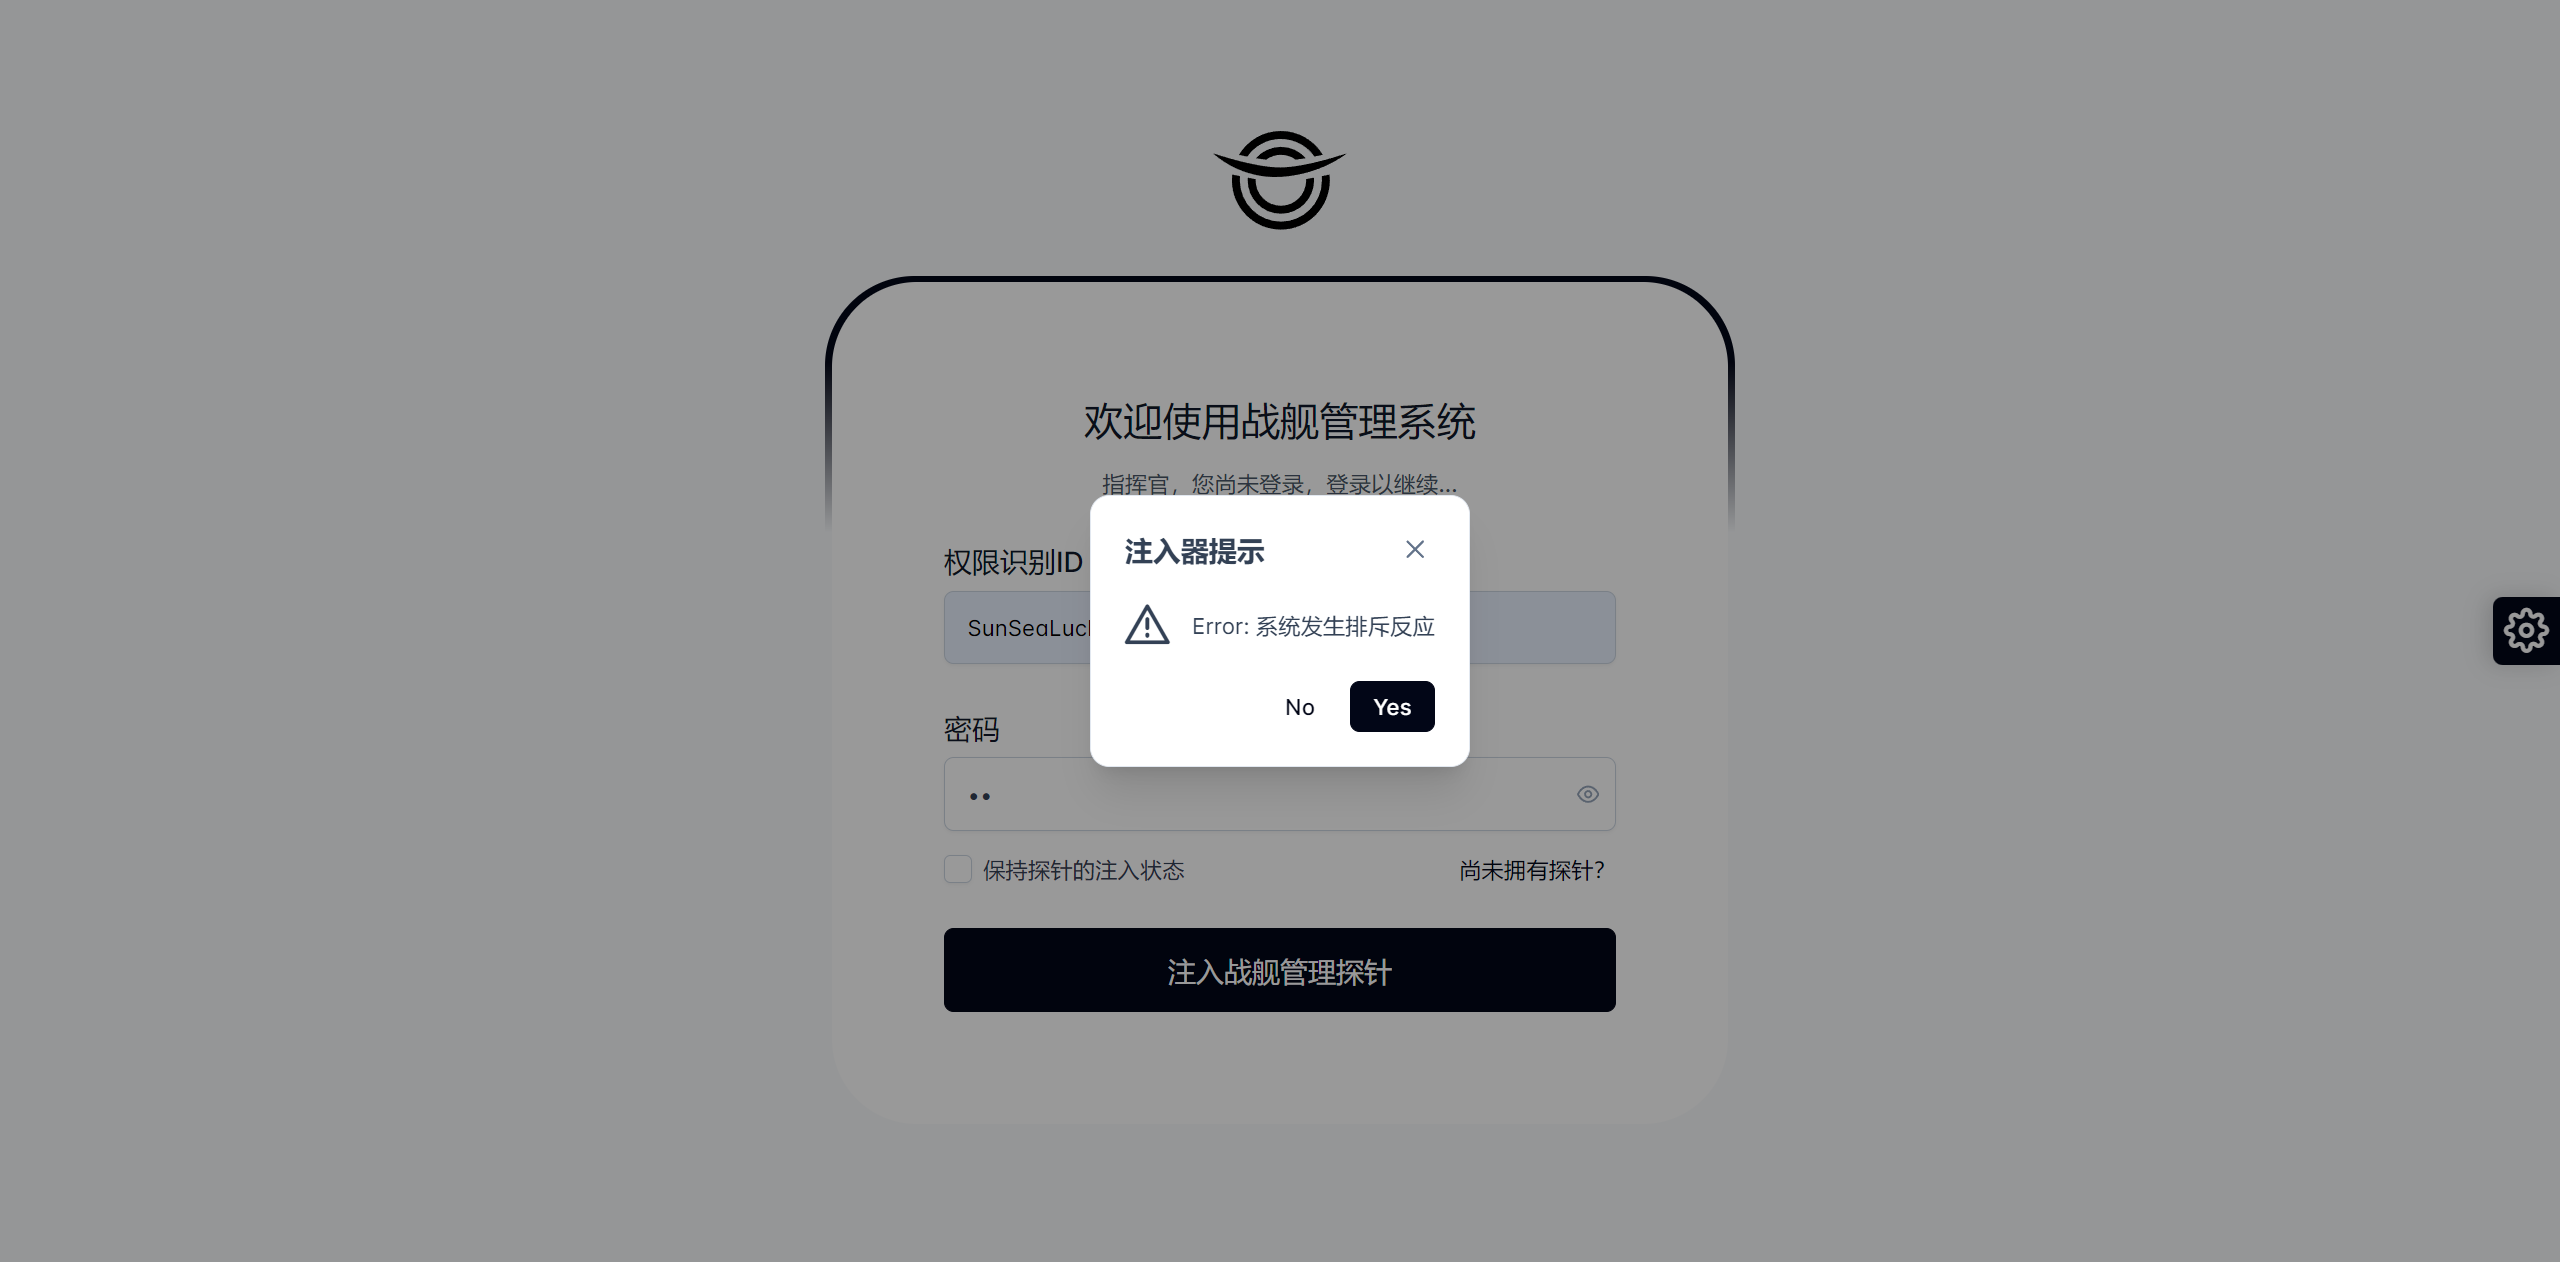
\includegraphics[width=\linewidth]{images/ErrorMsgBox}
	\caption{错误弹窗提示}
	\label{fig:errormsgbox}
\end{figure}

用户登录界面需要访问 /auth/register 路径,也可以通过点击登录界面的“尚未拥有探针”提示来进入注册界面。

% TODO: \usepackage{graphicx} required
\begin{figure}[H]
	\centering
	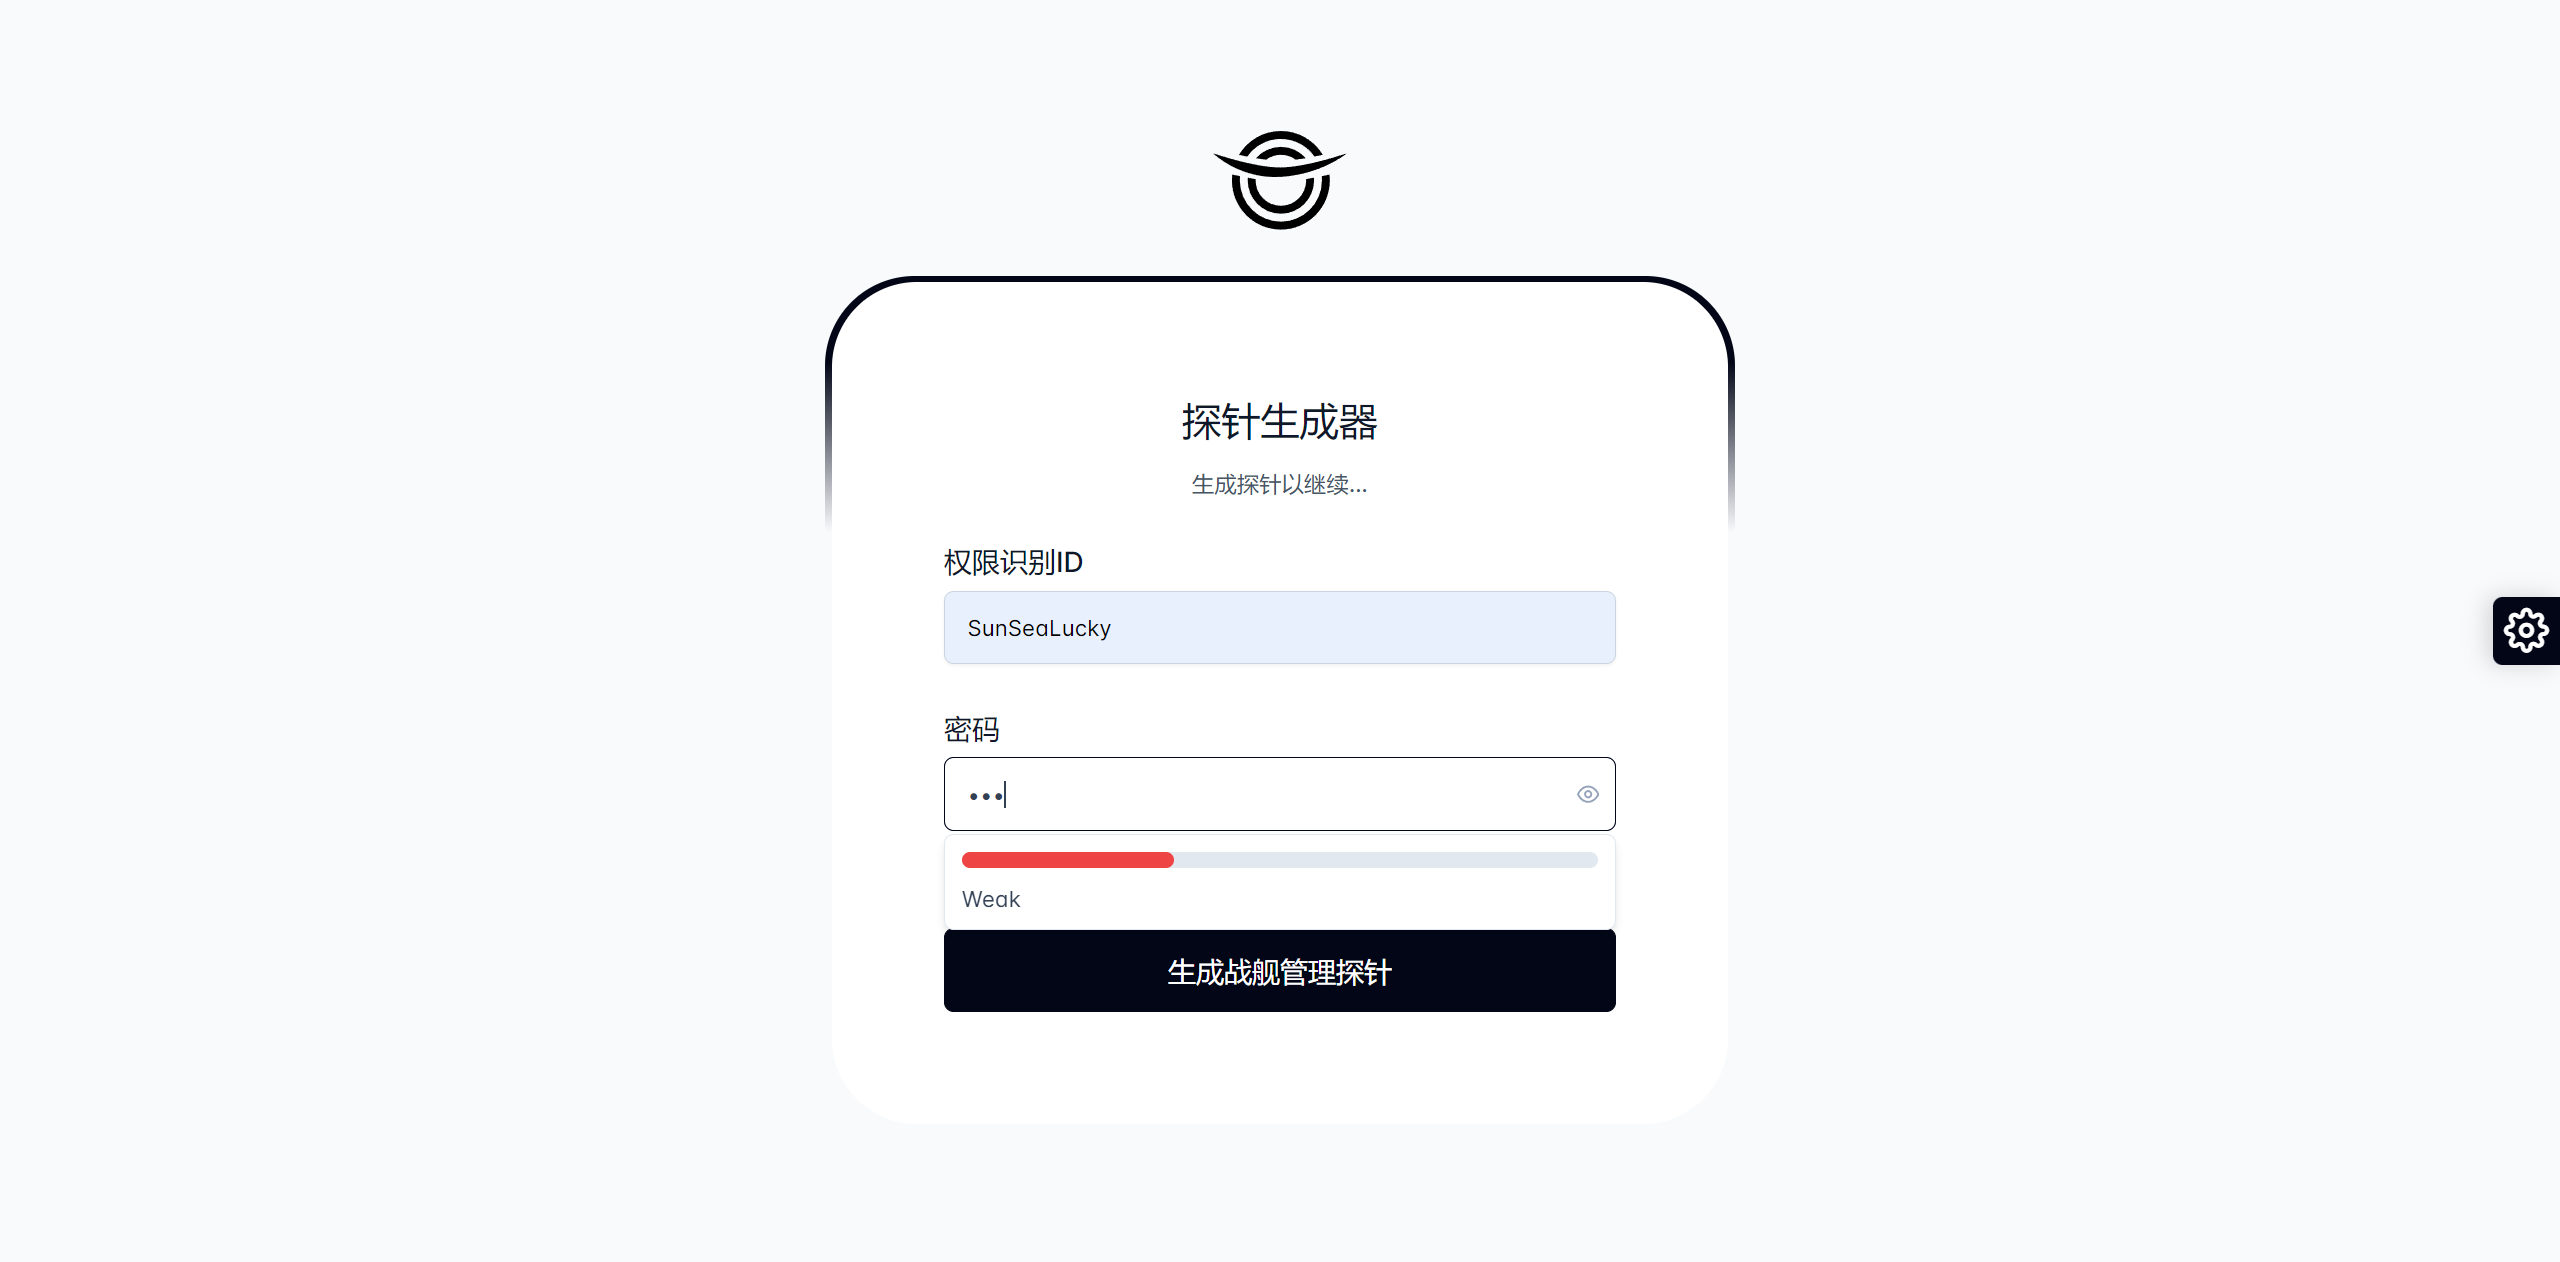
\includegraphics[width=\linewidth]{images/RegisterPage}
	\caption{注册界面(密码带有强弱等级提示)}
	\label{fig:registerpage}
\end{figure}

注册后,返回到登陆界面登录,可看到右上角的绿色的登录成功提示:

% TODO: \usepackage{graphicx} required
\begin{figure}[H]
	\centering
	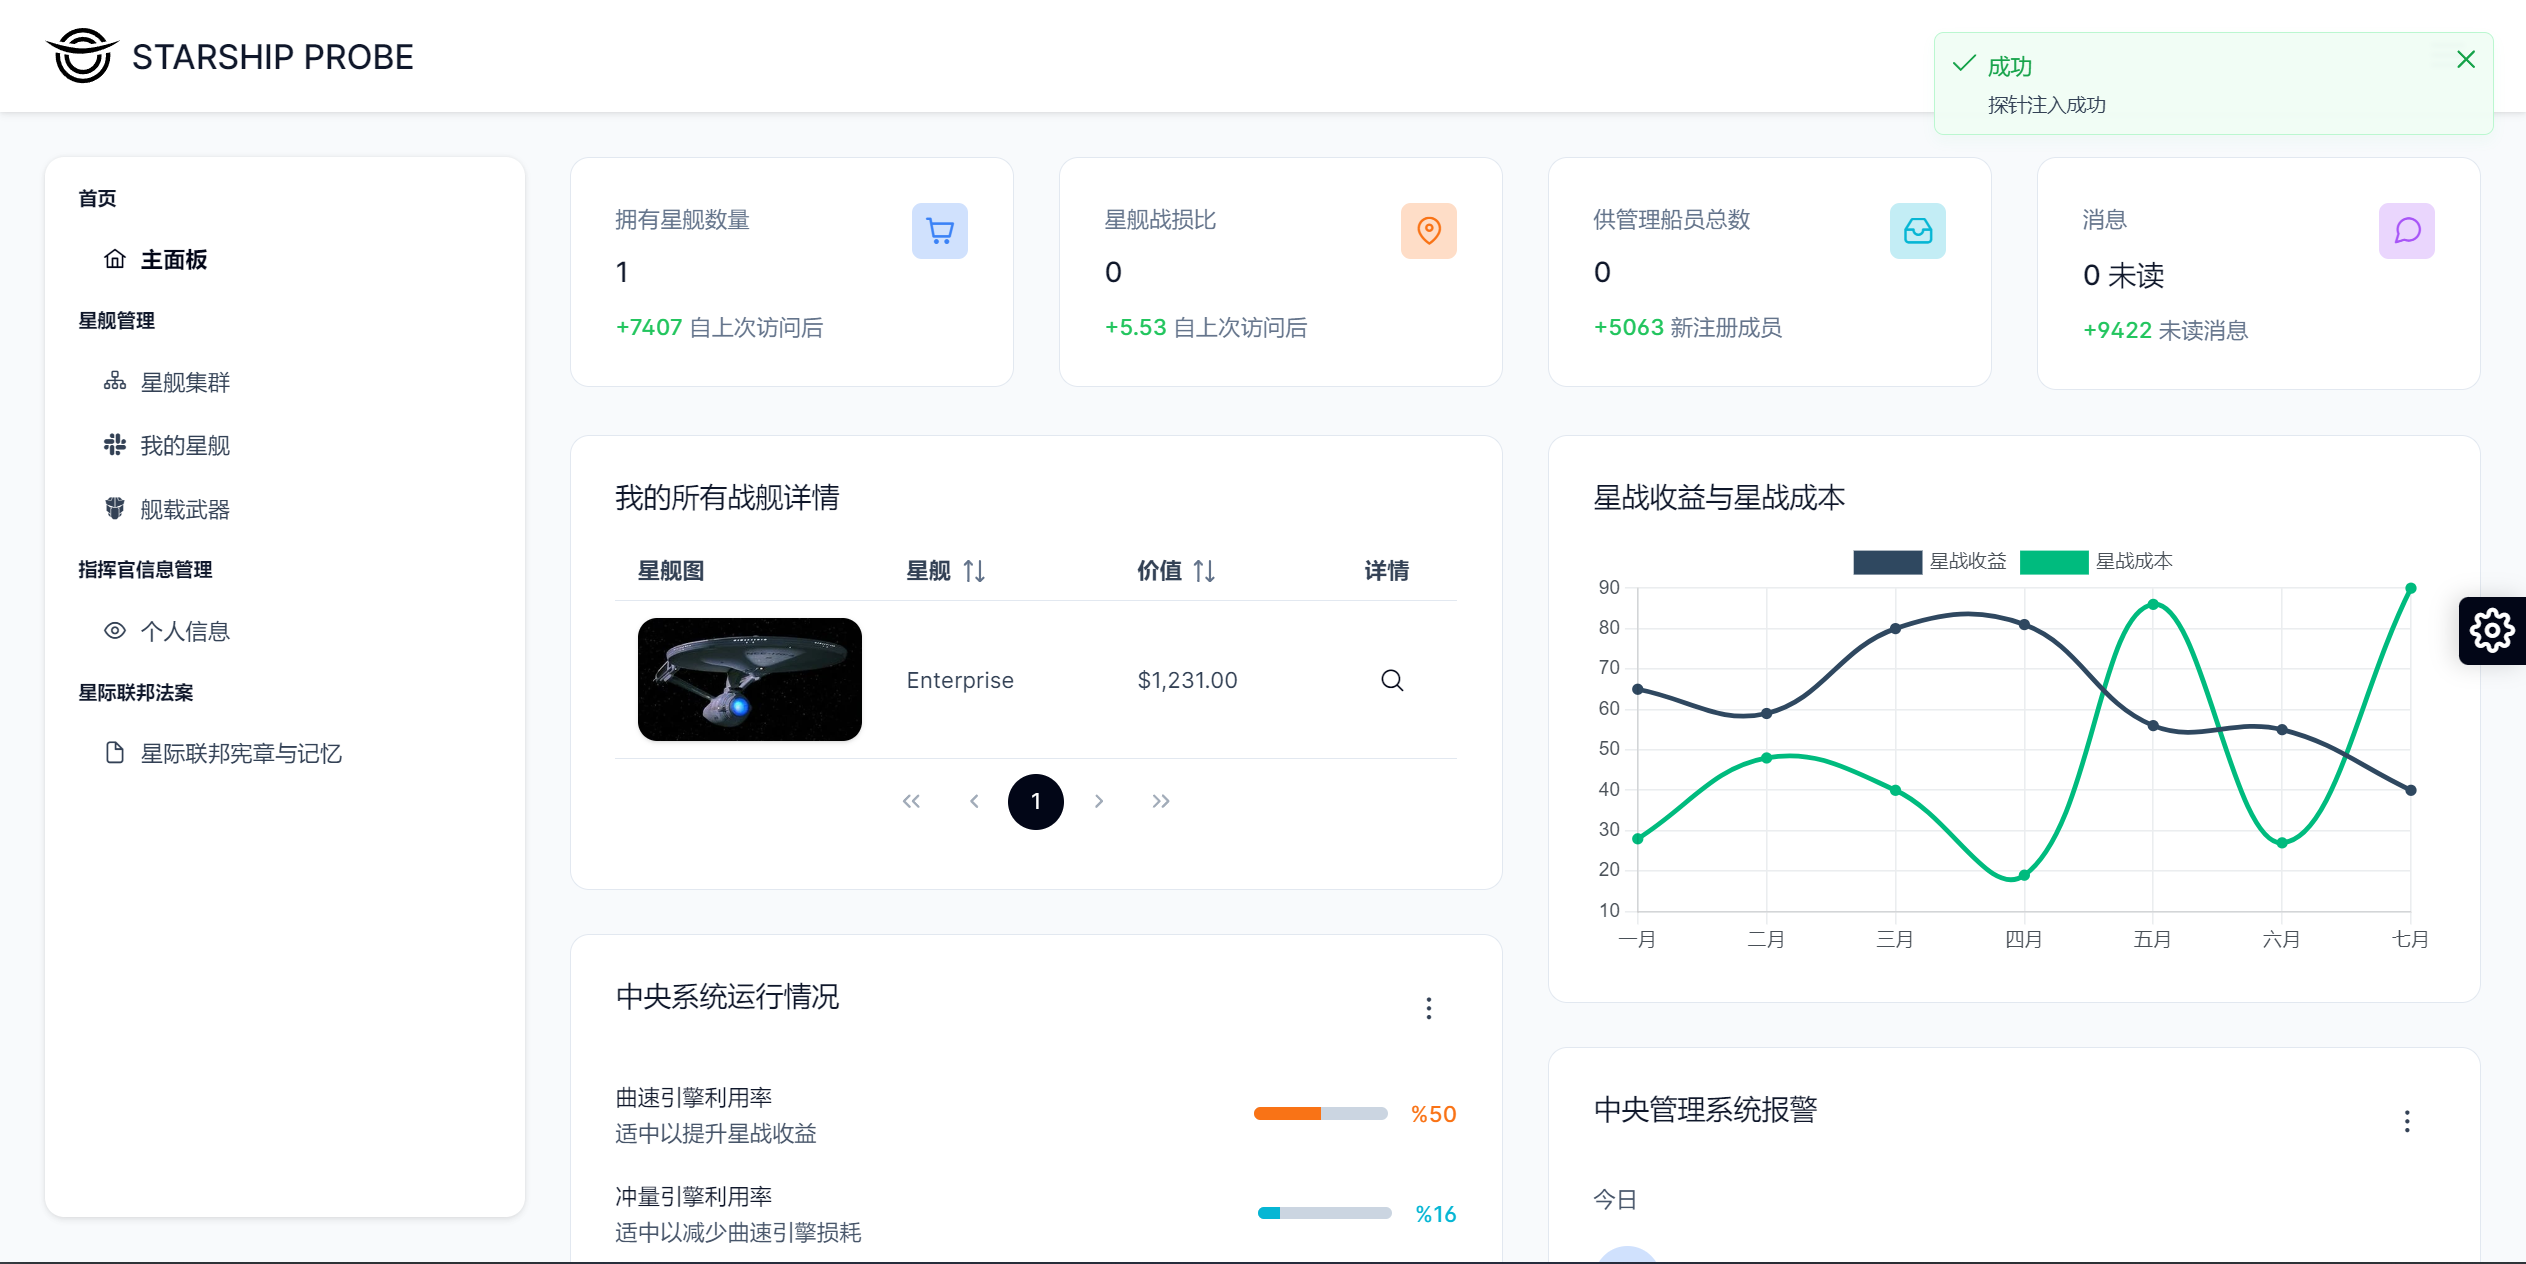
\includegraphics[width=\linewidth]{images/LoginSuccess}
	\caption{登录成功进入主面板}
	\label{fig:loginsuccess}
\end{figure}

用户状态的持久化存储使用 Pinia 和 JWT,上面已经介绍过,不再赘述:

\begin{verbatim}
	import { defineStore } from 'pinia';
	import { ref } from 'vue';
	
	export const useTokenStore = defineStore(
	'token',
	() => {
		const token = ref('');
		
		const setToken = newToken => {
			token.value = newToken;
		};
		const removeToken = () => {
			setToken('');
		};
		return {
			token, setToken, removeToken
		};
	},
	{
		persist: true
	}
	);
	
\end{verbatim}

\subsubsection{主面板的设计}

% TODO: \usepackage{graphicx} required
\begin{figure}[H]
	\centering
	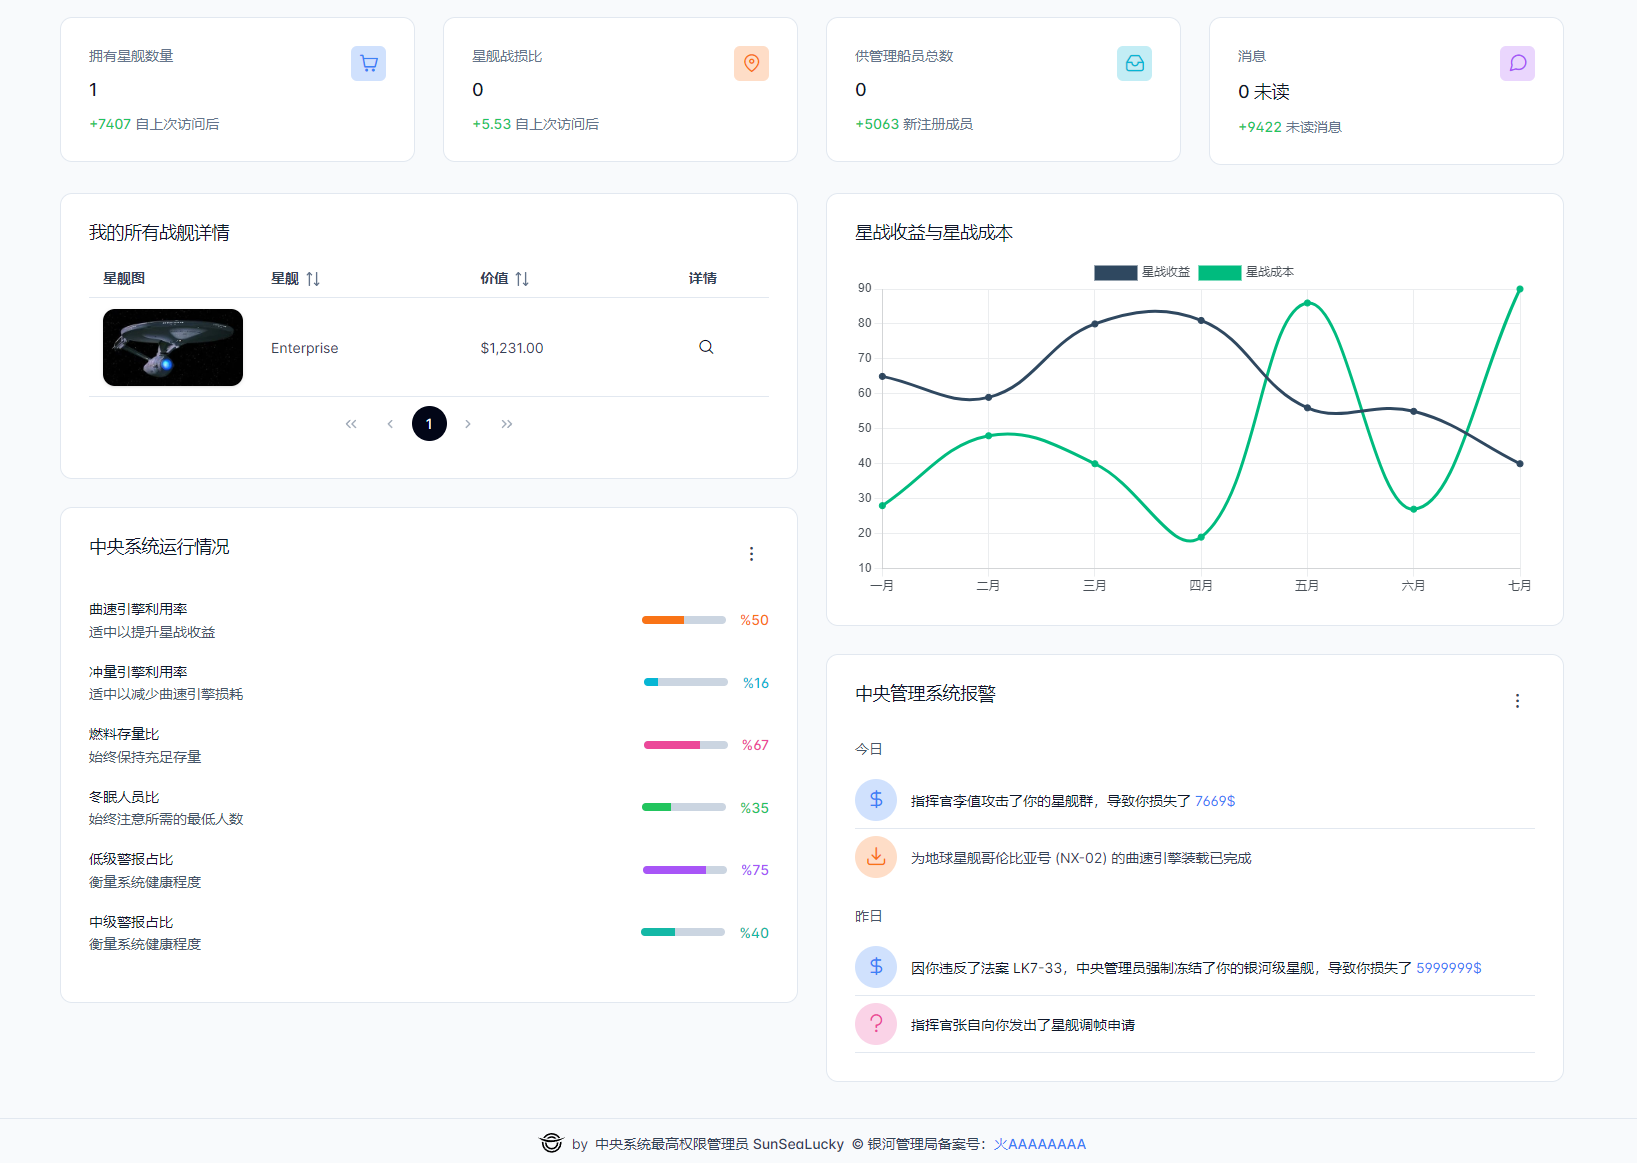
\includegraphics[width=\linewidth]{images/Dashboard}
	\caption{主面板内容}
	\label{fig:dashboard}
\end{figure}

界面上方提供了几个关键指标的概览,拥有星舰数量(当前玩家拥有一艘星舰,自上次访问后增加了7407艘)、星舰战损比、供管理船员总数、消息。

中间部分显示了“我的所有战舰详情”,其中列出了玩家的星舰数量、价值等简要信息。下方有一个图表,显示了中央系统运行的情况,包括曲速引擎利用率、冲量引擎利用率、燃料存量比、冬眠人员比、低级警报占比和中级警报占比。

右侧是一个关于“星战收益与星战成本”的折线图,可以对比这两项指标随时间的变化趋势。下面还有一个“中央管理系统报警”列表,记录了最近发生的事件,包括指挥官的攻击导致的损失以及完成的维护任务。

底部注明了该界面由“中央系统最高权限管理员 SunSeaLucky”提供,并附带了一个银河管理局备案号,此为仿照真实世界网站,仅供装饰之用。

\subsubsection{侧边栏设计}
侧边栏分为三个部分,第一个部分是主面板。第二个部分是星舰集群、我的星舰、舰载武器,第三个部分是指挥官信息管理,第四个部分是星际联邦宪章与记忆。

\textbf{主面板}查看星舰探测器的实时数据和统计信息;\textbf{星舰集群}查看和管理多个星舰的集群;\textbf{我的星舰}查看和编辑个人星舰的详细信息;\textbf{舰载武器}管理星舰装备;\textbf{个人信息}编辑个人资料和偏好设置;\textbf{星际联邦宪章与记忆}获取历史记录和法规知识。

\subsubsection{星舰的管理与购买}

该页面的用于查看星舰的表格有十个特性。\textbf{筛选条件},用户可以通过输入关键词搜索星舰,也可以清除已有的筛选条件;\textbf{星舰图片},展示每艘星舰的图像,方便识别;\textbf{星舰代号},星舰的唯一标识符;\textbf{生产国家},制造星舰的国家;当前运行代理,当前负责运营星舰的角色;\textbf{生产日期},星舰制造的时间;\textbf{当前估值},星舰当前的市场价值;\textbf{舰体状态},显示星舰的状态,如“即将报废”;\textbf{运行负载},显示星舰的负载情况;\textbf{星舰验证},显示星舰是否通过验证,用绿色勾选标记表示已验证。

% TODO: \usepackage{graphicx} required
\begin{figure}[H]
	\centering
	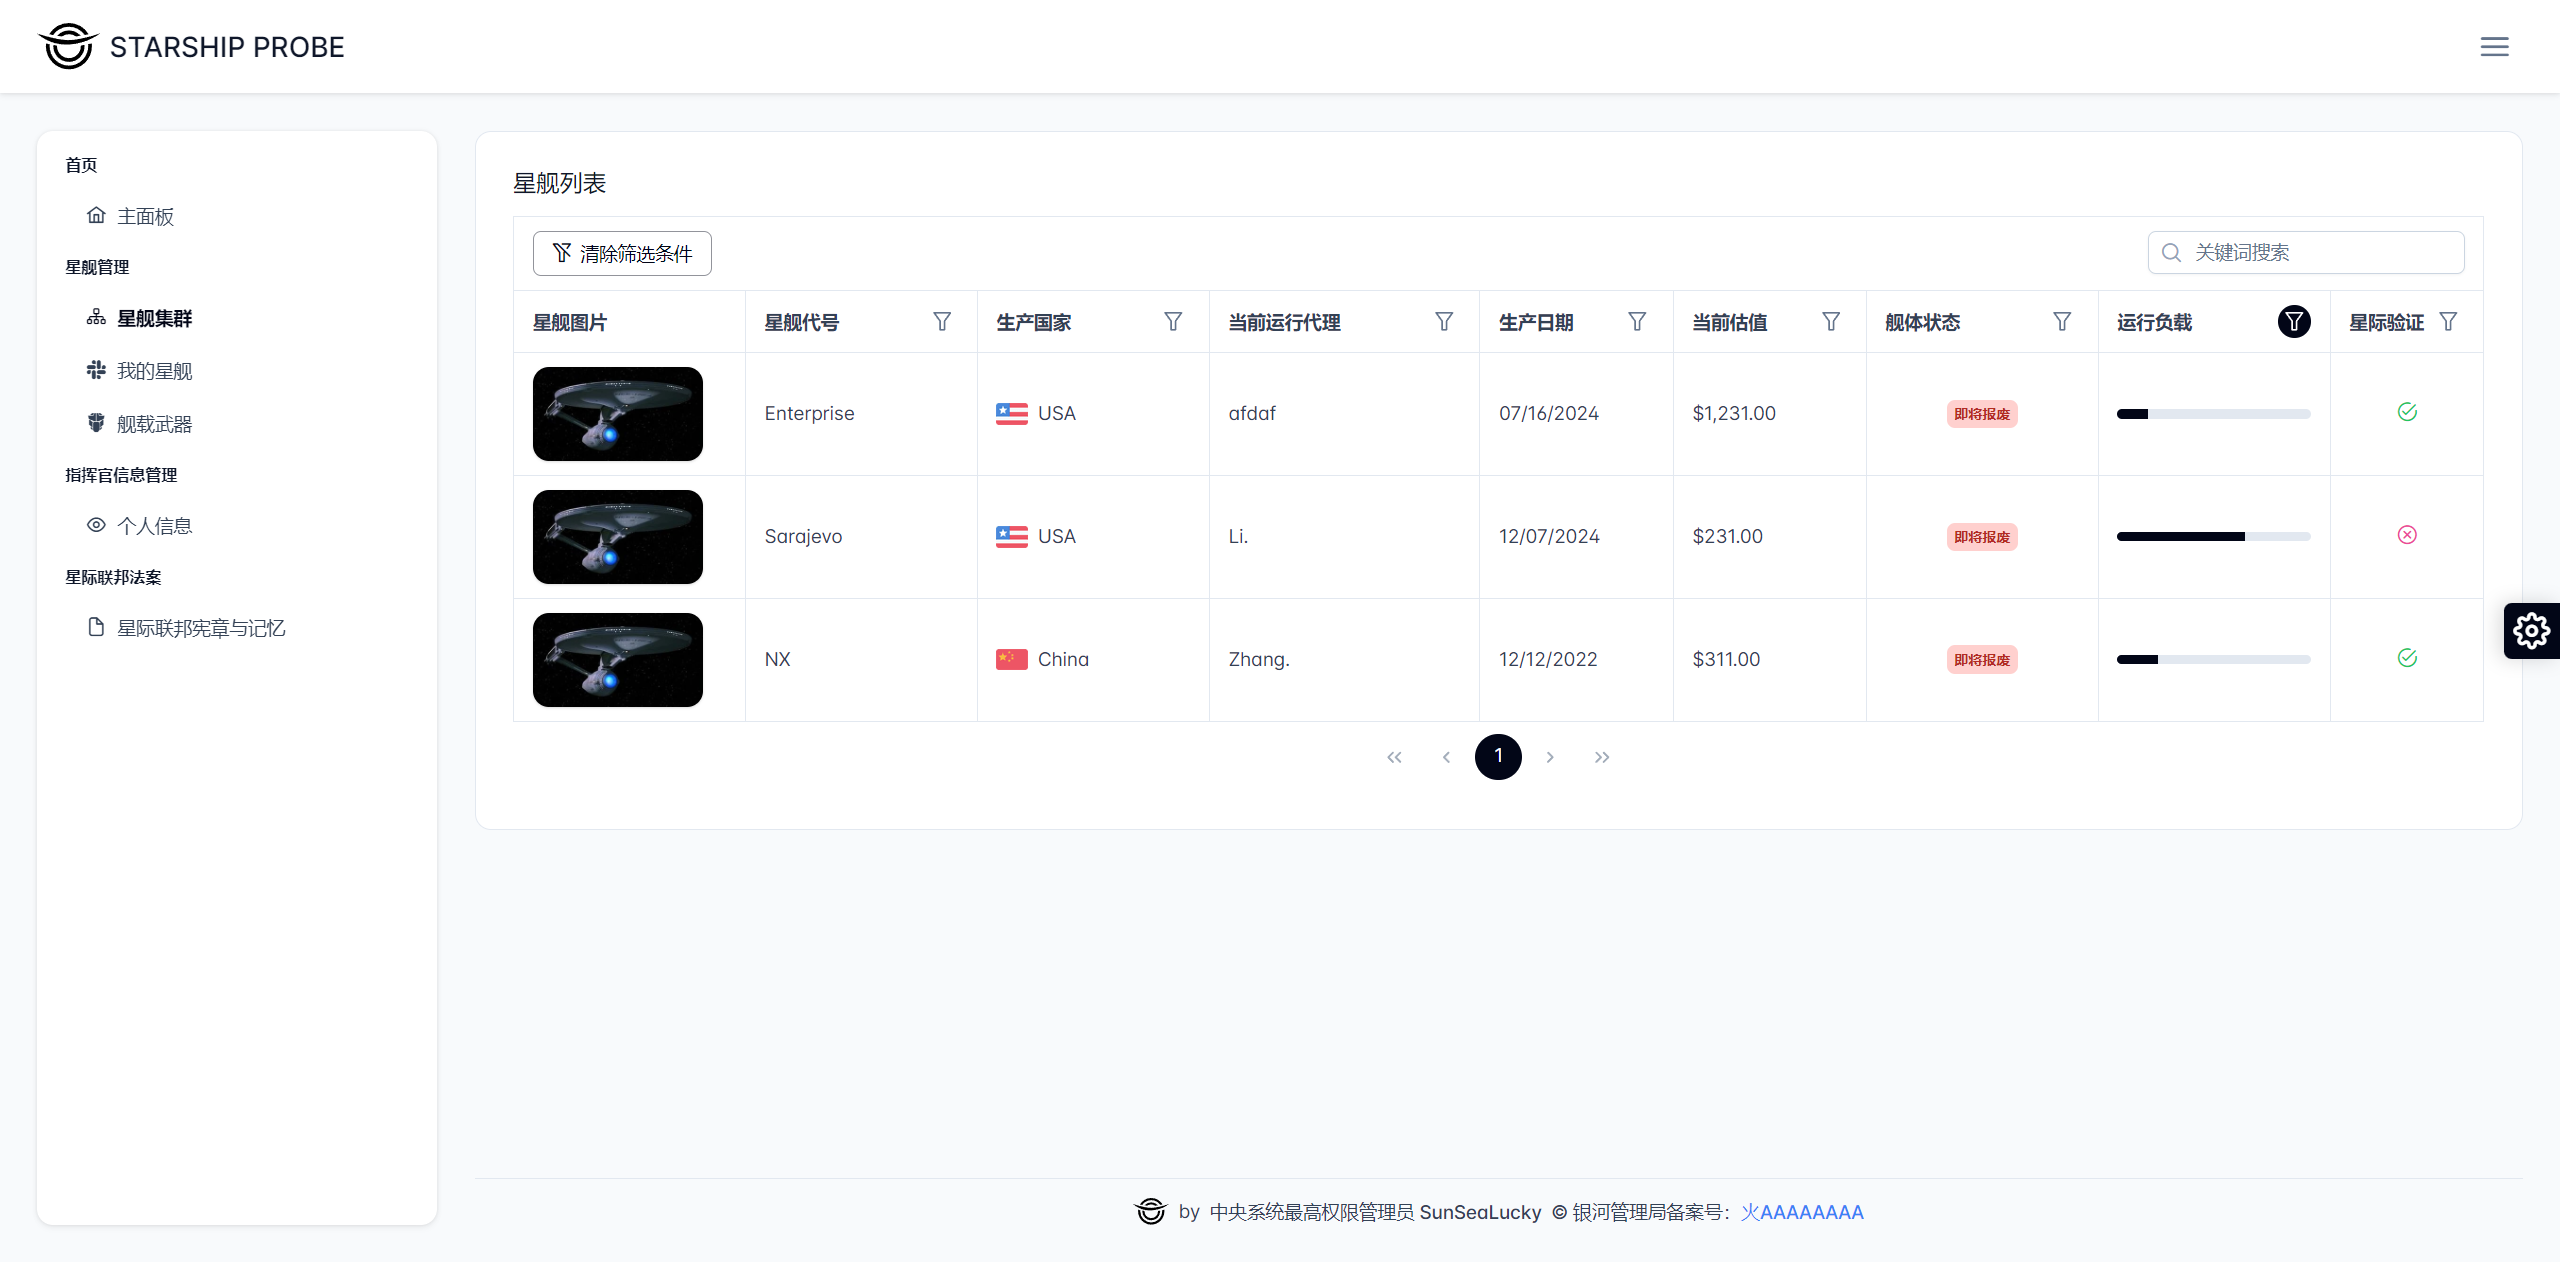
\includegraphics[width=\linewidth]{images/StarshipMarket}
	\caption{星舰市场页}
	\label{fig:starshipmarket}
\end{figure}

此页面不可直接增删改,因为该页面代表的是市场正在出售的星舰。若需购买星舰,需要先复制好自己想要购买的星舰的代号,然后跳转至“我的星舰”页面。

星舰的购买与售出,可见图 \ref{fig:mystatshippage} 至图 \ref{fig:salestarship} 。

\textbf{我的星舰}页主要展示用户拥有的星舰信息并提供相关操作。页面包含以下元素:
\begin{enumerate}
	\item 当前余额 - 显示用户的可用资金,用于购买或维护星舰。
	\item 顶部侧有三个按钮
	\begin{itemize}
		\item 购买星舰,允许用户使用当前余额购买新的星舰。
		\item 卖出星舰,用户可以出售已拥有的星舰以回收资金。
		\item 导出星舰数据,可将星舰信息导出,方便备份或分析。
	\end{itemize}
	
	\item 表格,列出了用户目前拥有的星舰详情:
	\item 当前代理 ,星舰当前的负责人或运营商。
	\item 星舰,星舰的名字,例如 "Enterprise"。
	\item 星舰图片,星舰的图标或标志。
	\item 当前估值,星舰的当前市场价值,例如 "\$1,231.00"。
	\item 所属类别,星舰的分类编号,这里是 "16"。
	\item 生产国家,星舰的制造国家,比如 "USA"。
	\item 星舰状态,显示星舰的状态。
	\item 操作列,包含两个操作按钮。绿色的 "编辑" 按钮允许用户修改星舰的信息;红色的 "删除" 按钮可删除所选星舰。
	\item 分页,页面底部显示了分页控件,让用户可以在多页星舰之间切换,当前显示第1页,共1艘星舰,每页最多显示10艘星舰。
	\item 搜索框,在表格上方有一个搜索框(Search...),用户可以在此输入关键词来过滤星舰列表。

\end{enumerate}



% TODO: \usepackage{graphicx} required
\begin{figure}[H]
	\centering
	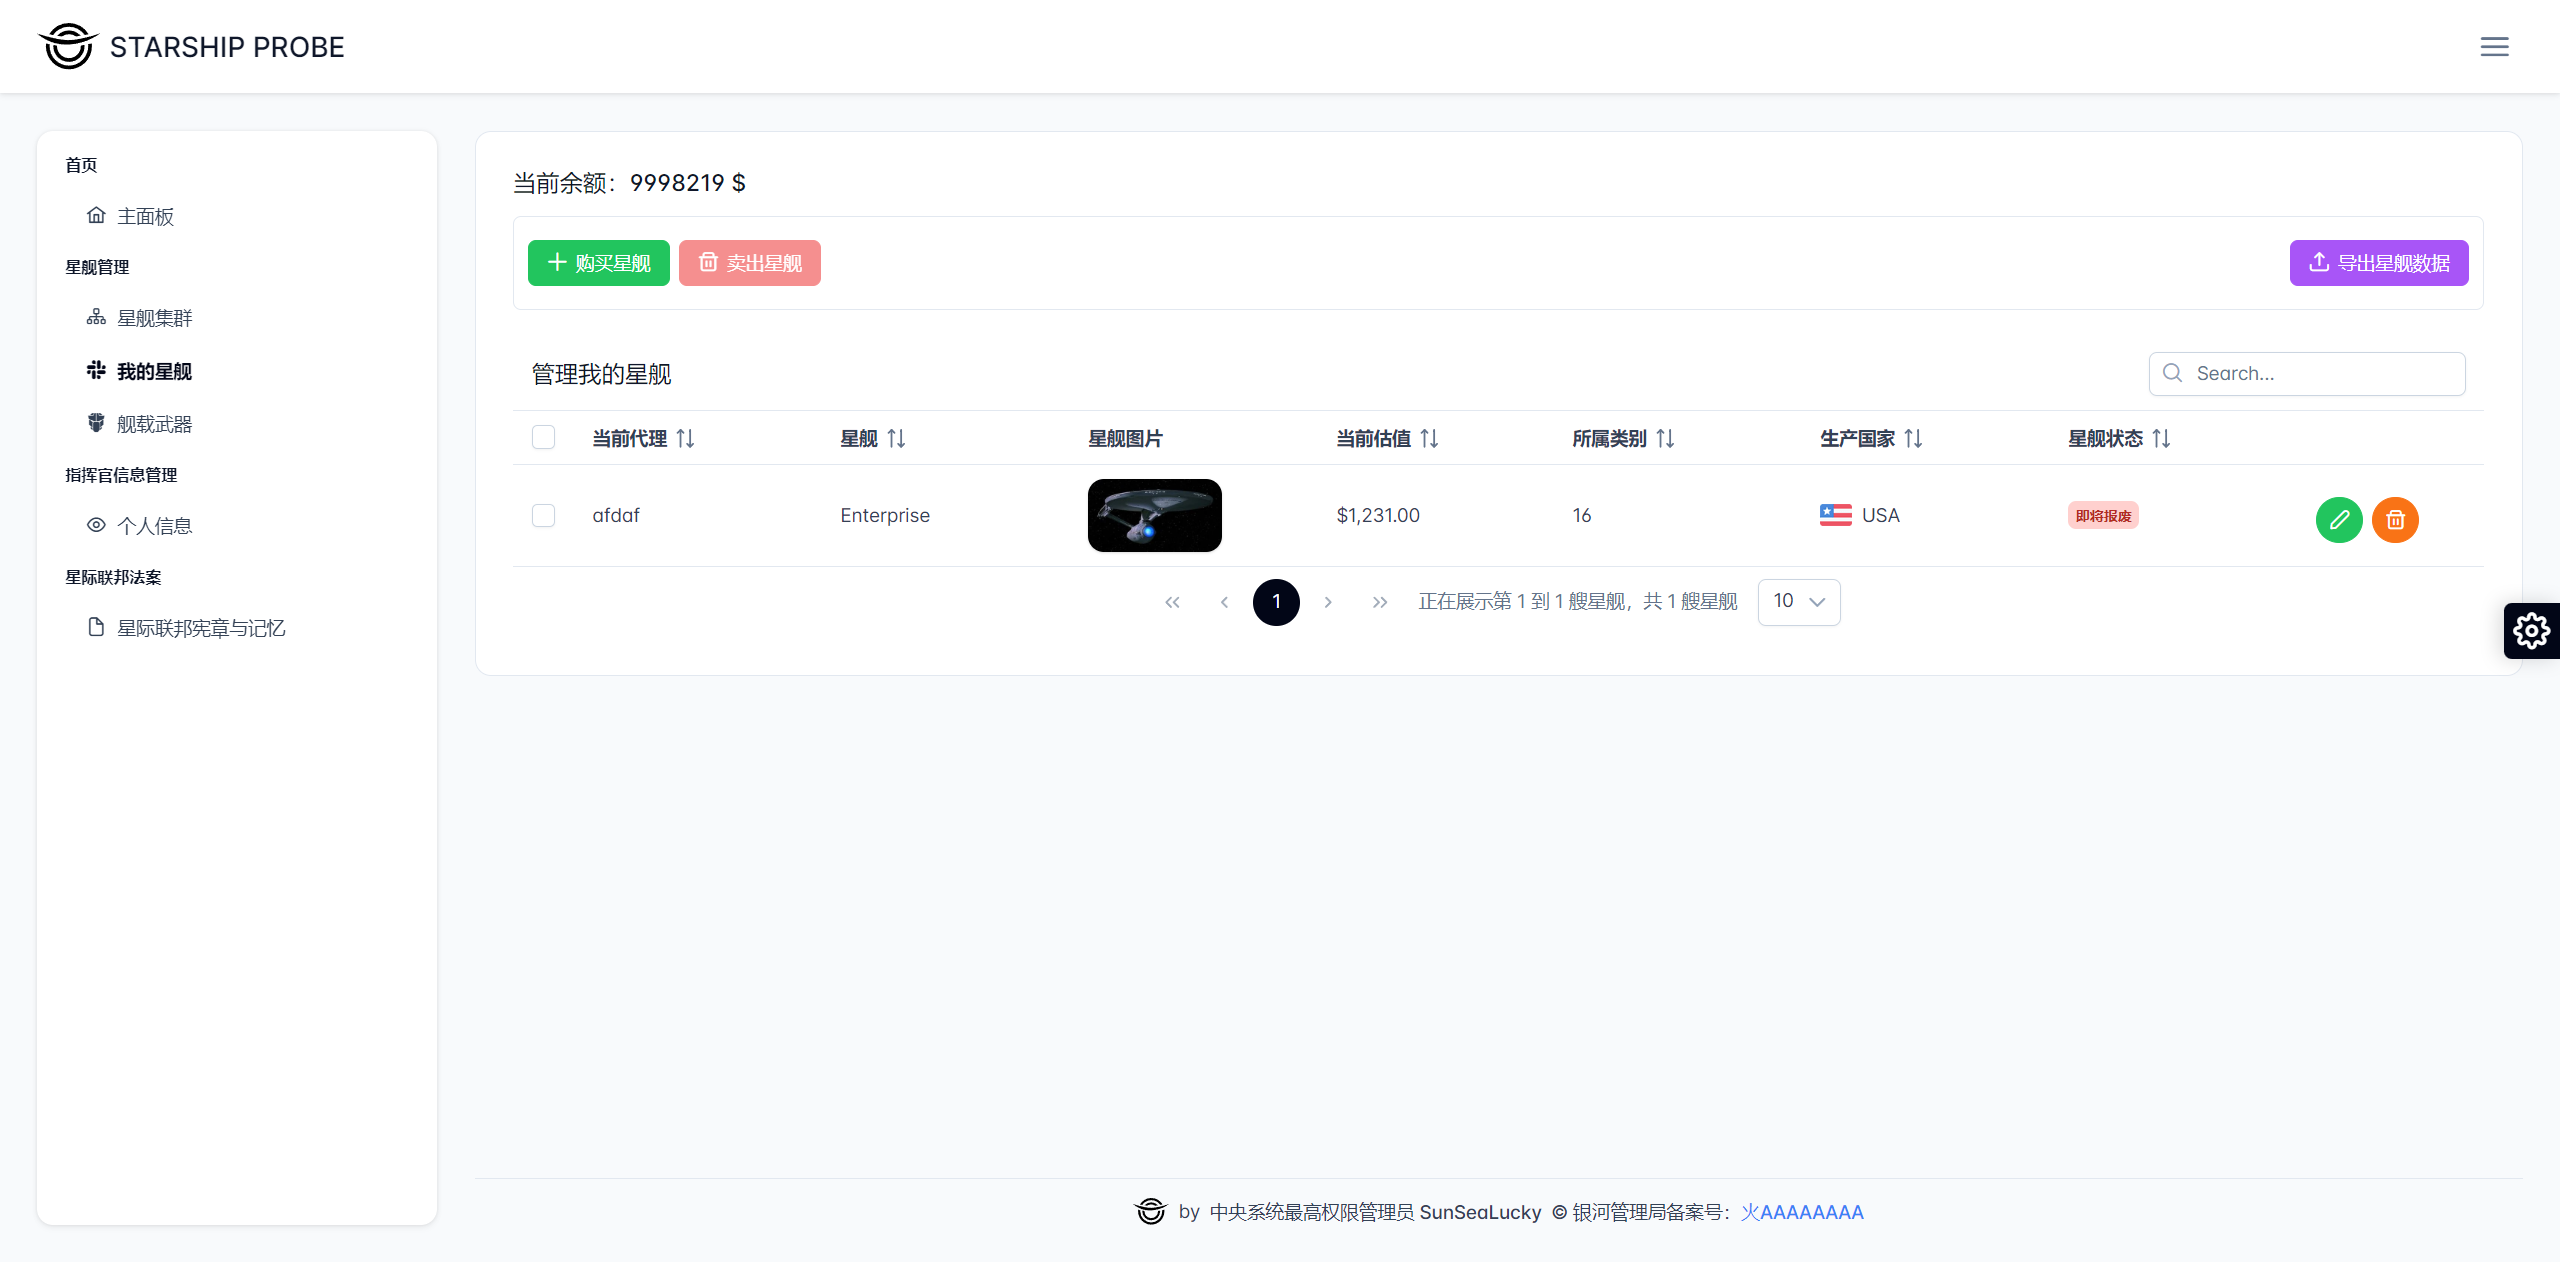
\includegraphics[width=\linewidth]{images/MyStatshipPage}
	\caption{我的星舰页}
	\label{fig:mystatshippage}
\end{figure}

% TODO: \usepackage{graphicx} required
\begin{figure}[H]
	\centering
	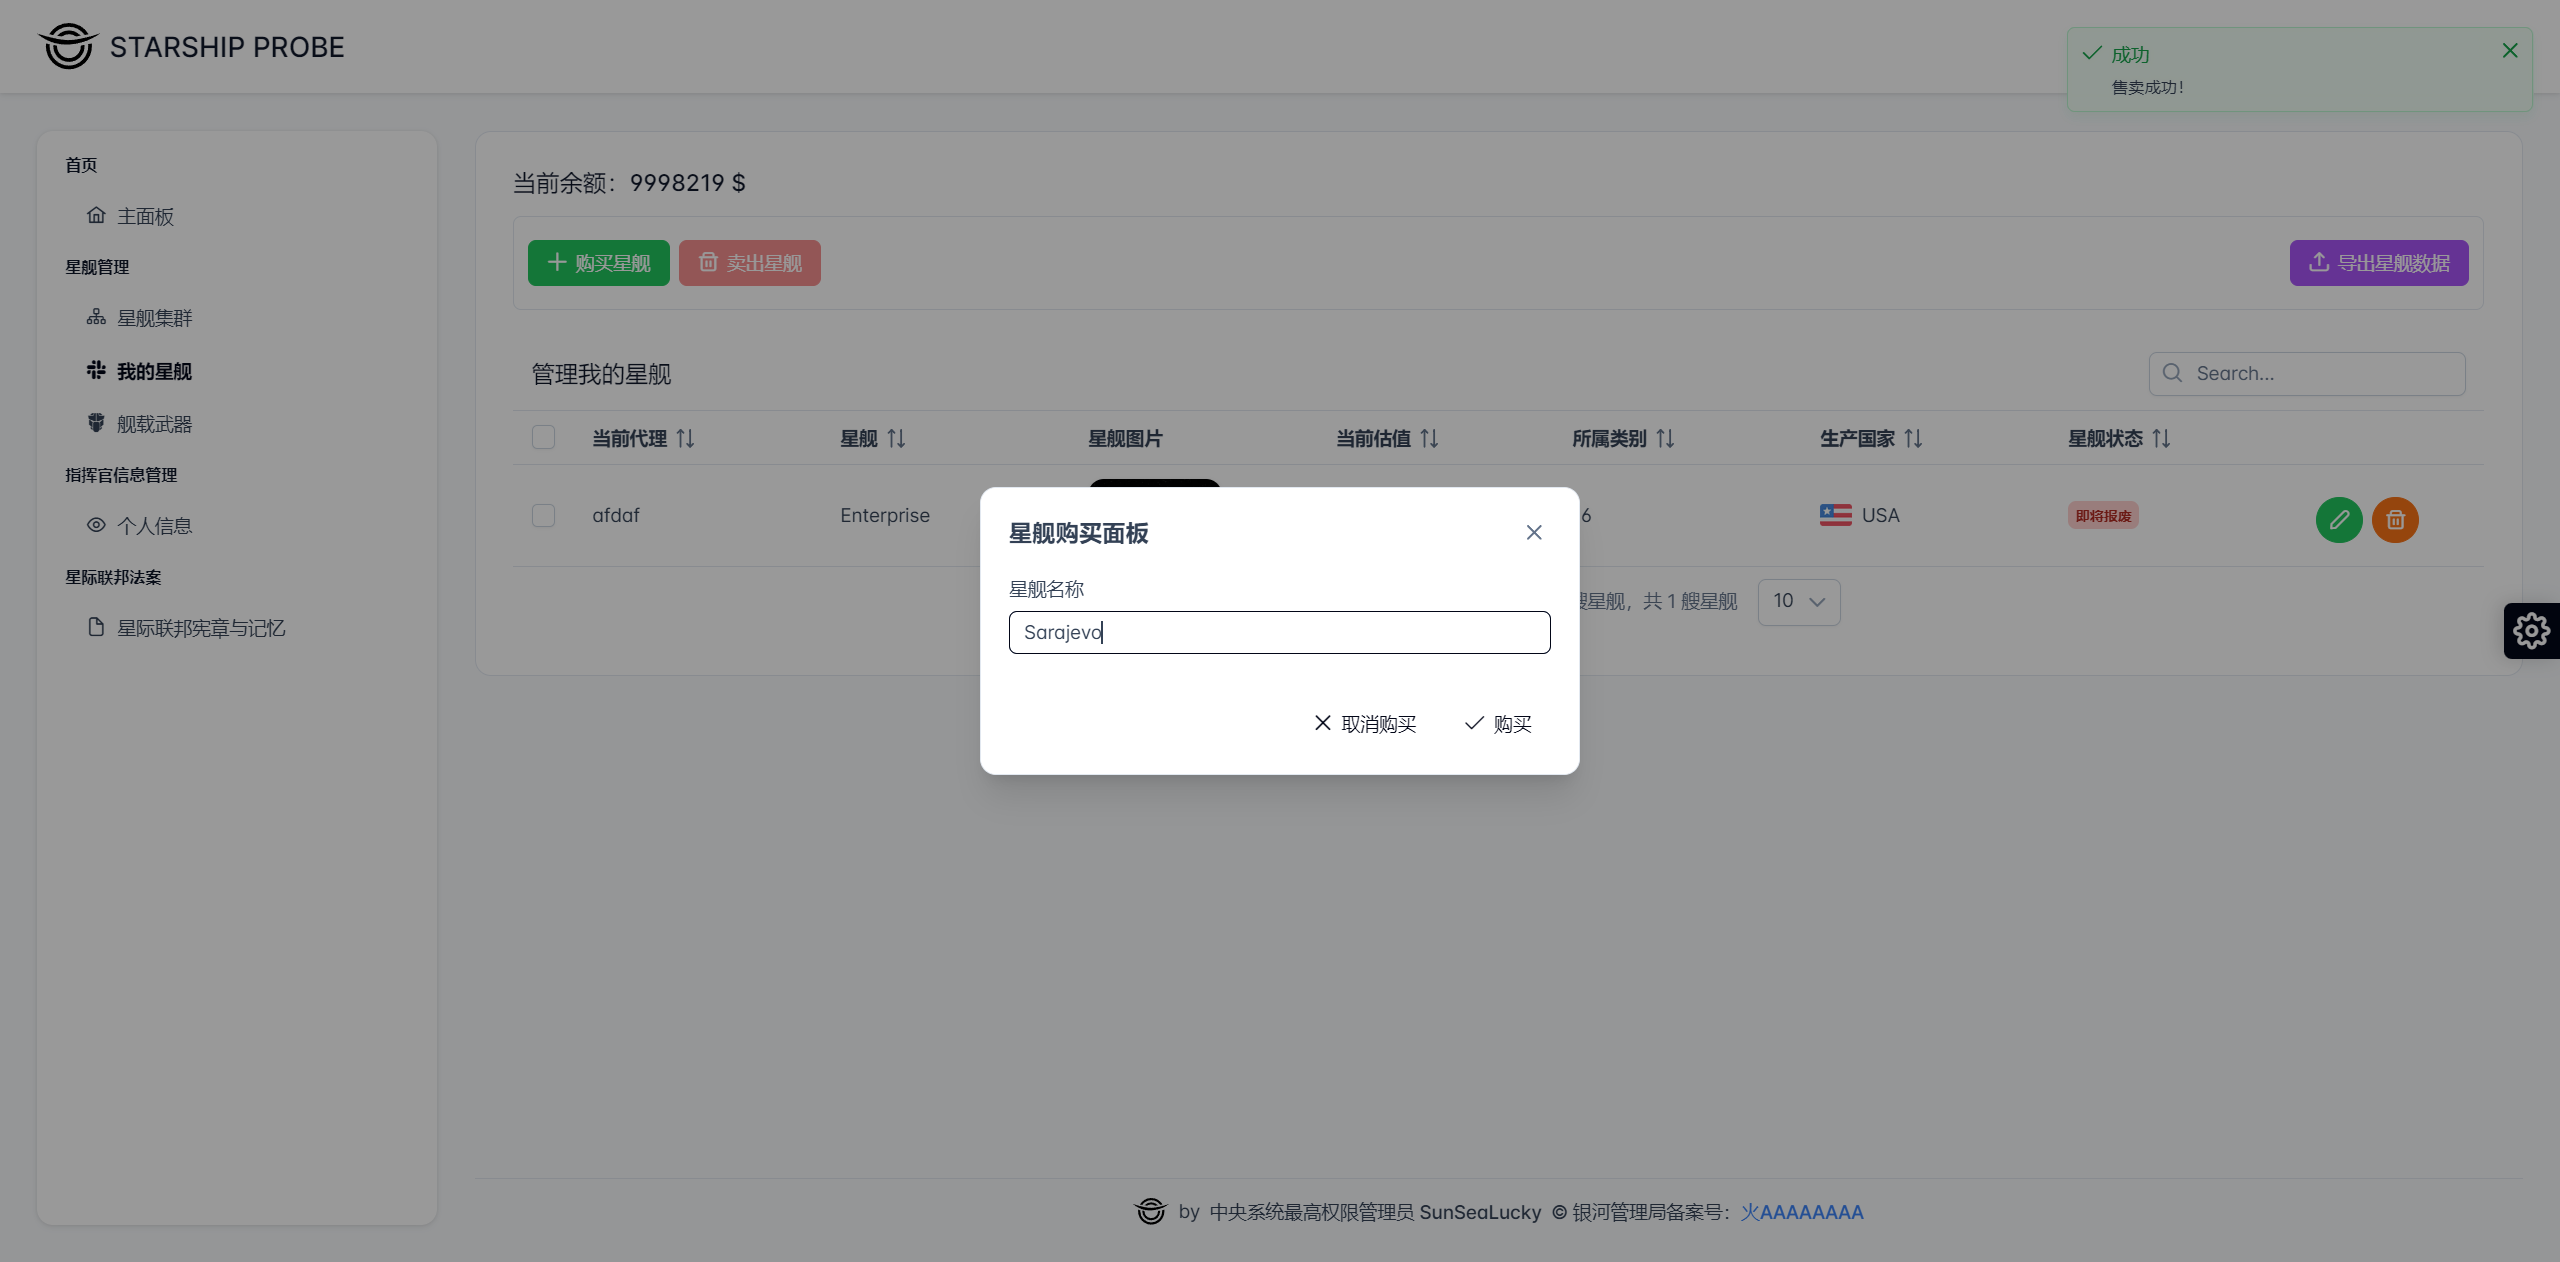
\includegraphics[width=\linewidth]{images/BuyStarship}
	\caption{购买星舰页}
	\label{fig:buystarship}
\end{figure}


% TODO: \usepackage{graphicx} required
\begin{figure}[H]
	\centering
	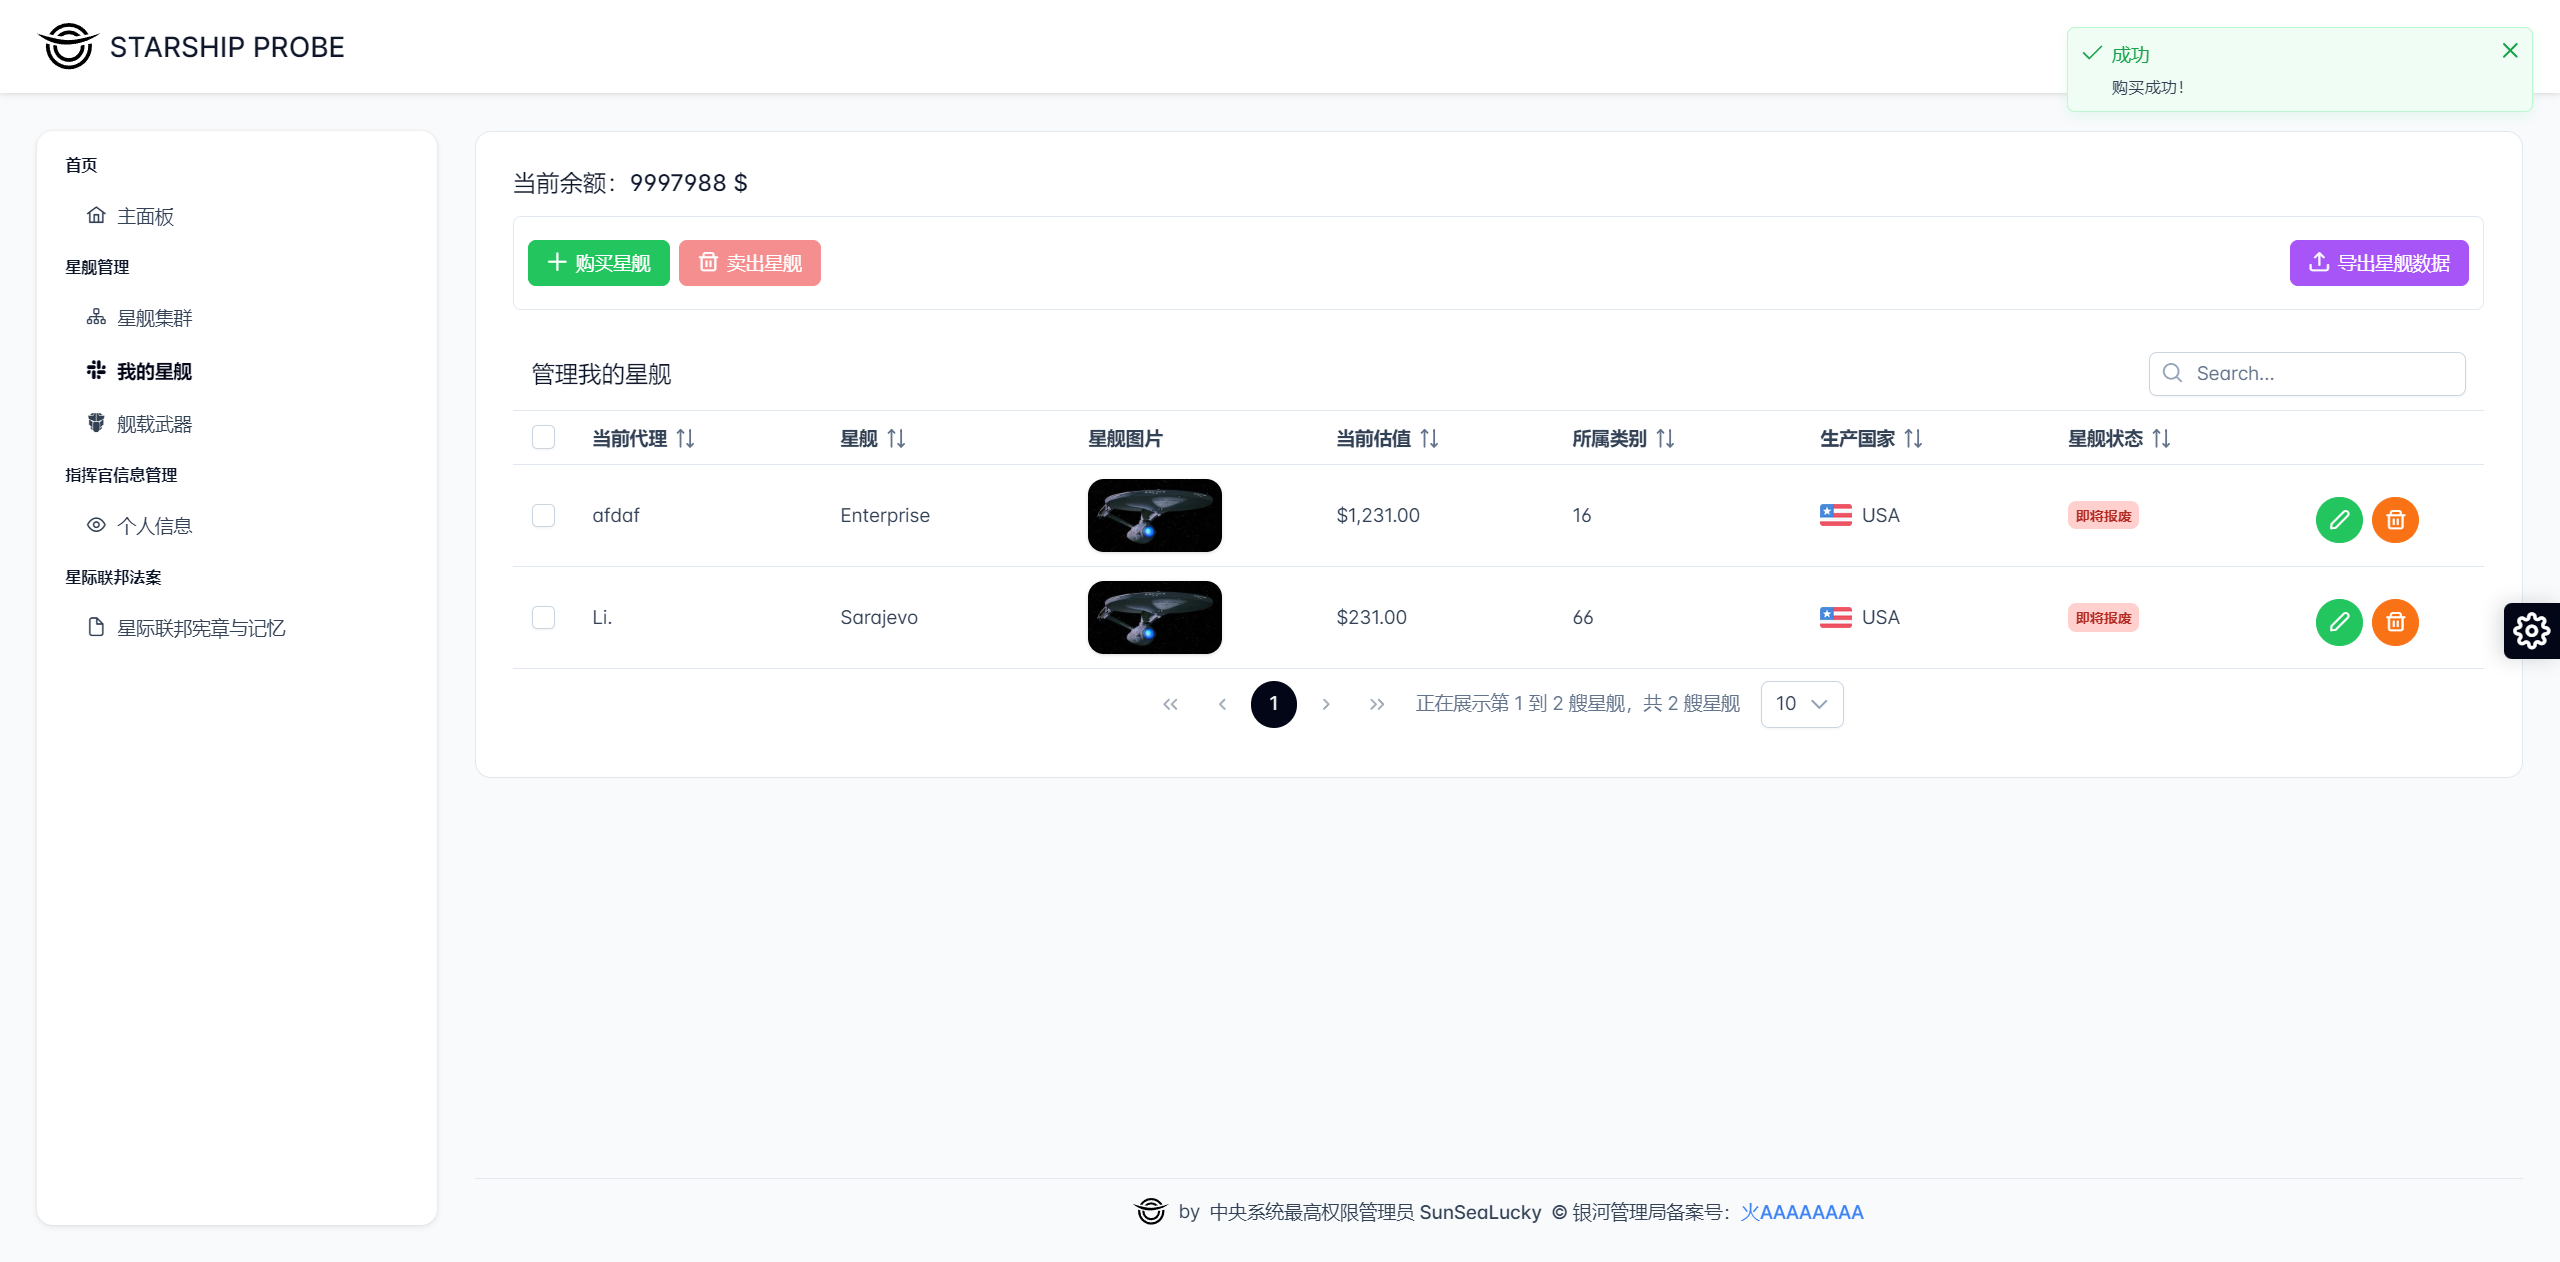
\includegraphics[width=\linewidth]{images/BuyStarshipSuccess}
	\caption{星舰购买成功,右上角弹出提示}
	\label{fig:buystarshipsuccess}
\end{figure}

% TODO: \usepackage{graphicx} required
\begin{figure}[H]
	\centering
	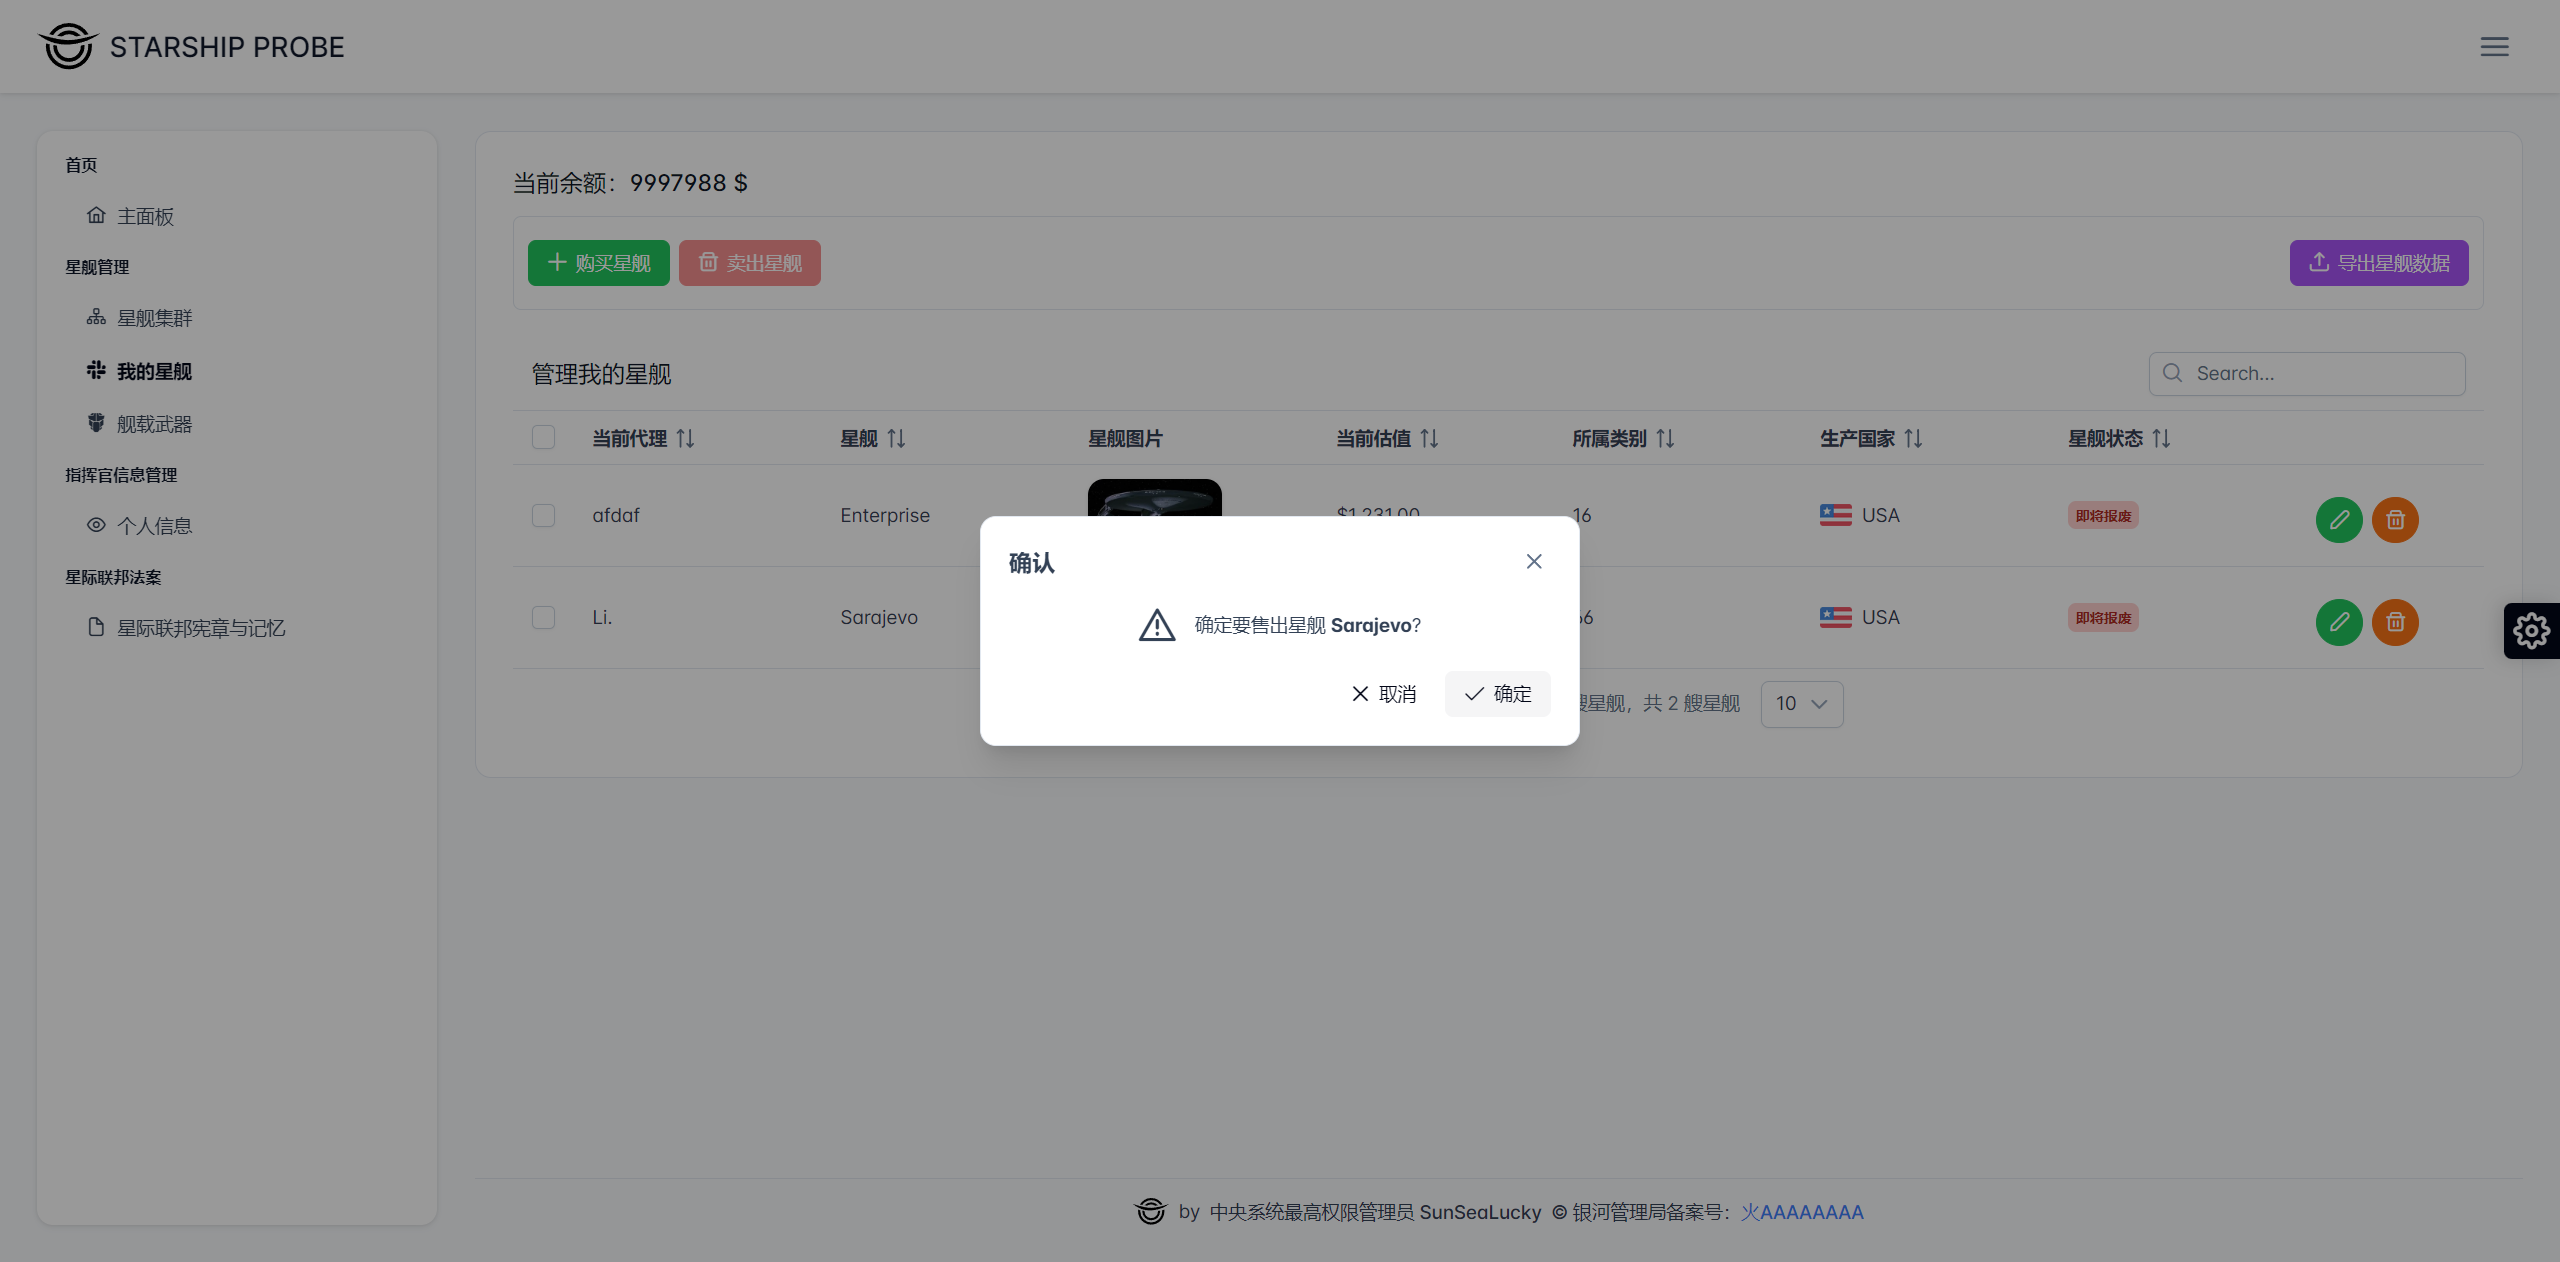
\includegraphics[width=\linewidth]{images/SaleStarship}
	\caption{售出星舰}
	\label{fig:salestarship}
\end{figure}

\subsubsection{武器的管理与购买}

% TODO: \usepackage{graphicx} required
\begin{figure}[H]
	\centering
	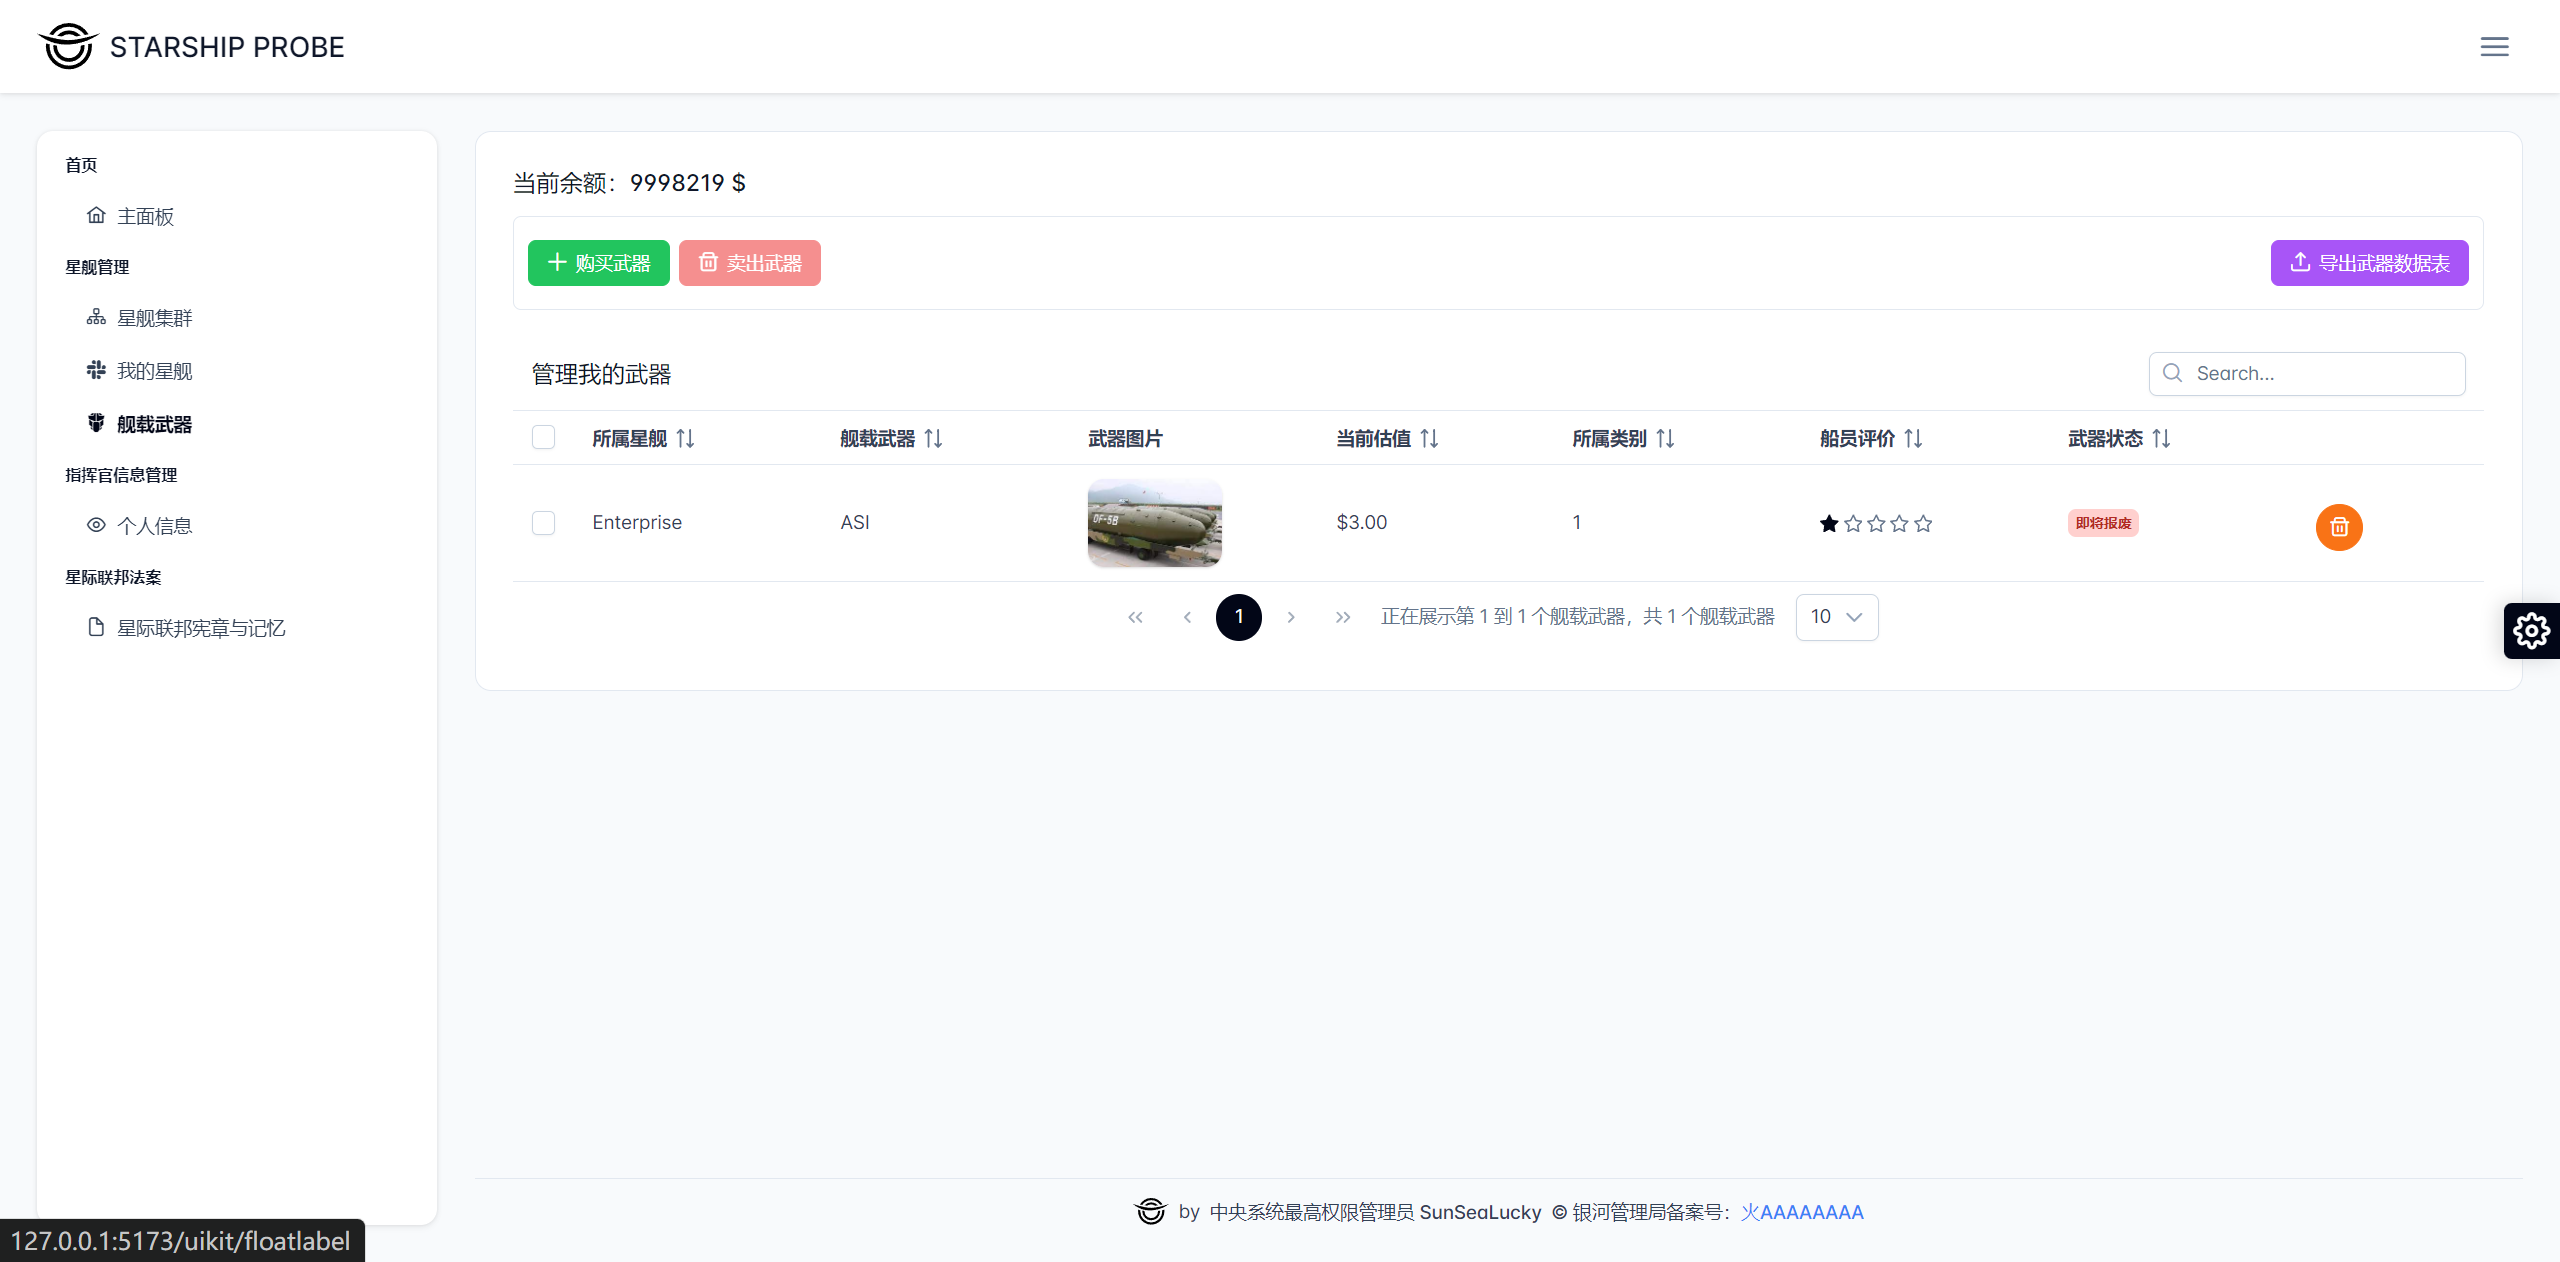
\includegraphics[width=\linewidth]{images/WeaponPage}
	\caption{舰载武器管理界面}
	\label{fig:weaponpage}
\end{figure}

舰载武器的管理与星舰类似,也可以购买或出售,因此不再赘述。只是字段有些不同。

\subsubsection{个人信息的更新}

% TODO: \usepackage{graphicx} required
\begin{figure}[H]
	\centering
	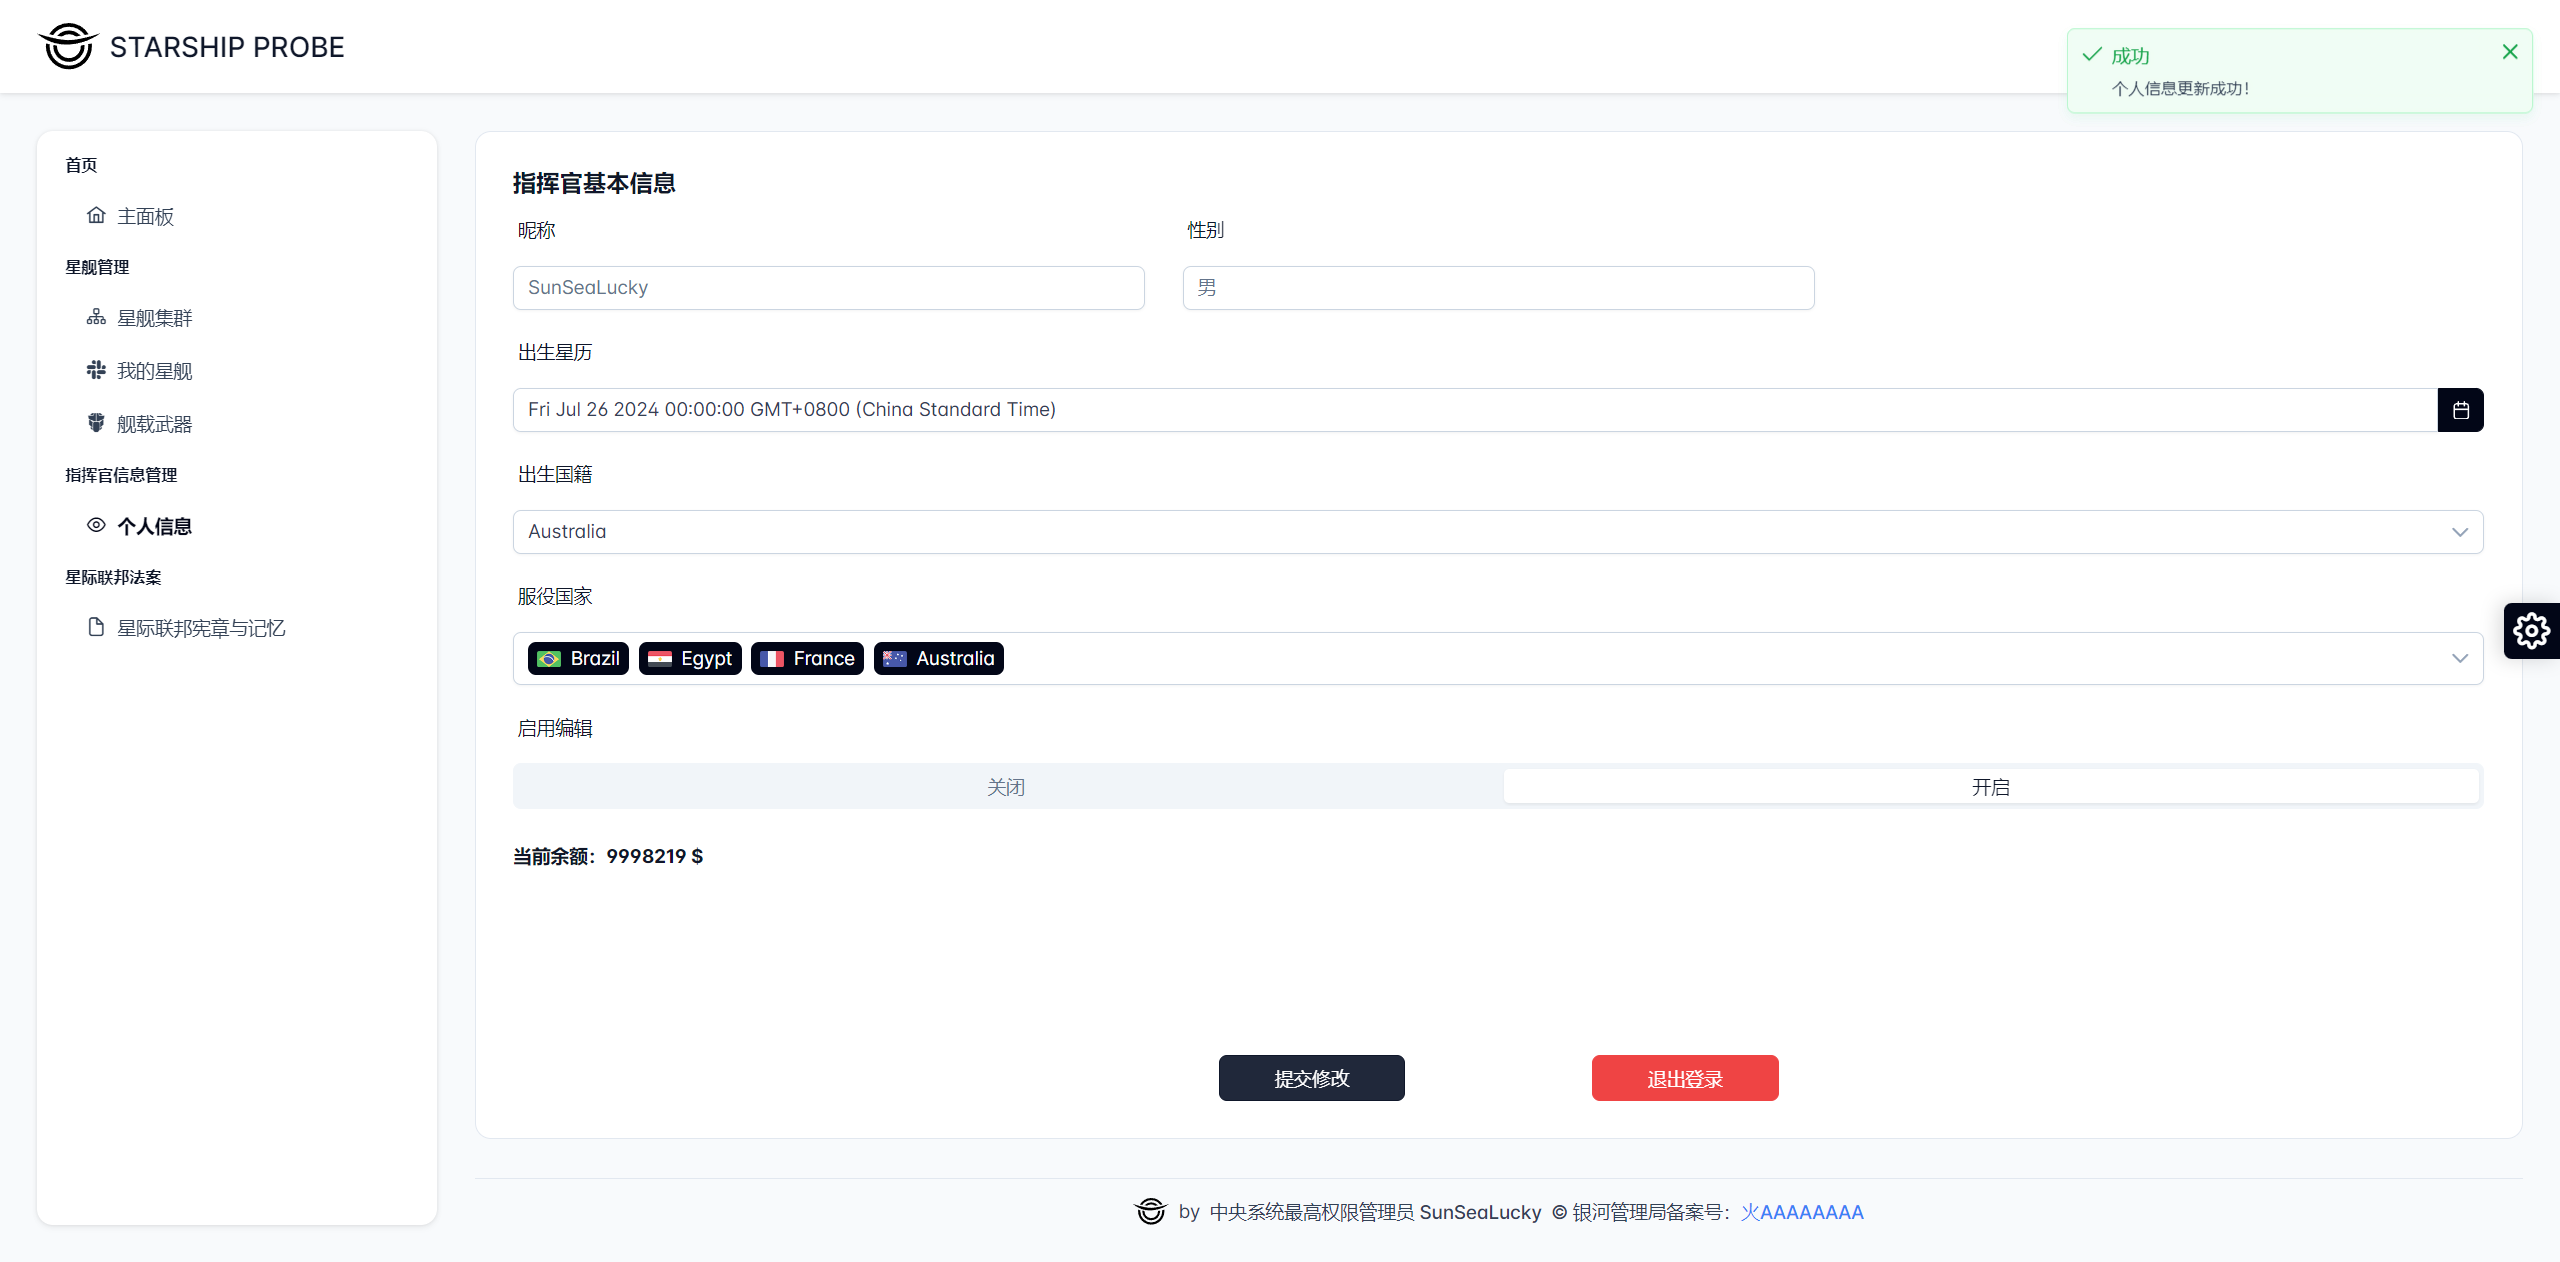
\includegraphics[width=\linewidth]{images/PersonalInformation}
	\caption{个人信息的更新}
	\label{fig:personalinformation}
\end{figure}


昵称、性别、出生日期和出生国籍都是关于指挥官的基本个人信息。服役国家选择为下拉框形式提供给用户,且可多选并带有国家国旗。用户可以选择关闭或者开启手动编辑模式,进行个人信息的更新。

当前余额显示了用户当前的金额,每位用户初始默认有 9999999 \$ 用于购买星舰或者武器。

用户可以通过点击提交修改和退出登录按钮来进行相应的操作,提交对个人信息的修改或者结束当前的登录状态。

整个页面设计简洁明快,采用了蓝色调,各个功能模块划分清晰,易于理解和操作。用户可以根据需要对自己的信息进行修改,并且可以看到自己的余额情况。

个人信息的保存使用 Pinia:
\begin{verbatim}
	import { defineStore } from 'pinia';
	import { ref } from 'vue';
	
	export const useUserStore = defineStore(
	'user',
	() => {
		const username = ref(null);
		const sex = ref(null);
		const born_time = ref(null);
		const born_country = ref(null);
		const serving_country = ref(null);
		const balance = ref(null);
		
		return { username, sex, born_time, 
			born_country, serving_country, balance };
	},
	{
		persist: true
	});
	
\end{verbatim}

\subsubsection{星际联邦宪章与记忆}
% TODO: \usepackage{graphicx} required
\begin{figure}[H]
	\centering
	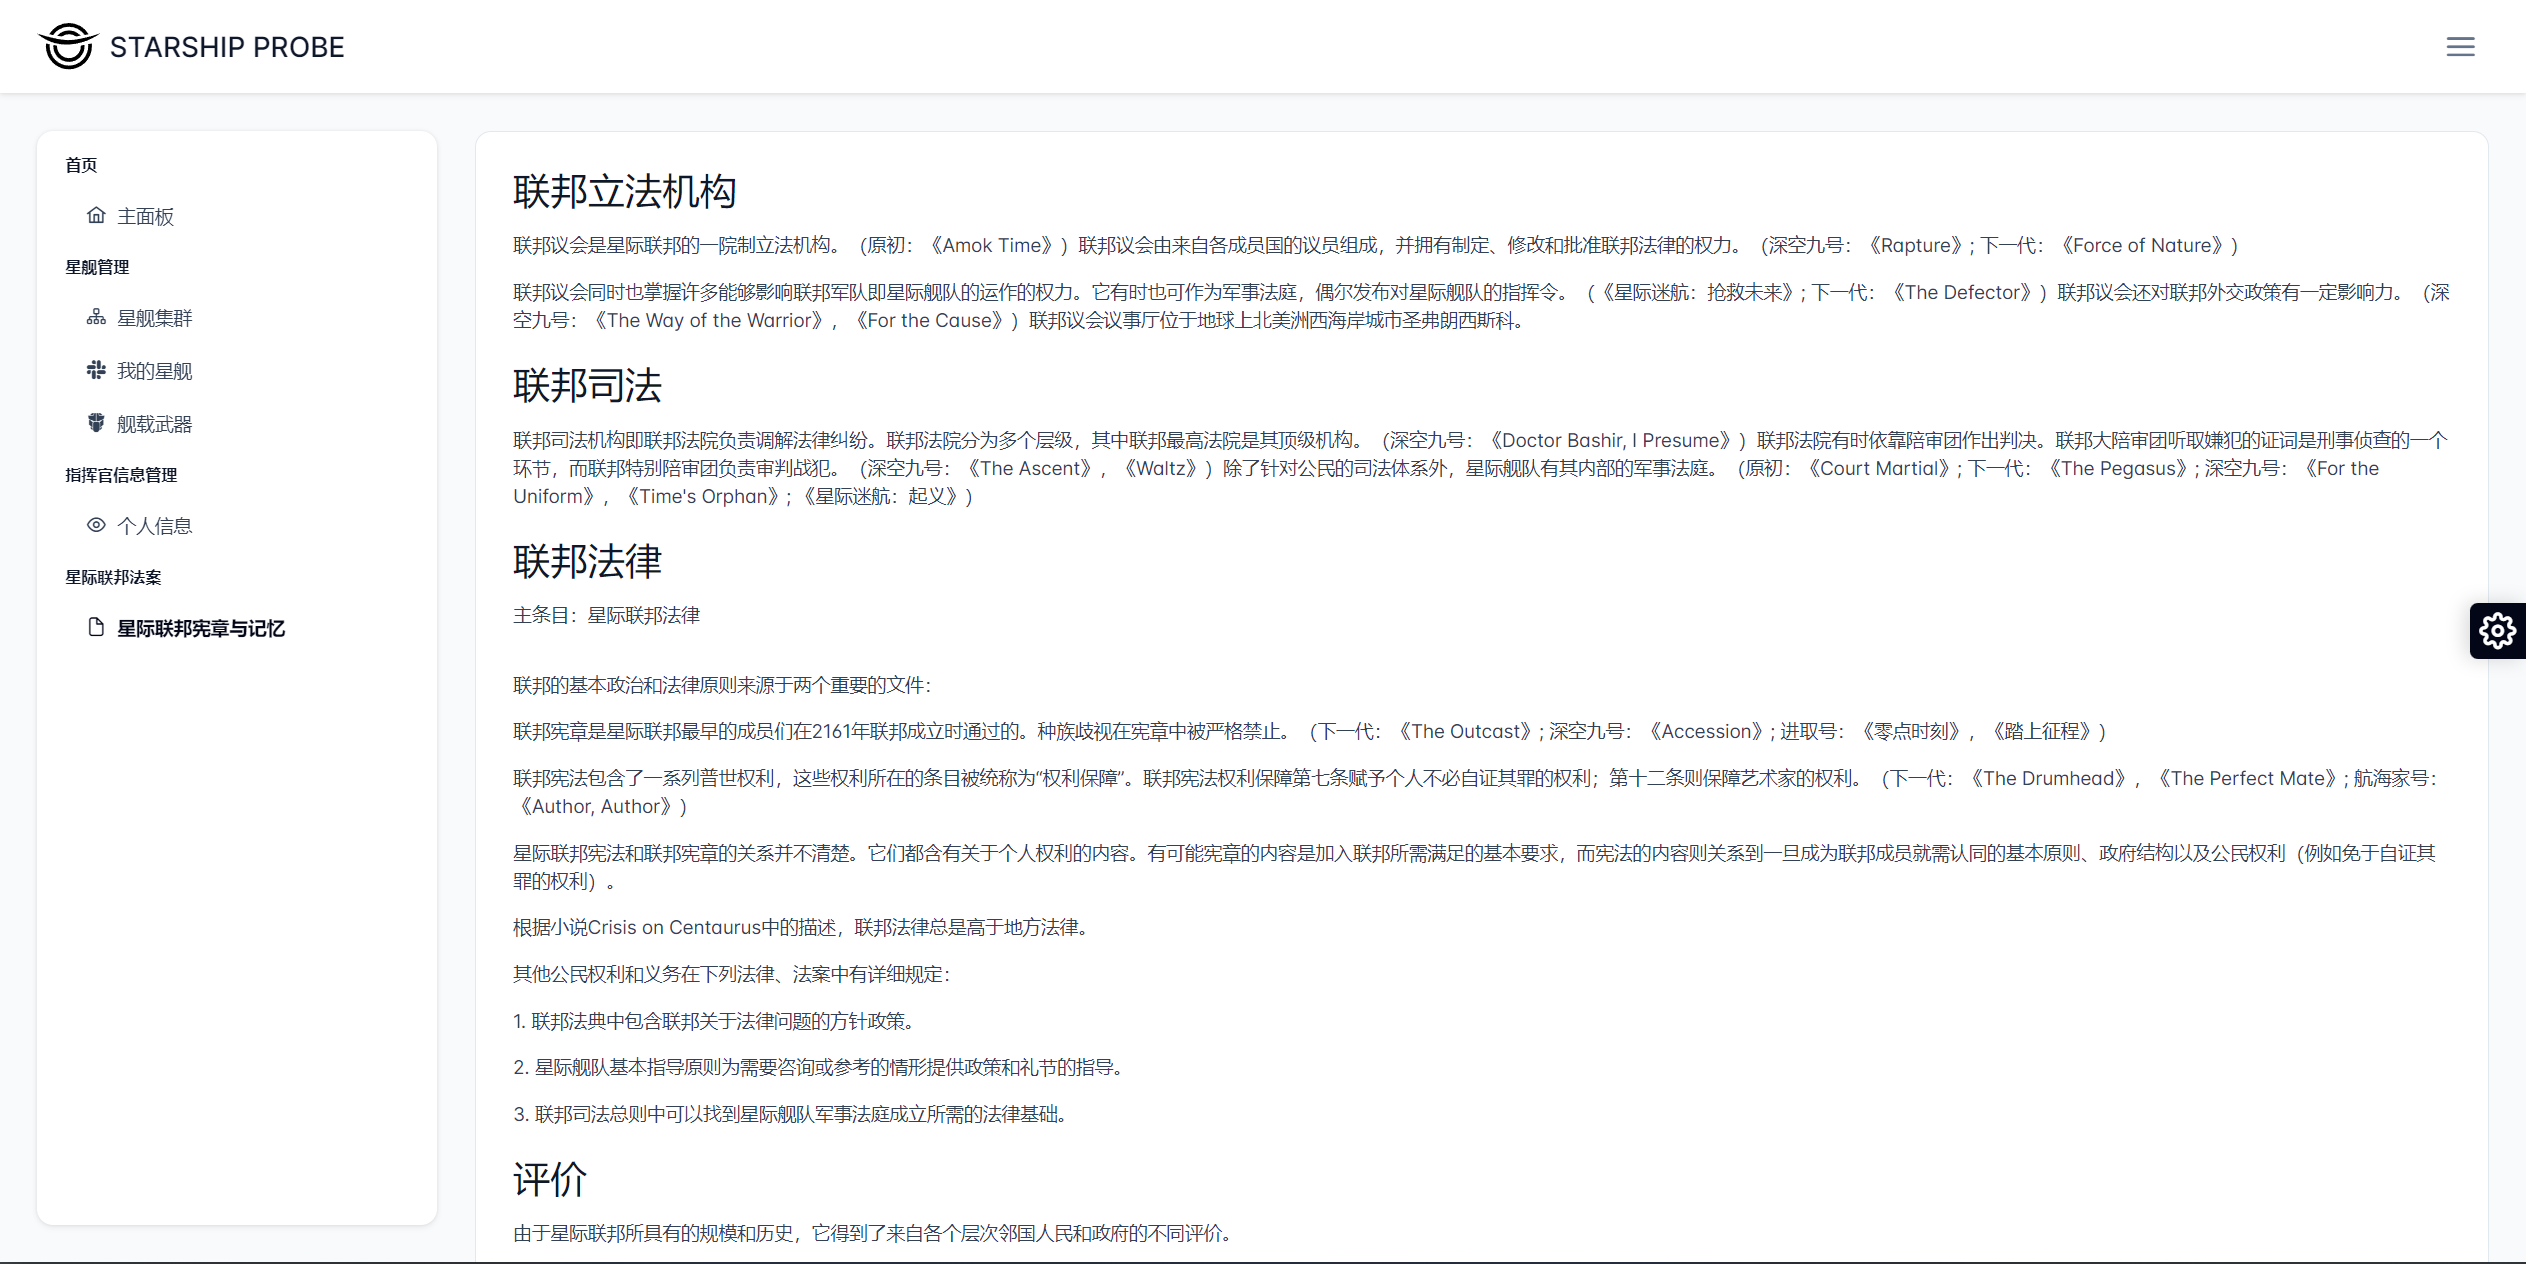
\includegraphics[width=\linewidth]{images/StarLaw}
	\caption{星际联邦宪章与记忆页。仅为展示之用,无与后端交互功能。}
	\label{fig:starlaw}
\end{figure}


\subsubsection{拓展功能}

这个菜单(图 \ref{fig:starlaw})提供了多种视觉和交互方面的自定义选项。用户可以通过拖动滑块来调整界面的缩放级别,以适应不同的屏幕尺寸或个人喜好。可以启用或禁用黑暗模式,这通常有助于减少眼睛疲劳并在低光环境下提供更好的阅读体验。

用户可以选择静态或覆盖类型的菜单显示方式。静态可能表示菜单会固定在某个位置,而覆盖可能意味着菜单会在屏幕上覆盖其他内容。用户可以选择两种不同的输入框样式——包裹型和填充型。这会影响文本框周围的边框和背景颜色。

% TODO: \usepackage{graphicx} required
\begin{figure}[H]
	\centering
	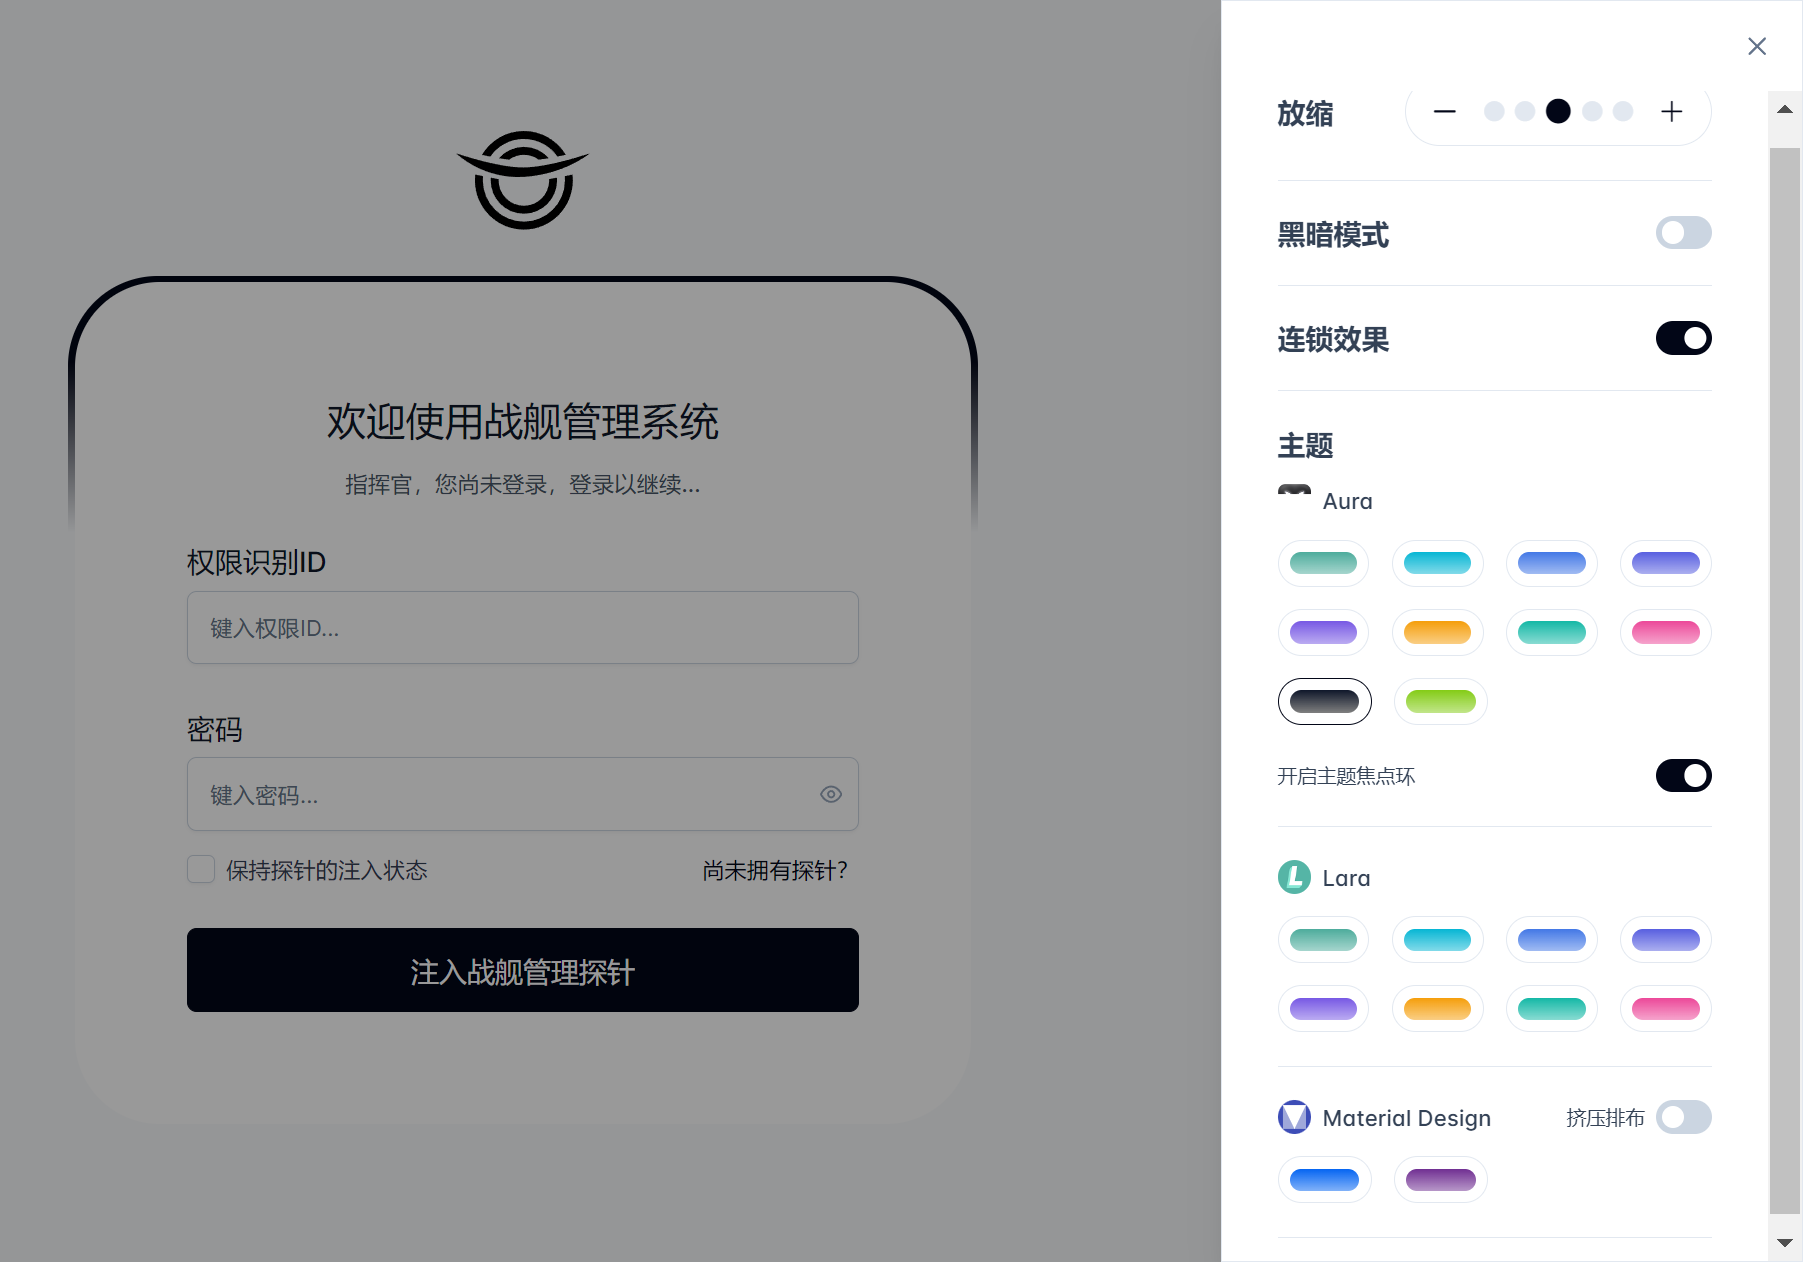
\includegraphics[width=\linewidth]{images/SideBarRight}
	\caption{主题修改栏}
	\label{fig:sidebarright}
\end{figure}

如果启用连锁效果,可能会导致某些操作或事件触发一系列反应或动画。用户可以从三种不同的主题中选择:Aura、Lara 和 Material Design。每个主题都有预览示例,显示了不同颜色方案下的按钮外观。

当启用时开启主题焦点环,可能会显示突出显示当前焦点元素的视觉反馈,这对于键盘导航特别有用。
Lara 主题类似于 Aura,但具有不同的颜色组合。Material Design 主题遵循 Google 的 Material Design 设计规范,提供挤压排布的按钮样式。

这些设置允许用户根据个人喜好定制界面的外观和感觉,提高舒适度和易用性。

\subsection{后端详细设计}

\subsubsection{数据库设计}
数据库设计模式见图 \ref{fig:databaseschema},我使用了 MySQL 自带的 Workbench 绘制了 ER 图,并借助自动生成功能生成了建表的 SQL 语句。

\subsubsection{三层架构}

Spring Boot 是一个流行的 Java 框架,用于快速构建独立的、生产级别的 Spring 应用程序。为了组织代码和实现良好的架构设计,通常采用三层架构:Mapper、Service 和 Controller。每一层各司其职,确保代码的可维护性和可扩展性。

% TODO: \usepackage{graphicx} required
\begin{figure}[H]
	\centering
	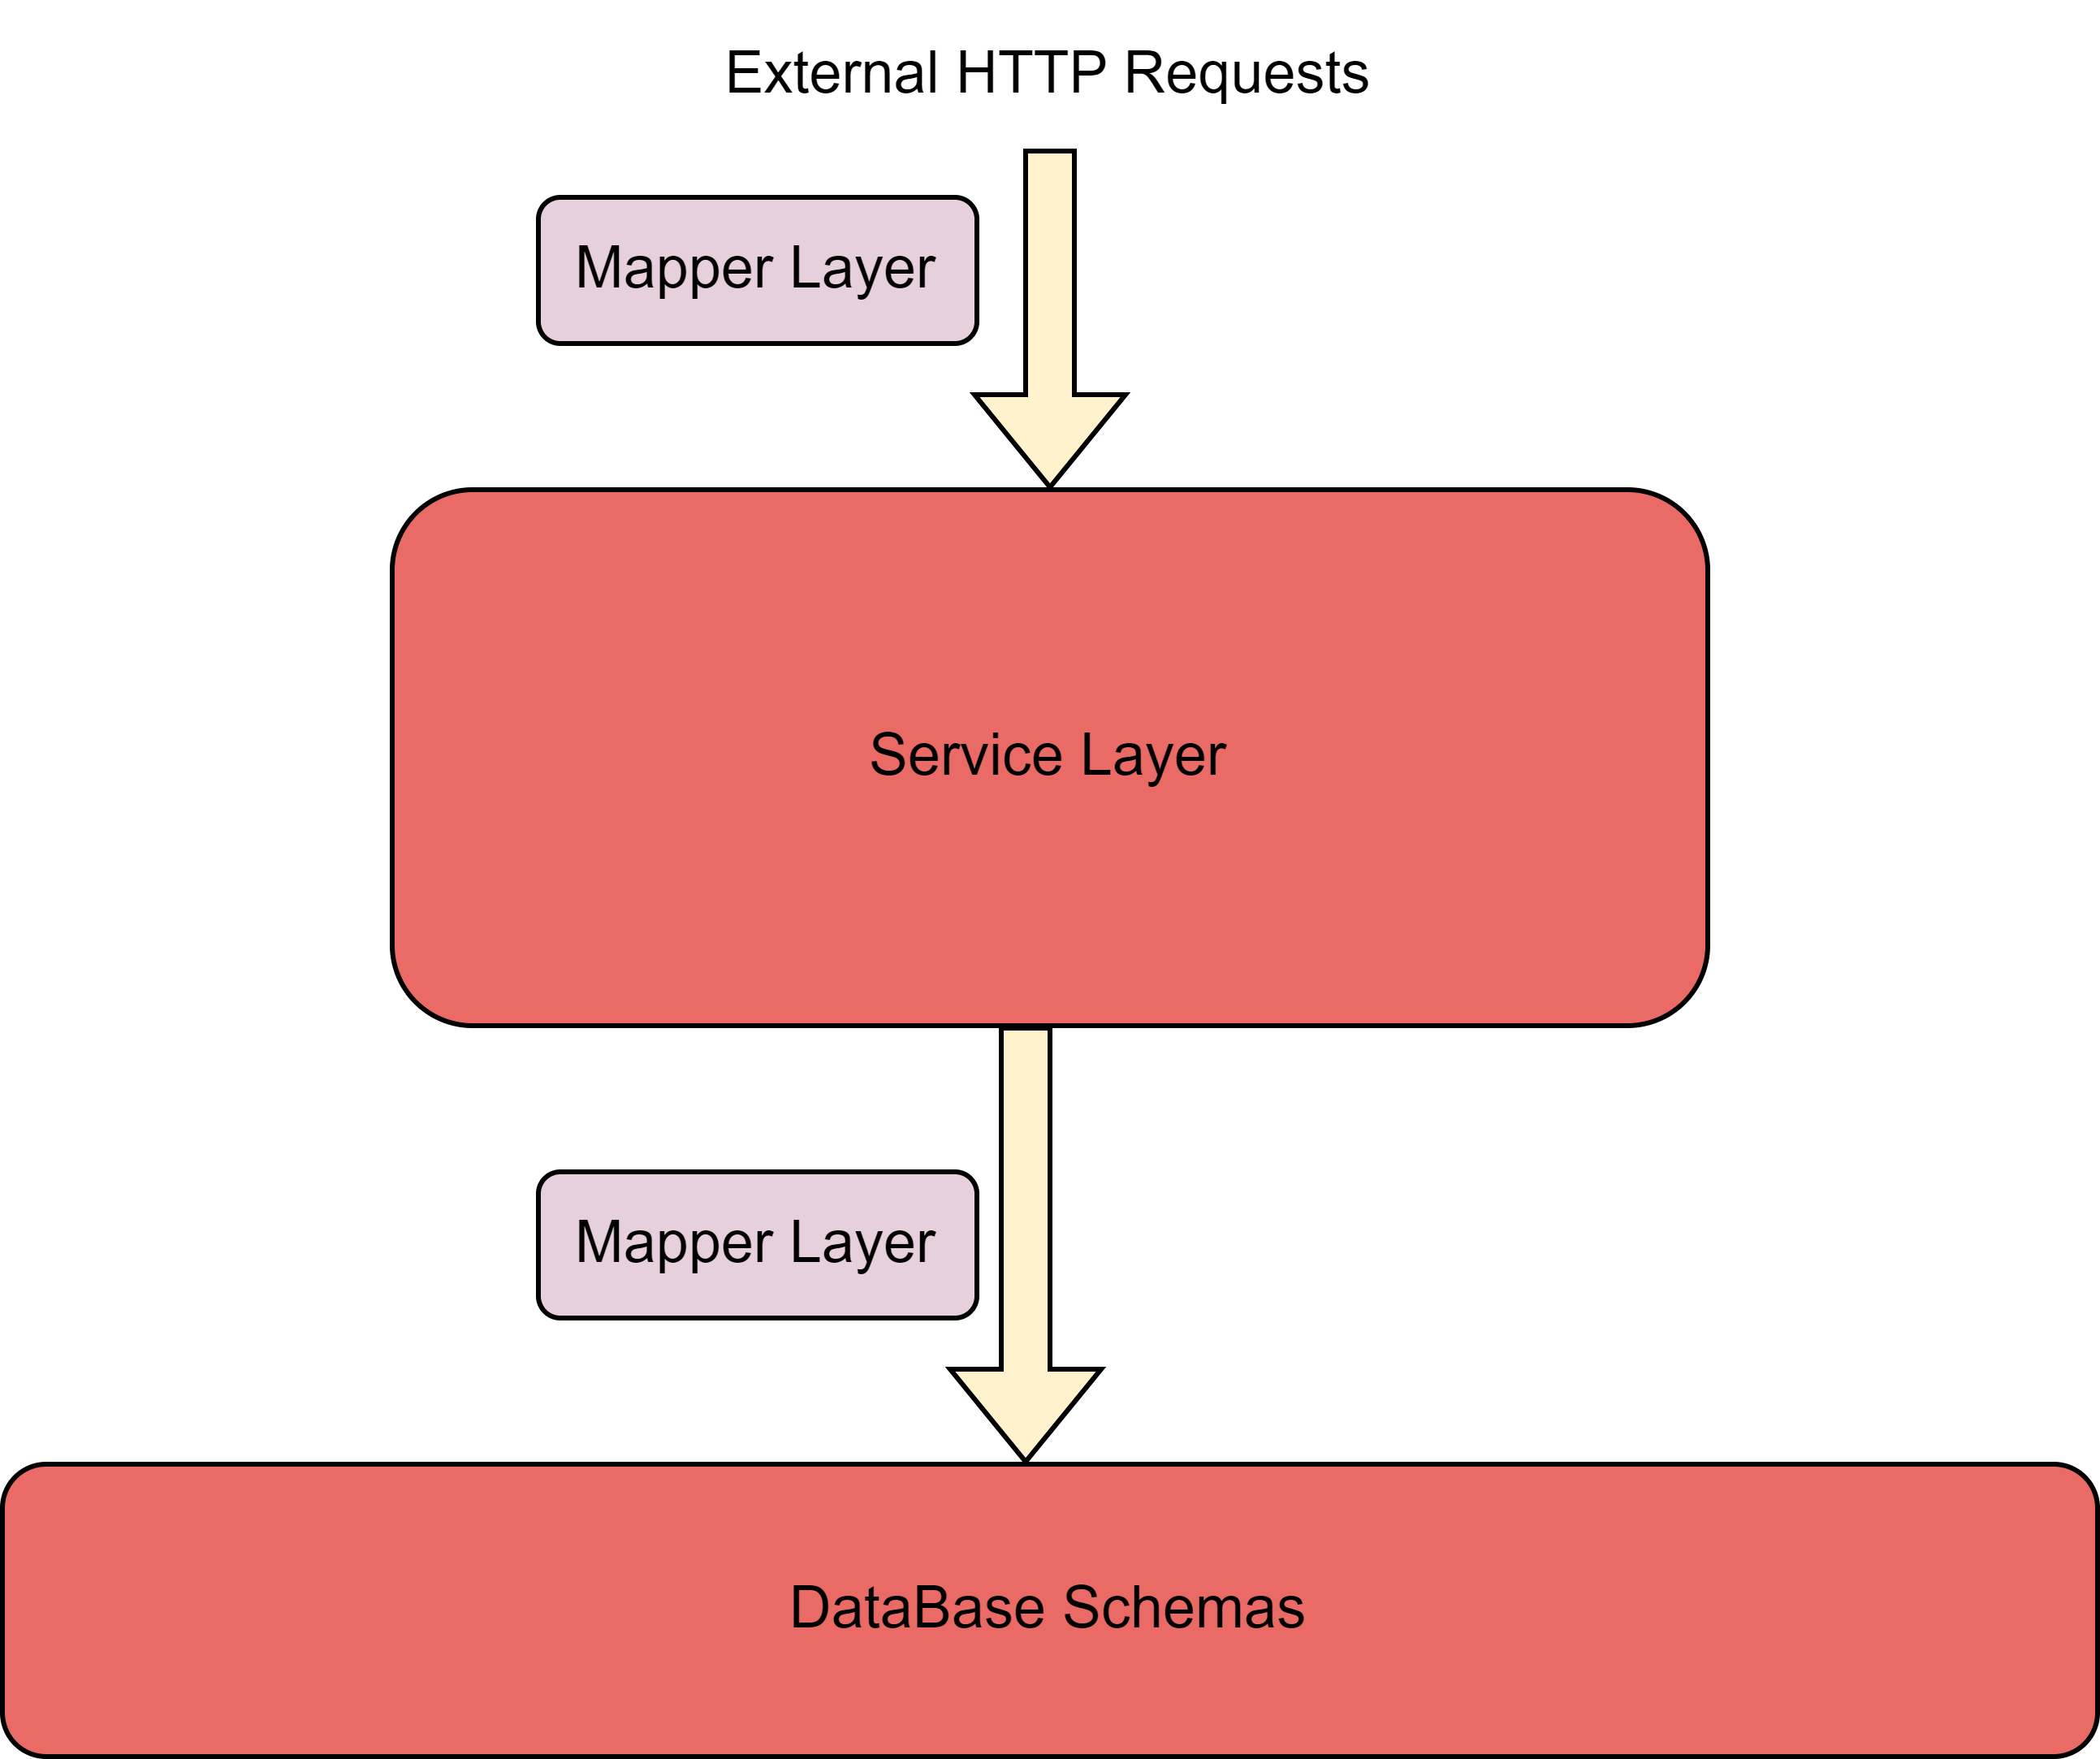
\includegraphics[width=0.7\linewidth]{images/ThreeLayersDesign}
	\caption{三层架构设计}
	\label{fig:threelayersdesign}
\end{figure}

\textbf{Controller 层} 处理 HTTP 请求和响应。负责接收客户端的请求,调用服务层进行业务处理,然后返回结果给客户端。

\textbf{Service 层} 处理业务逻辑。包含具体的业务规则和逻辑操作,调用数据访问层来获取和存储数据。

\textbf{Mapper 层} 数据访问层,负责与数据库进行交互。通常使用 MyBatis 或 JPA 等框架进行数据库操作。

三层架构具有许多优点,一是可以分离关注点,每一层只关注自己的职责,降低了代码的耦合度;二是使代码更容易阅读和维护,因为逻辑清晰分层;三是各层的修改不会影响到其他层,便于功能扩展和修改;四是每一层都专注于处理特定的任务,提高了代码质量和可靠性。

% TODO: \usepackage{graphicx} required
\begin{figure}[H]
	\centering
	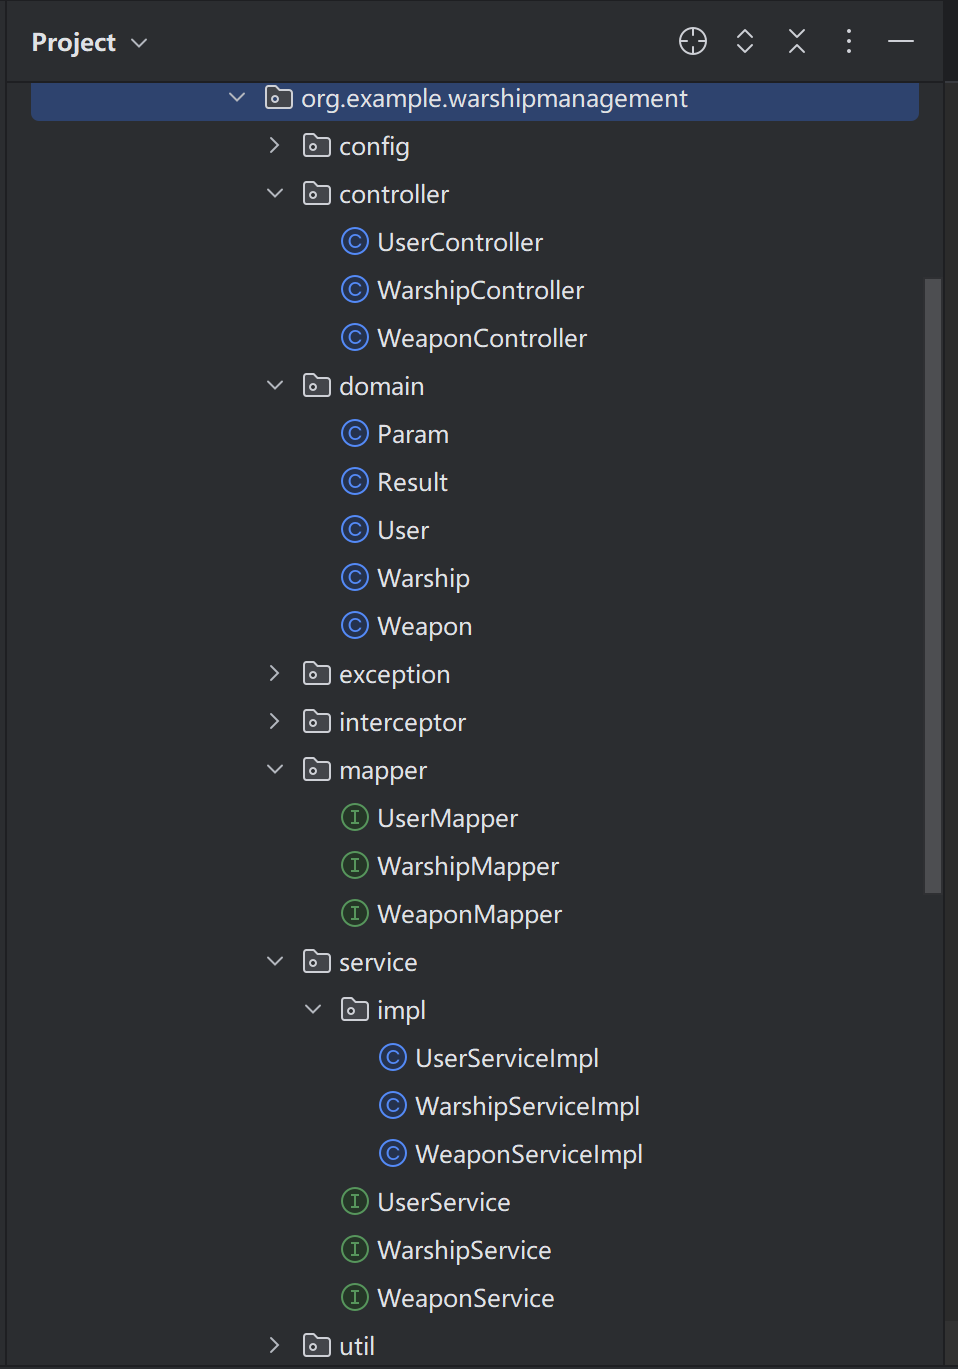
\includegraphics[width=0.7\linewidth]{images/BackEndProjectStructure}
	\caption{后端基本结构图}
	\label{fig:backendprojectstructure}
\end{figure}


\subsubsection{Controller,控制层}

在 Spring Boot 框架中,Controller 层是 MVC(Model-View-Controller)架构模式中的控制器部分,它是应用程序中处理 HTTP 请求和生成响应的主要组件。

Controller 层使用注解如 @RequestMapping, @GetMapping, @PostMapping 等来关联特定的 HTTP 请求(如 GET, POST, PUT, DELETE 等)到具体的方法。这使得 URL 路径和请求方法能够被映射到应用程序内的特定处理函数。

当请求到达时,Controller层负责解析请求中的参数,包括 URL 路径参数(使用 @PathVariable)、查询字符串参数(使用 @RequestParam)、请求体中的数据(使用 @RequestBody)以及从 HTTP 头中提取的信息。

\textbf{Controller 层不包含复杂的业务逻辑,而是作为中介,调用Service层的方法来执行实际的业务处理}。这样做的好处是将关注点分离,使得 Controller 层专注于请求处理和响应生成,而业务逻辑则由 Service 层管理。

% TODO: \usepackage{graphicx} required
\begin{figure}[H]
	\centering
	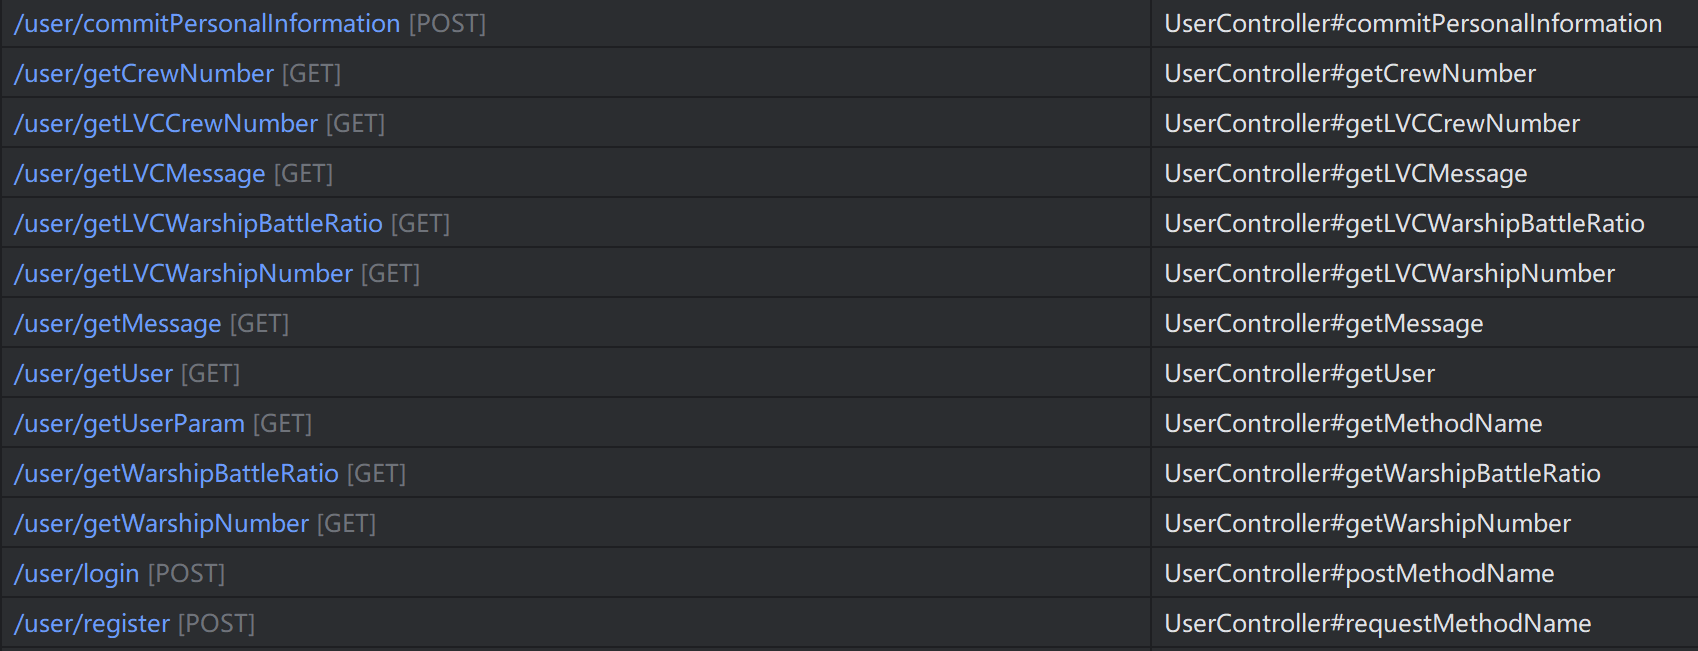
\includegraphics[width=\linewidth]{images/UserController}
	\caption{UserController 下的 Mappings}
	\label{fig:usercontroller}
\end{figure}

% TODO: \usepackage{graphicx} required
\begin{figure}[H]
	\centering
	\includegraphics[width=\linewidth]{"images/WarshipController & Weapon Controller"}
	\caption{Warship Controller 和 Weapon Controller 下的 Mappings}
	\label{fig:warshipcontroller--weapon-controller}
\end{figure}

Controller 层负责将 Service 层返回的数据封装成适当的格式,如 JSON、XML 或 HTML,以便通过 HTTP 响应发送回客户端。这通常通过 @ResponseBody 或 @RestController 注解来完成。

如果应用程序使用模板引擎(如 Thymeleaf 或 FreeMarker ),Controller 层会将数据模型传递给视图层,视图层负责将数据渲染成最终的HTML页面。

Controller 层可以处理运行时发生的异常,并通过 @ExceptionHandler 注解来定义异常处理器,以确保应用程序在出现错误时能够优雅地响应,例如返回错误信息或重定向到错误页面。

Controller 层可以集成安全框架,如 Spring Security,来处理用户身份验证和授权,确保只有经过适当认证的用户才能访问特定的资源。
在Spring Boot中,Controller 类通常会被标记为 @Controller 或 @RestController,后者隐含了 @ResponseBody 的行为,即所有方法的返回值都将直接写入 HTTP 响应体,而不是转发到视图。

\subsubsection{Domain,实体层}
从图 \ref{fig:backendprojectstructure} 中可以看出,除了本项目必要的三个实体(用户、星舰、武器)之外,还有 Param 和 Result 两个实体。他们并不绑定数据库表,而仅仅做返回对象之用。

Result 用于返回响应结果:
\begin{verbatim}
	@NoArgsConstructor
	@AllArgsConstructor
	@Data
	public class Result<T> {
		private T data;
		private int code;
		private String msg;
		
		public static <E> Result<E> success(E data) {
			return new Result<E>(data, 200, "Response success!");
		}
		
		public static Result<String> success(String data) {
			return new Result<String>(data, 200, "Response success!");
		}
		
		public static Result<User> fail(String msg) {
			return new Result<User>(null, 100, msg);
		}
	}
\end{verbatim}

Param 用于响应登录时的“盐”查询;
\begin{verbatim}
	@AllArgsConstructor
	@NoArgsConstructor
	@Data
	public class Param {
		private String random;
		private String time;
	}
\end{verbatim}


\subsubsection{Service,服务层}

在 Spring Boot 应用中,Service 层是实现业务逻辑的关键部分。它位于 Controller 层和数据访问层(通常是 Repository 或 DAO 层)之间,主要职责是处理业务规则和流程。

Service 层封装了应用程序的核心业务逻辑。它包含了对数据的复杂操作,如计算、数据转换、数据验证以及多个数据源之间的协调等。

Service 层通常调用 Repository 或 DAO 层的方法来存取数据库。当一个业务操作涉及到多个数据表或多个数据访问点时,Service 层会协调这些操作,保证它们按正确的顺序和方式执行。

Service 层常常用 @Transactional 注解来管理数据库操作的事务边界。这意味着一系列的操作被视为一个整体,如果其中任何一步失败,所有更改都将被回滚,以保持数据的一致性。

Service 层负责对从 Controller 层接收到的数据进行验证,确保数据符合预期的格式和业务规则。这包括数据完整性检查、格式校验以及业务规则的遵守。

Service 层可能需要将一种格式的数据转换为另一种格式,以便于存储或展示。例如,将用户输入转换为数据库可识别的格式,或将数据库数据转换为适合前端显示的格式。

Service 层可以定义接口,从而隐藏底层实现细节。这有助于代码的模块化和可测试性,同时也允许 Service 层的实现可以更容易地被替换或升级。

Service 层的方法通常设计为可复用的,这意味着它们可以被不同的 Controller 或其他 Service 层调用,减少了代码冗余,提高了代码的可维护性。

对于耗时较长的任务,如文件上传、邮件发送或复杂的计算,Service 层可以利用异步编程模型,如 Spring 的 @Async 注解,来异步执行这些任务,从而提升应用程序的响应速度。

Service 层通常记录重要的业务操作,如交易、用户行为或系统事件,以便于审计和故障排查。

Service 层还可能涉及权限检查和安全策略的实施,以确保只有授权的用户或角色可以执行某些操作。

Service 层是 Spring Boot 应用程序中业务逻辑的集中体现,它确保了业务需求的正确实现,并且通过将业务逻辑与数据访问和表示层分离,提高了系统的灵活性和可维护性。

下面是用户登录时,本项目 Service 层执行的操作:
\begin{verbatim}
	@Override
	public User login(String username, String time, String random, String sign) {
		
		if (findUserByName(username) == null)
		return null;
		
		User u = findUserByName(username);
		
		if (!HashHelper.Hash(u.getPassword() + time + random).equals(sign)) {
			return null;
		}
		
		return u;
	}
\end{verbatim}

\subsubsection{Mapper,数据对象访问层}

在 Spring Boot 和许多其他基于 Java 的企业级应用中,Mapper 层(有时也称为 DAO 层,Data Access Object)是一个专门用于数据访问和数据持久化的层次。特别是在使用 MyBatis 这样的对象关系映射(ORM)框架时,Mapper 层的作用尤为突出。

Mapper 层负责将应用中的实体对象(Entity)持久化到数据库中,以及从数据库中检索数据并将之转化为实体对象。这是通过执行 SQL 语句来实现的,这些 SQL 语句通常是在 XML 配置文件中定义的(在 MyBatis 中)或者直接在代码中编写(在 JPA 或 Hibernate 中)。

在 MyBatis 中,Mapper 层通常与 XML 文件中的 SQL 语句相对应,这些 SQL 语句被映射到特定的 Java 接口方法上。这样可以将 SQL 语句从 Java 代码中分离出来,提高代码的可读性和可维护性。

Mapper 层实现了数据的增(Insert)、删(Delete)、改(Update)和查(Select)操作,简称 CRUD 操作。这些操作是通过与数据库交互来完成的。

Mapper 层将数据库表中的字段与Java实体类中的属性相匹配,也就是进行对象关系映射(ORM)。这样,开发人员可以更自然地使用Java对象来处理数据库数据,而不需要直接处理SQL语句。

虽然事务控制通常在 Service 层处理,但 Mapper 层的操作可能触发事务开始、提交或回滚。在 MyBatis 中,事务控制可以通过编程式或声明式的方式实现。

Mapper层通常表现为一个接口,定义了一系列数据库操作的方法,如 selectList(), insert(), update(), delete() 等。

实际的数据库操作是由框架根据接口方法和对应的 SQL 语句来执行的。在 MyBatis 中,这通常通过在 XML 配置文件中定义 SQL 语句和结果映射来实现。

Mapper 层通常被 Service 层调用,Service 层负责处理业务逻辑,而 Mapper 层则负责数据访问。这种分层架构有助于将业务逻辑与数据访问分离,提高了代码的可读性、可维护性和可测试性。

Mapper 层是 Spring Boot 应用中负责与数据库交互的层次,通过对象关系映射技术,它提供了对数据库的访问和数据的持久化能力,同时通过分层设计保持了代码的清晰和模块化。

% TODO: \usepackage{graphicx} required
\begin{figure}[H]
	\centering
	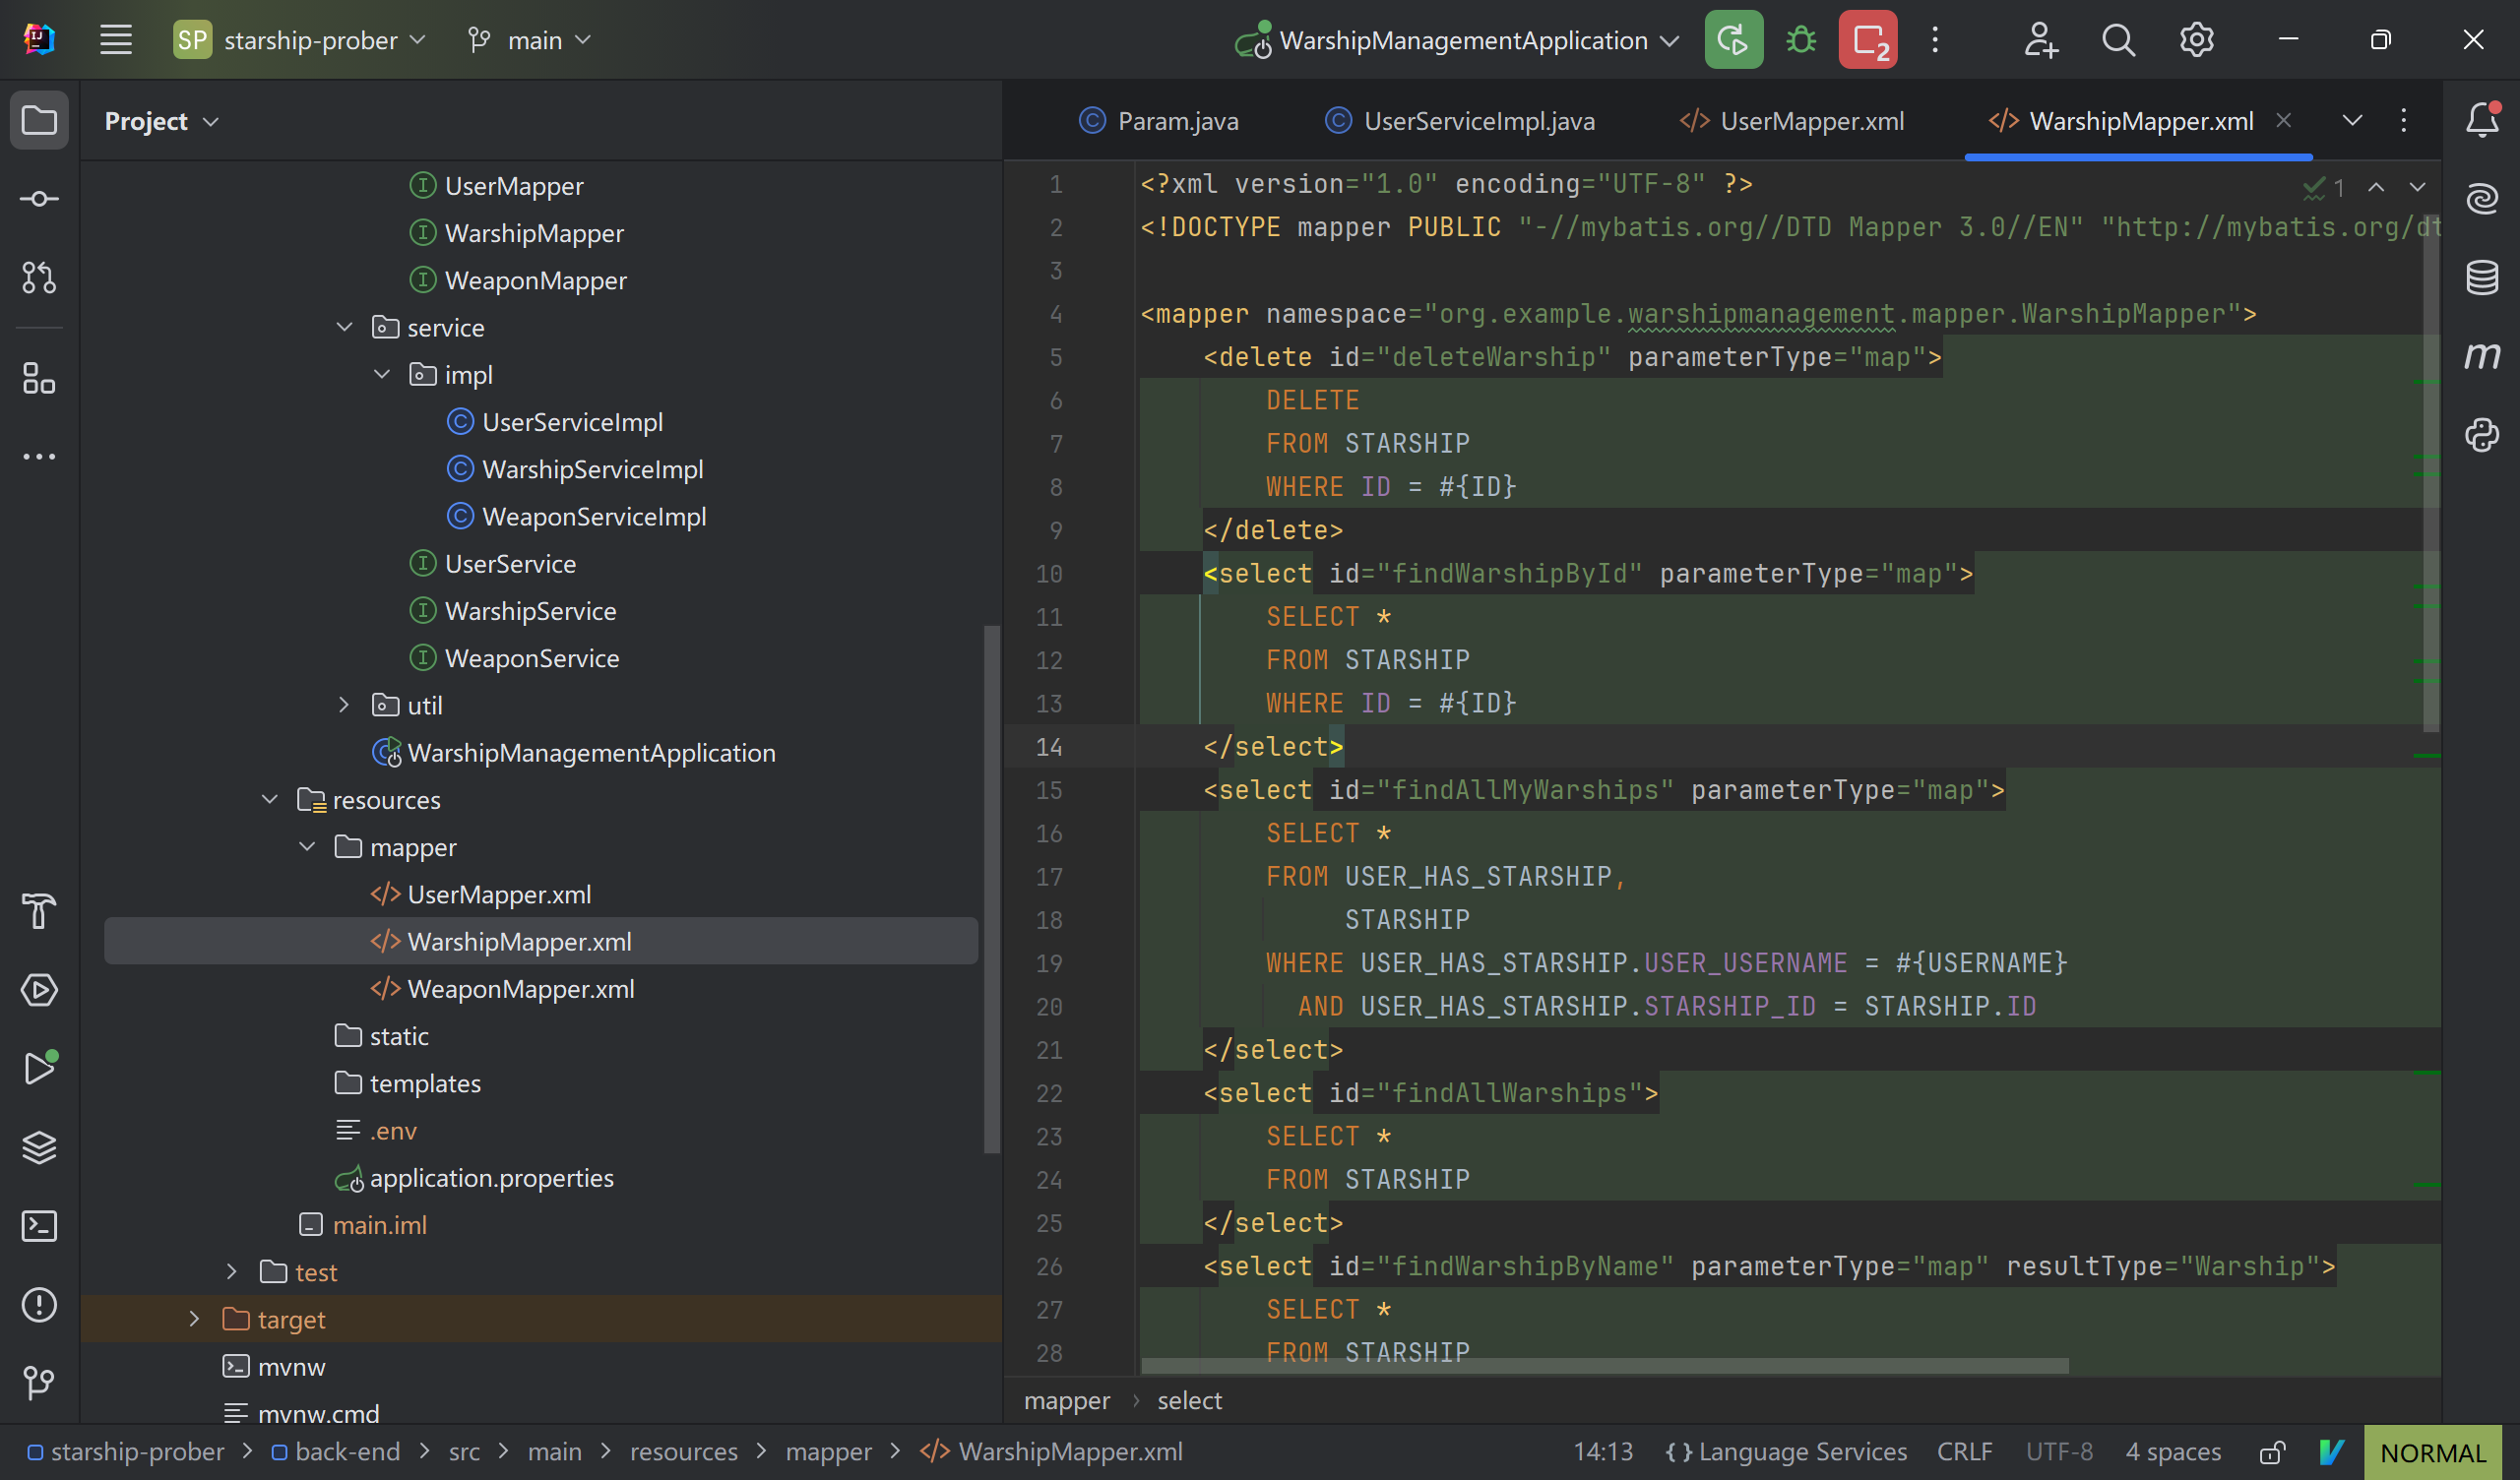
\includegraphics[width=\linewidth]{images/MapperLayer}
	\caption{本项目 Mapper 层的大量 SQL 语句}
	\label{fig:mapperlayer}
\end{figure}

\section{系统测试}
在测试时,后端采用我采用 PostMan 进行测试,前端则直接使用浏览器控制台进行测试已经足够。

% TODO: \usepackage{graphicx} required
\begin{figure}[H]
	\centering
	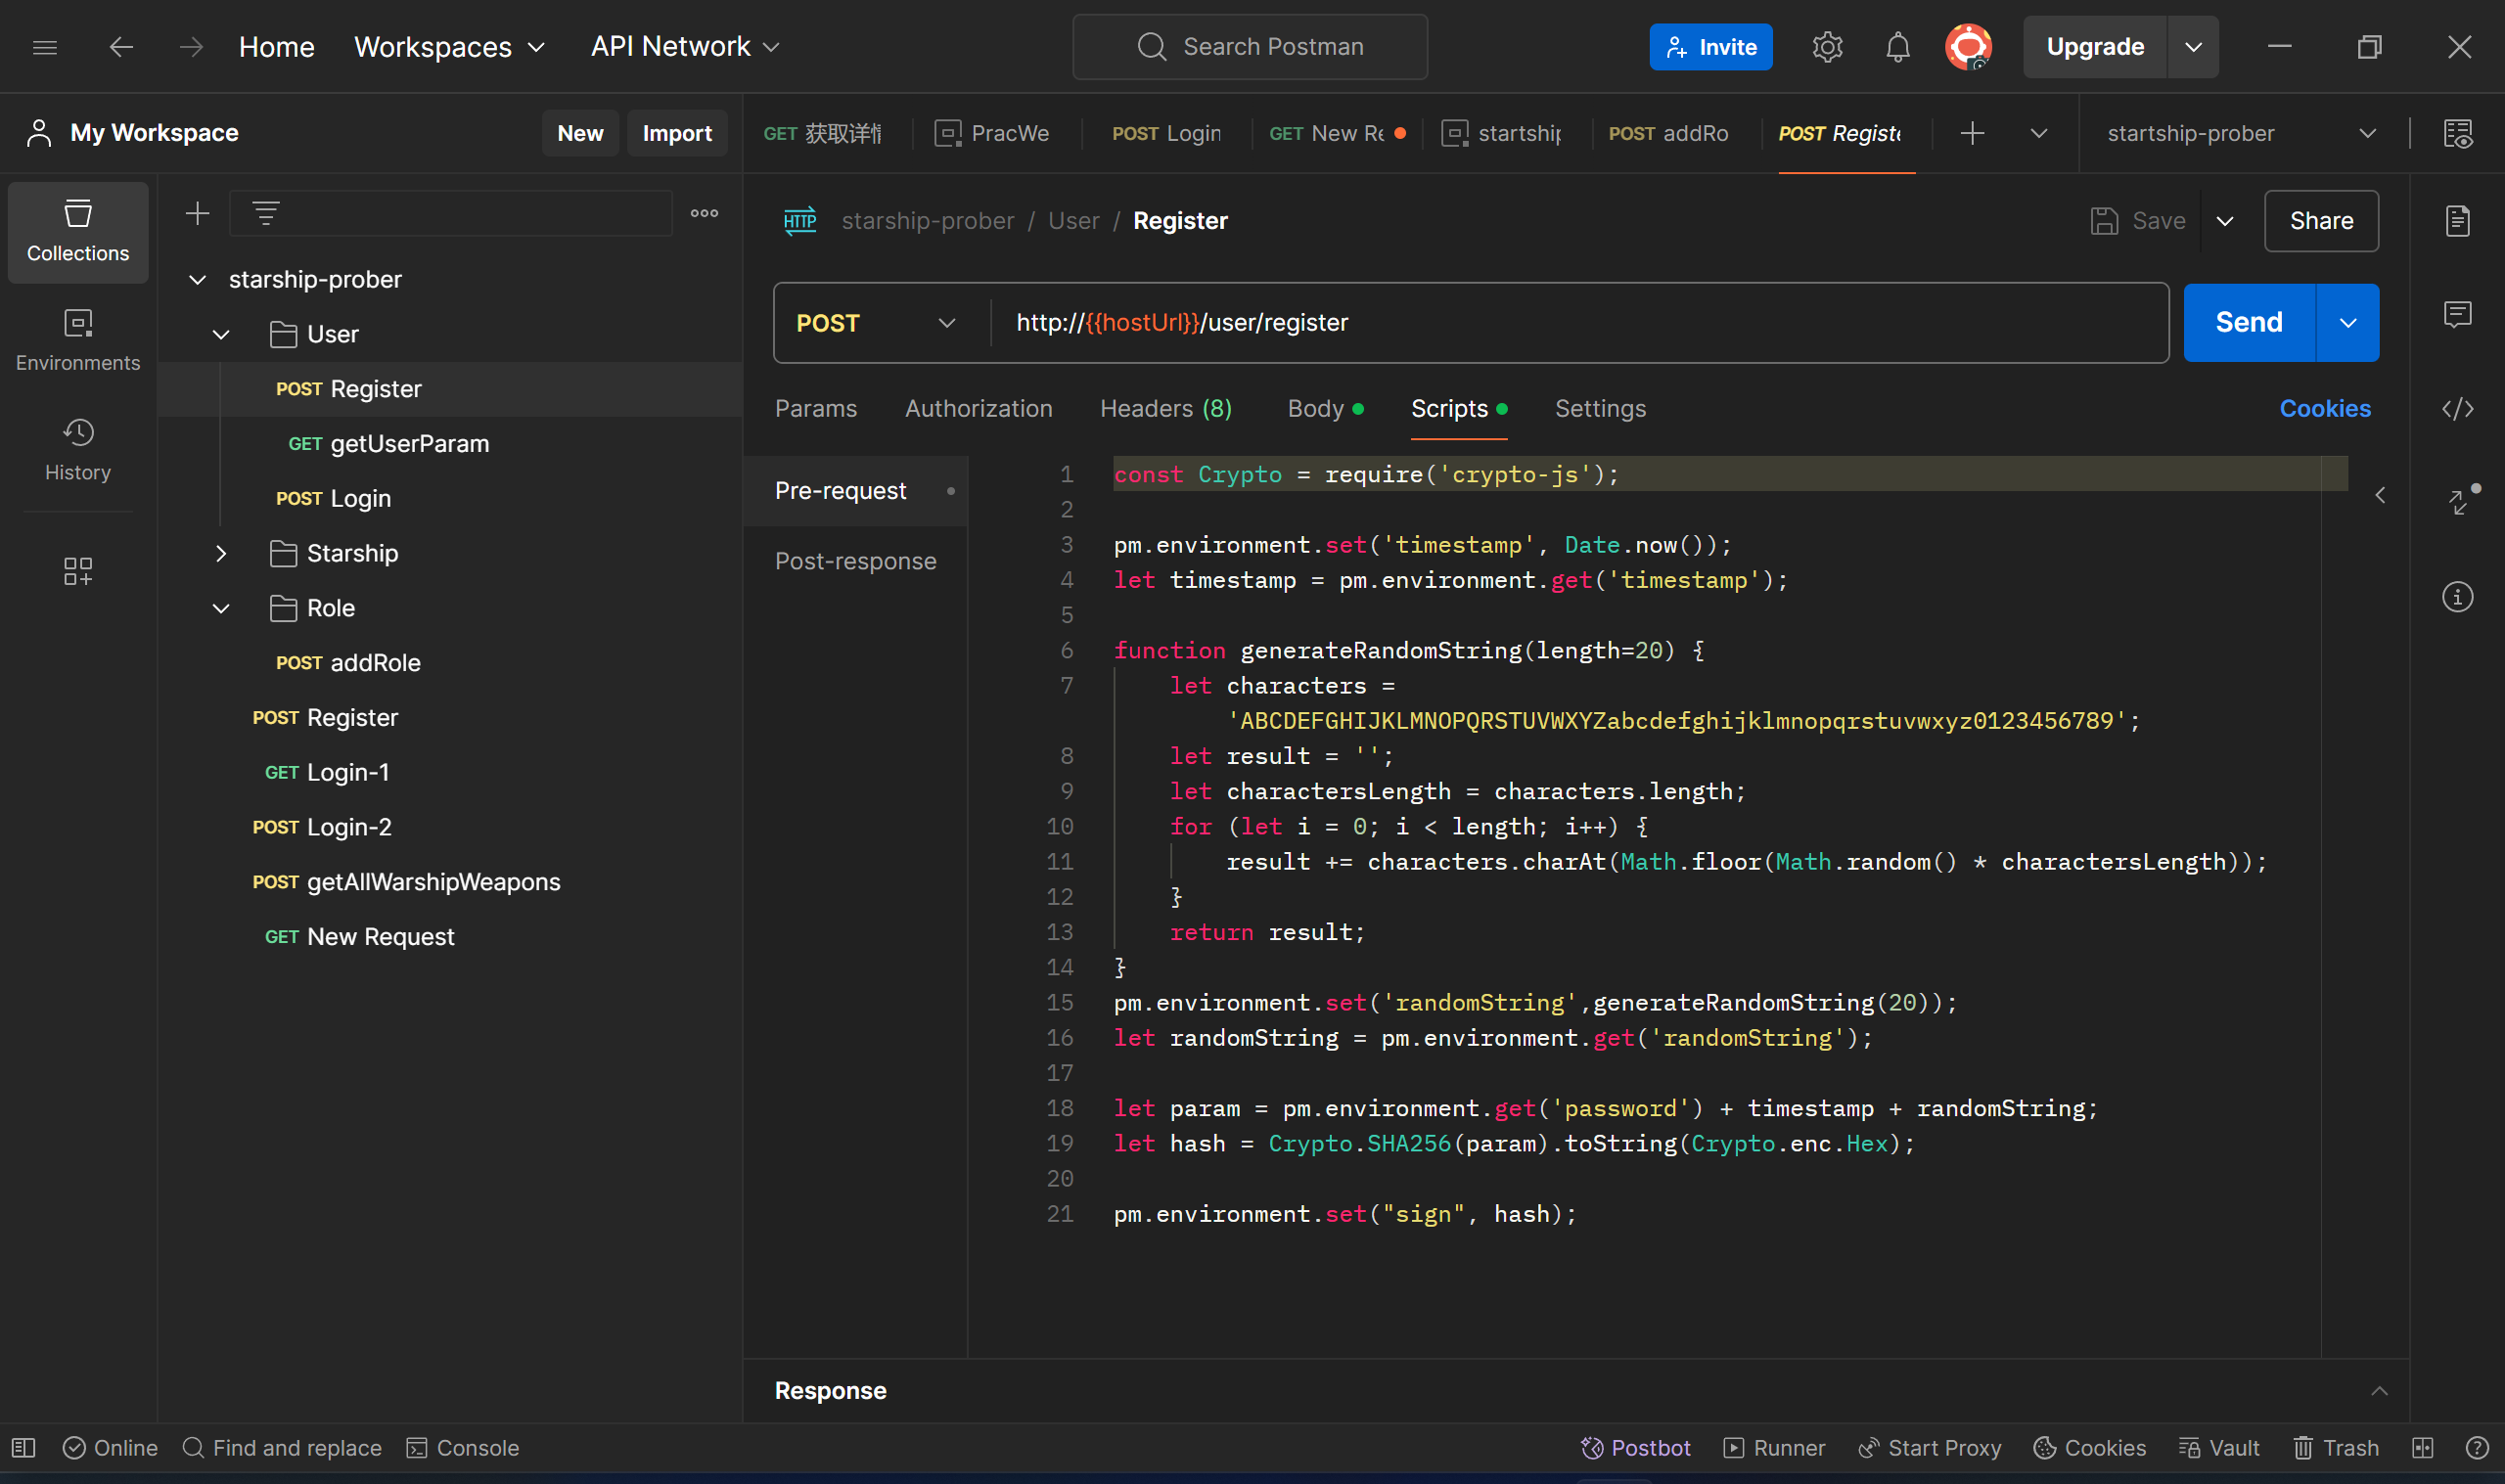
\includegraphics[width=\linewidth]{images/TestUserLogin}
	\caption{测试后端用户注册。编写了 Pre-request 脚本用于执行 SHA-256 算法。}
	\label{fig:testuserlogin}
\end{figure}

% TODO: \usepackage{graphicx} required
\begin{figure}[H]
	\centering
	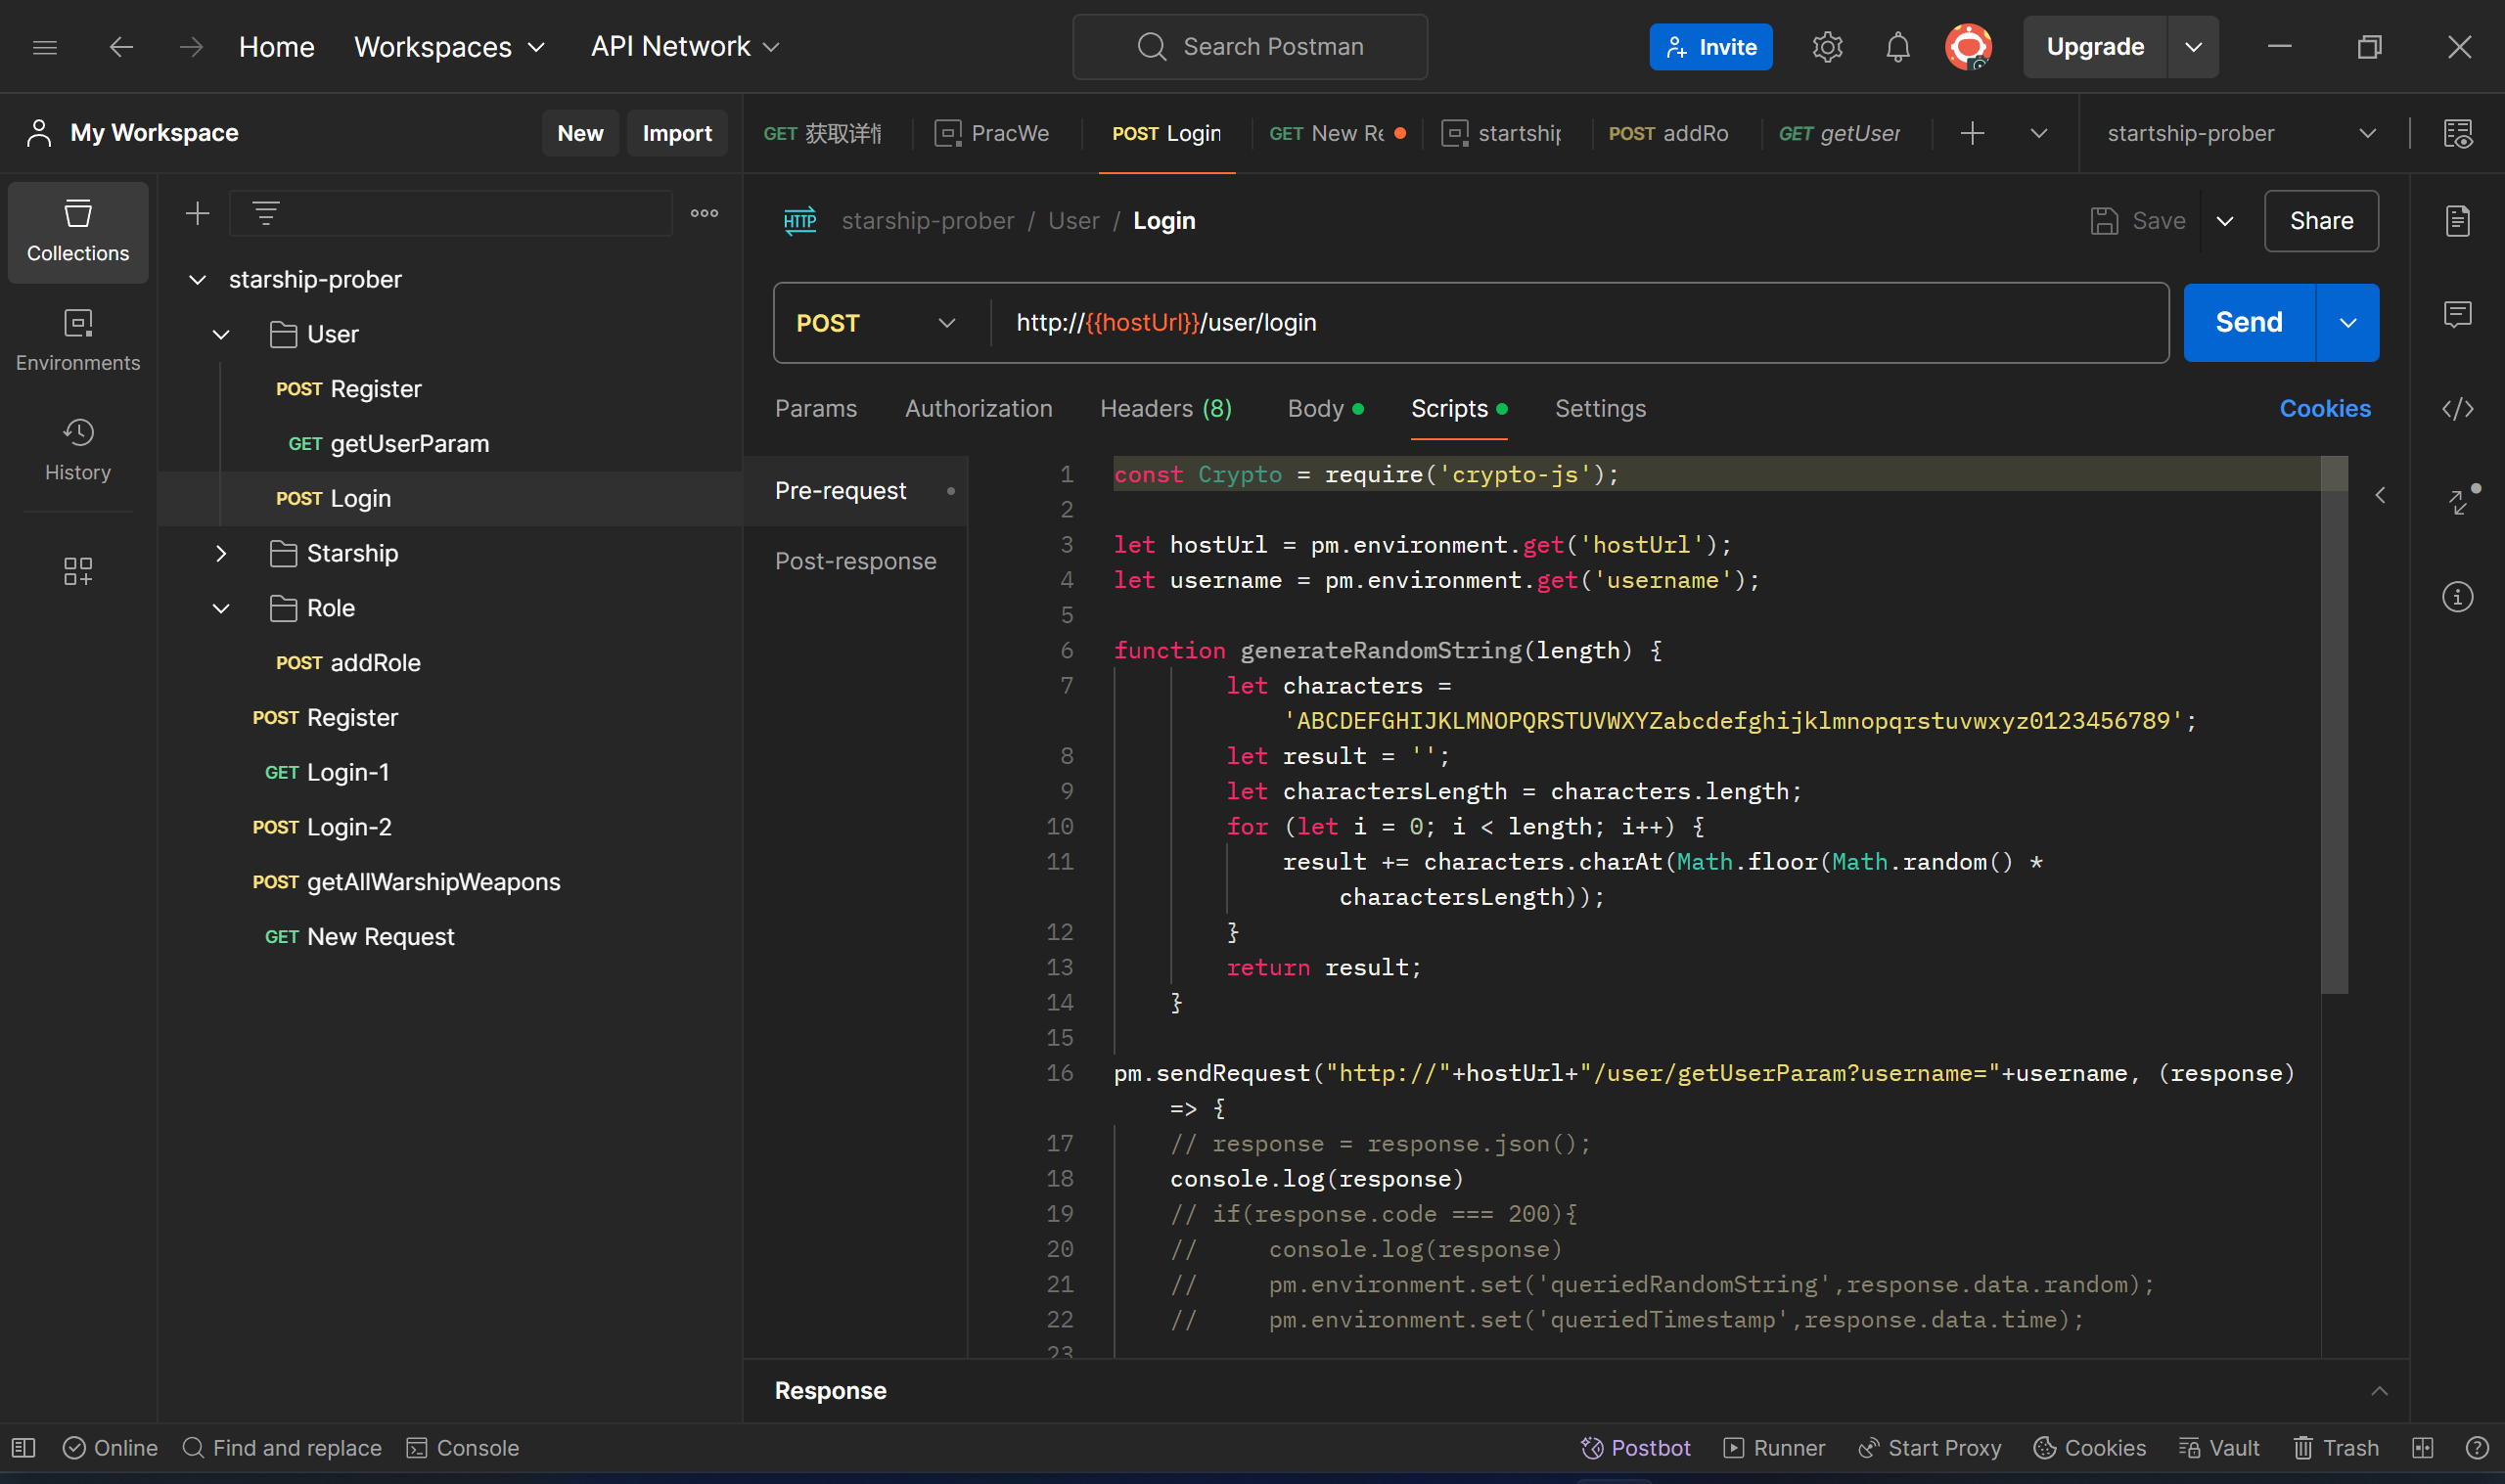
\includegraphics[width=\linewidth]{images/TestUserRegister}
	\caption{测试后端注册。同样编写了 Pre-requests。}
	\label{fig:testuserregister}
\end{figure}

% TODO: \usepackage{graphicx} required
\begin{figure}[H]
	\centering
	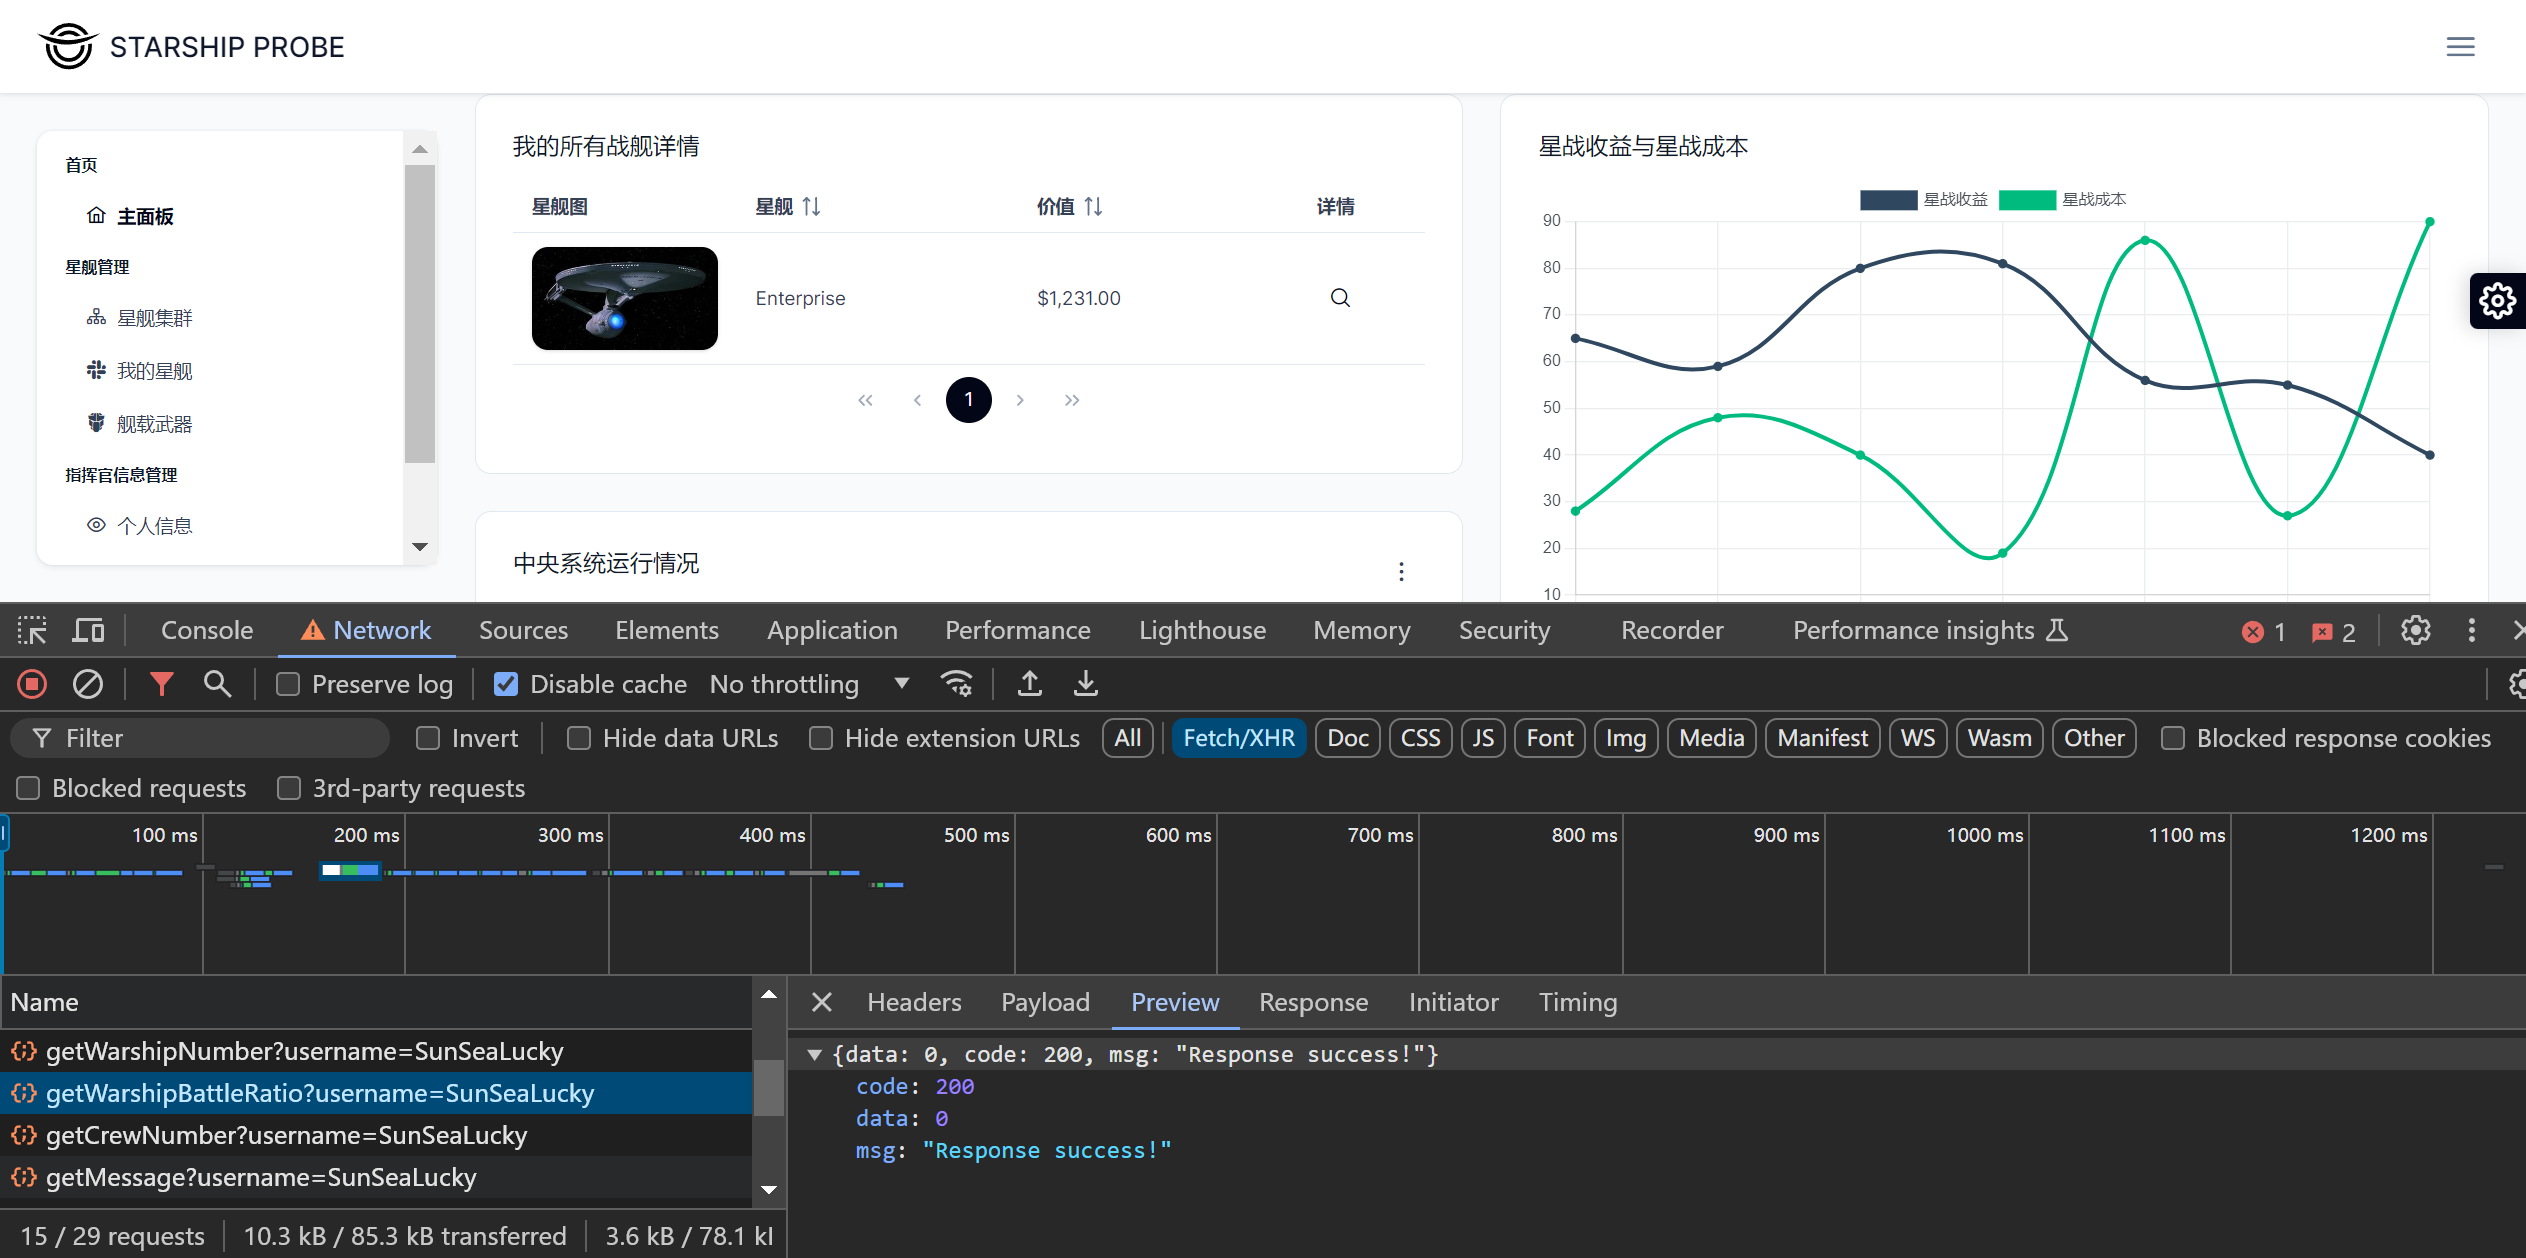
\includegraphics[width=\linewidth]{images/TestUserLoginFrontEnd}
	\caption{前端测试登录请求。熟练掌握 Network 和 Console,对前端开发效率提升会很大。}
	\label{fig:testuserloginfrontend}
\end{figure}

\section{存在的问题与总结}

\subsection{存在的问题}

系统采用 Spring Boot 和 Vue.js 技术栈,这两个框架虽然成熟,但集成过程中可能会遇到兼容性问题,如前端与后端的接口对接、数据格式不统一等。

通过问卷调查和访谈了解用户需求,但实际开发中可能会发现用户需求理解不够深入或需求变化频繁,导致系统功能反复修改,影响开发进度。

系统涉及用户登录、注册及个人信息管理,需要确保用户数据的安全和隐私保护。用户密码的加密存储、防止SQL注入和跨站脚本攻击等安全措施需要严格实施。

系统需要支持并发用户访问,至少支持100个用户同时在线。后端服务和数据库的性能优化是关键,否则可能影响用户体验。

系统应具有较高的稳定性,运行过程中无重大故障。数据备份和恢复机制需要设计到位,防止数据丢失。

系统代码需要具有良好的注释和文档,便于后续维护和升级。系统的模块化设计和代码结构需要考虑未来的功能扩展和修改。

前端页面设计需要简洁、美观,操作流程应简便。实际开发中可能会发现用户界面设计不够直观,或者用户操作流程不够流畅,需要不断优化。

系统测试包括单元测试、集成测试和用户测试,但实际开发中可能会发现测试用例覆盖不全面,导致一些功能缺陷或性能问题在上线后才被发现。

使用的数据库、前端框架和后端框架虽然流行,但可能存在技术过时或社区支持不足的风险,影响系统的长期维护和升级。

开发团队需要有效管理项目进度和协调各成员的工作,实际开发中可能会遇到任务分配不均、沟通不畅等问题,影响项目进度和质量。

\subsection{总结}

星舰管理系统的开发项目以经典电影《星际迷航》为主题,为《星际迷航》爱好者提供一个管理和查询星舰信息的平台。本项目采用 SpringBoot 和 Vue 技术栈,设计并实现了用户登录与注册、星舰管理、武器管理和用户信息管理等功能模块。

在开发过程中,通过文献综述法和问卷调查法,充分了解了《星际迷航》的背景和用户需求,为系统的设计和实现提供了理论支持和实践依据。尽管在技术集成、需求变更、数据安全和用户体验等方面存在一些挑战,但通过合理的设计和有效的管理,系统可以满足预期的功能和性能要求。

未来系统可以根据用户的反馈和需求不断进行功能扩展和性能优化,以提供更好的用户体验和更丰富的功能。开发团队需要继续关注技术的发展和用户需求的变化,保持系统的先进性和实用性。

通过本次项目的开发,我够在实践中提升开发技能,掌握 SpringBoot 和 Vue 等技术的应用,还能够在项目管理、团队协作和问题解决等方面得到锻炼,为未来的学习和工作打下坚实的基础。

\bibliographystyle{plain}
\bibliography{references}

\noindent[1] P. Domingos, “A few useful things to know about machine learning,” Commun. ACM, vol. 55, no. 10, pp. 78–87, Oct. 2012, doi: 10.1145/2347736.2347755.

\noindent[2] Q. Wang, “Analysis of the incidence and influencing factors of frailty among the elderly in Chinese communities,” Journal of Southern Medical University, vol. 41, no. 11, pp. 1719–1724, Nov. 2021, doi: 10.12122/j.issn.1673-4254.2021.11.18.

\noindent[3] S. V. Wilson, B. Cebere, J. Myatt, and S. Wilson, AnotherSamWilson/miceforest: Release for Zenodo DOI. (Dec. 12, 2022). Zenodo. doi: 10.5281/zenodo.7428632.

\noindent[4] S. Wen, “Calculation of Care Needs and Care Costs of Disabled Elderly in China - Based  on 2013 CHARLS National Baseline Survey”.

\noindent[5] “CHARLS database.” Accessed: Apr. 04, 2024. [Online]. Available: https://charls.charlsdata.com/pages/Data/2015-charls-wave4/zh-cn.html

\noindent[6] N. Shrestha, “Detecting Multicollinearity in Regression Analysis,” American Journal of Applied Mathematics and Statistics, vol. 8, no. 2, Art. no. 2, Jun. 2020, doi: 10.12691/ajams-8-2-1.

\noindent[7] He N., “Detection of cognitive impairment among the elderly in China and its relationship with sleep duration - an empirical analysis based on the 2018 CHARLS data,” Chinese Journal of Gerontology, doi: 10.3969/j.issn.1005-9202.2023.07.056.

\noindent[8] Z. Arvanitakis, R. C. Shah, and D. A. Bennett, “Diagnosis and Management of Dementia: Review,” JAMA, vol. 322, no. 16, pp. 1589–1599, Oct. 2019, doi: 10.1001/jama.2019.4782.

\noindent[9] J. Lee Ray, “Explaining Interstate Conflict and War: What Should Be Controlled for?,” Conflict Management and Peace Science, vol. 20, no. 2, pp. 1–31, Sep. 2003, doi: 10.1177/073889420302000201.

\noindent[10] X. Zhao et al., “Longitudinal Relationship Between Frailty and Cognitive Impairment in Chinese Older Adults: A Prospective Study,” J Appl Gerontol, vol. 41, no. 12, pp. 2490–2498, Dec. 2022, doi: 10.1177/07334648221118352.

\noindent[11] R. Guo, “Master ’s thesis on prediction of preeclampsia based on SAM-Voting,” 2022, doi: 10.27009/d.cnki.gdblu.2022.001069.

\noindent[12] F. E. Harrell, Regression Modeling Strategies: With Applications to Linear Models, Logistic and Ordinal Regression, and Survival Analysis. in Springer Series in Statistics. Cham: Springer International Publishing, 2015. doi: 10.1007/978-3-319-19425-7.

\noindent[13] X. Zhou, “Research on the demand forecast of China ’s elderly care workers based on Markov model”.

\noindent[14] Wang  tao and Guo Z., “Research progress in diagnosis and treatment of mild cognitive impairment,” Western Medicine, vol. 31, no. 9, 2019.

\end{document}